\documentclass{gatech-thesis}
% The default options:
%   \documentclass[11pt,letterpaper,oneside,%
%       doublespaced,normalmargins,final]{gatech-thesis}
% will generate a document that conforms to the graduate studies office
% guidelines.
 \ifx\pdfoutput\undefined
   \usepackage[dvips,final]{graphicx}  % using latex+dvips
   \usepackage[dvips,usenames]{color}
   \else
   \usepackage[pdftex,final]{graphicx} % using pdflatex
   \usepackage[pdftex,usenames]{color}
 \fi
 \usepackage{epstopdf}
 \usepackage{amssymb}
\usepackage{amsmath}
\usepackage{amsbsy}
\usepackage{wrapfig}
\usepackage{changebar}
\usepackage{xcolor}
\usepackage{rotating}
\usepackage[ruled,linesnumbered,vlined]{algorithm2e}
\usepackage[normalem]{ulem}
\DeclareMathOperator{\sgn}{sgn}
\input{defs}
%define stuff in preamble
 \degree{Doctor of Philosophy}
 \department{College of Computing}
 \title{Locomotion Synthesis in Complex Physically Simulated Environments}
 \author{Jie Tan}
 \principaladvisor{Karen Liu}
 \principaladvisors{Greg Turk}
% \committeechair{Greg Turk}
 \firstreader{Jarek Rossignac}
 \secondreader{Frank Dellaert}
 \thirdreader{James O'Brien}[Department of Electrical Engineering and Computer Science][University of California at Berkeley]
 \submitdate{December 2015}
 \approveddate{October 23, 2015}
 \copyrightyear{2015} %add one if thesis submitted in Dec.

% \thesisproposalfalse       % default
% \titlepagetrue             % default
% \signaturepagetrue         % default
 \copyrighttrue            % default
% \figurespagetrue           % default
% \tablespagetrue            % default
% \contentspagetrue          % default
% \dedicationheadingfalse    % default
% \bibpagetrue               % default
% \strictmarginstrue         % default

\bibfiles{avc-bib}

\begin{document}
\bibliographystyle{gatech-thesis}
\setchaptertocdepth{2}
%
\begin{preliminary}
\begin{acknowledgements}
First, I want to thank my advisors, Greg Turk and Karen Liu. It is a great pleasure to work with you two in the last six years. You serve as great role models not only in research but also in life. I feel that I am deeply indebted to both of you. You have built up a huge portion of knowledge that I possessed today. You encouraged me to pursue my interests and to follow my passion. You taught me how to think creatively and helped me develop rigorous procedures to approach research problems. More importantly, you helped me build my confidence, especially in my first years in US when I was facing language and culture barriers. I feel extremely fortunate to have you as my advisors. Without your guidance, I would be nowhere as successful as I am today. I believe that what I have learned from you in the last six years will carry on to influence me and benefit me throughout my whole life.

I want to thank the members of my thesis committee: Jarek Rossignac, Frank Dellaert and James O'Brien as well as my qualifier committee members: Irfan Essa and Blair Macintyre. Each of you has helped me become a stronger researcher in your own way. You have broaden my knowledge, shaped my rigorous thinking, taught me effective ways of communication and helped me develop social skills.

I also want to thank my friends and labmates: Huamin Wang, Chris Wojtan, Sumit Jain, Yuting Ye, Karthik Raveendran, Mark Luffel, Tina Zhuo, Yunfei Bai, Sehoon Ha, Kristin Siu, Albert Li, Yangfeng Ji, Alexander Zook, Alex Clegg, Edward Liu, and many more. Thank you for your helpful discussions with me about my research, my presentation and my life.

Finally, I want to thank my family. I want to thank my wife, Yuting, for your unlimited support every day throughout my PhD journey. I also want to thank you for your understanding, especially for your help on modeling, rendering and video editing before each SIGGRAPH deadline. I want to thank my parents, Yangsun and Xiuchun. It is you that shaped me into who I am today. I am extremely grateful to your guidance and supports.

\end{acknowledgements}
%
\contents
%
\begin{summary}
Understanding and synthesizing locomotion of humans and animals will have far-reaching impacts in computer animation, robotic and biomechanics. However, due to the complexity of the neuromuscular control and physical interactions with the environment, computationally modeling these seemingly effortless locomotion imposes a grand challenge for scientists, engineers and artists. The focus of this thesis is to present a set of computational tools, which can simulate the physical environment and optimize the control strategy, to automatically synthesize locomotion for humans and animals.

We first present computational tools to study swimming motions for a wide variety of aquatic animals. This method first builds a simulation of two-way interaction between fluid and an articulated rigid body system. It then searches for the most energy efficient way to swim for a given body shape in the simulated hydrodynamic environment.

Next, we present an algorithm that can synthesize locomotion of soft body animals that do not have skeleton support. We combine a finite element simulation with a muscle model that is inspired by muscular hydrostat in nature. We then formulate a quadratic program with complementarity condition (QPCC) to optimize the muscle contraction and contact forces that can lead to meaningful locomotion. We develop an efficient QPCC solver that solves a challenging optimization problem at the presence of discontinous contact events.

We also present algorithms to model human locomotion with a passive mechanical device: riding a bicycle in this case. We apply a powerful reinforcement learning algorithm, which can search for both the parametrization and the parameters of a control policy, to enable a virtual human character to perform bicycle stunts in a physically simulated environment.

\del{Finally, we explore the possibility to transfer the controllers designed in a simulation to the real humanoid robots. We tackle the challenge of \emph{Reality Gap} by calibrating the physical simulation to match the data measured in the real-world experiments.}
\newtext{Finally, we explore the possibility to use the computational tools that are developed for computer animation to control a real robot. We develop a simulation calibration technique which reduces the discrepancy between the simulated results and the performance of the robot in the real environments. For certain motion planning tasks, this method can transfer the controllers optimized for a virtual character in a simulation to a robot that operates in a real environment.}

\end{summary}
\end{preliminary}
%
\chapter{Introduction}

Most of us human can effortlessly accomplish various locomotion tasks. We can walk, run, jump and even ride on a bicycle. In addition, Mother Nature has created an amazingly diverse set of motions in the animal kingdom. For example, birds can fly in the sky, fishes can swim in the water, geccos can crawl on a verticle surface and cats can reoriented themselves to survive a fall. Understanding and synthesizing these motions will have far-reaching impacts on a wide variety of industries, including entertainment, robotics and health care. In the entertainment industry, such as movie and games, we need to study the locomotion in nature to faithfully reproduce them on the screen, or to synthesize plausible animations for imaginary creatures. Studying  locomotion in nature can help us develop robotic controllers with extensive agility and maneuverability, such as MIT Cheetah \cite{} and Big Dog from Boston Dynamics \cite{}. These robots are expected to accomplish various missions, which are dangerous for human operators, in military, transportation, exploration and rescuing. Understanding human locomotion, can guide us build comfortable and yet powerful exoskeletons that can promote gait habilitation in children, assist paralyzed person to walk or aid normal persons to achieve superhuman ability.

Although we often take our locomotion ability for granted because we can perform them so effortlessly, it is a notoriously difficult problem because locomotion involves sophisticated neuromuscular control, sensory information processing, motion planning, coordinated muscle activation, and complicated interactions between the body and its physical environment. Despite extensive study for centuries, we have not yet fully understood the underlying physics and control mechanisms of these motions. It poses a grand challenge for scientists, engineers and artists. The focus of this thesis is to present a set of powerful computational tools that facilitate the study of the locomotion of humans and animals, for the applications in computer graphics and robotics.

\section{State of the Art}

In computer graphics, the most popular techniques to synthesize motions are key frames or motion capture. Although both methods have produced realistic character animations and special effects in movies (Toy Story \cite and Avatar \cite{}), they are not scalable and generalizable ways to synthesize motions. The key-frame method requires artistic expertise and laborious manual tuning. As a result, generating animations is a time-consuming and tedious task. For example, an 100-minute animated feature film produced by Pixar typically takes more than five years of development. On the other hand, the motion capture not only requires expensive equipment and tedious postprocessing, it is difficult to reuse the recorded data in other situations. A more principled way to synthesize motions of humans and animals is to computationally mimic the natural process that have shaped our motions. Our motions are shaped through millions of year of evolution in a world that obey physical laws. The paradigm of physically-based character animation first builds physical simulation and then optimize the motions of the character in the physically-simulated environment. Using this paradigm, many natural motions, including walking \cite{}, running \cite{}, flying \cite{} and swimming \cite{} emerge automatically from the optimization solution. In addition to these basic locomotion tasks, the research in this field has developed algorithms that allow virtual characters to recover balance from unexpected perturbations, to move in different styles, to navigate through rough terrains and to demonstrate highly skillful stunts.

Similarly, we have also seen impressive robotic systems developed in the last decade. The MIT Cheetah can run up to 20 miles per hour and jump over obstacles. Other quadrupedal robots from Boston Dynamics, Big Dog and Little Dog, can walk robustly in adversary environments, including icy or rocky terrains. The soft body robots can take advantage of their flexible bodies to navigate narrow and unstructured spaces. The humanoid robots, such as Petman and Asimo, are able demonstrate a repertoire of locomotion skills, including walking, running, dancing and climbing stairs. These amazing advance in robotics are largely attributed to the use of computational tools, including simulation, optimal control and reinforcement learning. Although these coputational tools are becoming popular and have automated some portions of the development process, the task of locomotion controller design are still limited to experts and relies on tedius manual tuning.

Despite the impressive achievements in computer graphics and robotics, the gracious, agile and diverse motions of the real creatures are far from being reproduced. Synthesizing realistic motions turns out to be a challenging problem. First of all, we are facing tremendous challenges in faithfully simulate the physical environment. For example, we have not found accurate mathematical models to describe certain physical phenomena while some dynamical systems are computationally expensive or even infeasible to simulate. More importantly, locomotion tasks often involve forceful interactions between two dynamical systems, the character itself and the surrounding environment. Since these two systems are often governed by different types of equations and simulated with different algorithms, modeling the two-way interaction between them presents a nontrivial task. An accurate and efficient physical simulator is not enough. Without proper control of muscle contactions and joint torques, a virtual character cannot move in a meaningful way to achieve an intended goal. Finding a good control mechanism poses a different set of challenges. One of the challenges is under-actuation. The movement of the center of mass (COM) can only be achieved indirectly through carefully planned interactions, such as contact, with the environment. Balance is another big challenge in locomotion. Humans and many animals are inherently unstable because their COM are above the supporting feet. The characters that we wish to control may have a large number of muscles (actuators), which need to be activated in a coordinated fashion. This results in a high dimensional nonconvex optimization problem, which can be computationally infeasible. Motion optimizing with physical constraints introduces additional difficulties. For example, the state-of-the-art contact models can invalidate the gradient, which is essential in modern optimization solvers.

Generally speaking, controlling high-dimensional dynamic systems, governed by highly nonlinear differential equations and coupled through complex mechanisms, is considered a nearly unsolvable problem. As a result, most of the prior research make simplifications on simulation models and optimization algorithms to make the computation tractable. However, many of these simplifications were made without considering the optimality of the control problems. In this thesis, we will investigate some of these simplifications and develop novel algorithms for those components that should not be simplified. 


\section{Thesis Overview}

This thesis presents a set of computational tools to study locomotion in complex physical environments. Two common algorithmic components across all the works in this thesis are physical simulation and motion optimization. In contrast to prior works that use simplified physical models, we develop new algorithms to improve and to combine the state-of-the-art simulation and optimization techniques to tackle the challenges of motion synthesis. We start with a survey of related work in the fields of computer graphics and robotics (Chapter 2). We then investigate motor control for various locomotion tasks in a hydrodynamic environment (Chapter 3), for soft body characters (Chapter 4) and with a passive mechanical device (Chapter 5). In Chapter 6, we explore the techniques to transfer the controllers developed in the simulation to robots operating in the real world. We conclude the thesis with conclusions and suggestions for future work (Chapter 7).

\subsection{Locomotion in Hydrodynamic Environment}



\begin{figure}[!h]
  \centering
    \includegraphics[width=\textwidth]{figures/teaserSwimming.eps}
  \caption{Aquatic creatures swim in a physically simulated hydrodynamic environment.}
  \label{fig:teaser1}
\end{figure}

The oceans covers over seventy percent of the area on our planet. They contain a wide variety of creatures that use swimming as their primary form of locomotion. Scientific studies show that the swimming gaits of the aquatic creatures are highly efficient compared to the man-made underwater vehicles. Studying their swimming motions could help us discover better propulsion mechanisms and design more efficient undersea vehicles to explore the largest uncharted territory on our planet. In Chapter 3, we apply numerical optimization to automatically discover the most energy efficient swimming gaits for given aquatic creatures in a physically-simulated hydrodynamic environment.

A main challenge in physical simulation is to model the complex interaction between two different types of dynamic systems, such as the two-way coupling between the fluid and a swimmer represented as an articulated rigid body system. We present an accurate physical simulator \cite{} that simultaneously solves the Navier-Stokes equations for fluids, the Lagrangian dynamics for an articulated rigid body and matches their accelerations at fluid-solid boundaries. The simulation results of swimming fish and eels show vortex trails that are in agreement with laboratory measurements.

Simulating fluid itself is hard; optimizing locomotion in a hydrodynamic environment is even more challenging. Previous methods have resorted to simplified fluid models. However, studies have shown that fish takes advantage of surrounding vortices, which are omitted in the simplified models, to provide energy boosts. Incorporating an accurate Navier-Stokes fluid model in the simulation presents new challenges in controller optimization: The optimization space is full of local minima due to the chaotic fluid behavior. Evaluating the gradient of the objective function is time-consuming. We demonstrated that sampling-based optimization algorithms, which are robust to local minima and are gradient free, are effective tools to overcome these challenges. This approach found efficient swimming motions that are comparable to those of real-world animals (Figure \ref{fig:teaser1}). 

\subsection{Locomotion for Soft Body Characters}

\begin{figure}[!h]
  \centering
    \includegraphics[width=\textwidth]{figures/teaserSoftBody.eps}
  \caption{Four alphabetic soft body characters perform different forms of locomotion.}
  \label{fig:teaser2}
\end{figure}

While most research in character animation and robotics focus on characters that are made exclusively from rigid parts, we have seen an increasingly amount of efforts in the last few years to develop soft body robots \cite{}. While these research demonstrates a huge potential of soft body robots and their broad applications, it demands a new set of computational tools to study and to synthesize motions for soft body characters.

To model soft body characters, we not only need to simulate the passive dynamics of deformation, but also the actuation of muscles. In Chapter 4, we present a new mathematical model for artificial muscles that are motivated by the muscle structures of soft body animals in nature. Similar to real muscles, these artificial ones are arranged in groups and only allowed to contract. Complex movements need to be accomplished by the coordinated contraction of multiple muscle groups. We develope a finite element method with this muscle model to simulate soft body animals.

Optimizing controllers in the presence of discontinuous contact forces is a long-standing problem. Controlling locomotion for soft body characters (Figure \ref{fig:teaser2}) exacerbates the difficulty. The deformation of the body constantly changes the contact configuration between the character and the ground. A common practice is to separate contact planning and controller optimization. We identify that this simplification eliminates effective control strategies, and this causes the soft body character to lose balance. We derive an elegant solution to this problem that combines contact planning with controller optimization. We formulate a quadratic program with complementarity conditions (QPCC) and worked out an efficient solver for QPCC derived from control problems with contacts. As a result, effective control strategies emerge automatically from the QPCC solution.

\subsection{Locomotion with Mechanical Devices}

\begin{figure}[!h]
  \centering
    \includegraphics[width=\textwidth]{figures/teaserBicycle.eps}
  \caption{A human character performs stunts on a road bike, a BMX bike and a unicycle.}
  \label{fig:teaser3}
\end{figure}

Human has invented numerous mechanical tools to ease our life. Robots in the future can work much more efficiently if they can take advantage of these existing tools. Instead of manually program the robots to master each tool, we hope that they can learn how to use them autonomously. Learning to ride a bicycle is an excellent case study. The bicycle, which has greatly boosted the efficiency of locomotion, was voted as the best invention since the 19th century. Even though the dynamics of bicycles is relatively well-understood, riding a bicycle is challenging due to the inherently unstable dynamics. Controlling balance on a bicycle involves sophisticated and robust neuromechanical control, which is vital for many locomotin tasks. In Chapter 5, we present a machine learning algorithm that allows a virtual character to learn to ride a bicycle in a physically simulated environment. 

In addition to the basic maneuvers, we hope that the character can learn more challenging but visually spectacular stunts (Figure \ref{fig:teaser3}). Performing stunts requires fast reaction, precise control and years of practice, and this challenges the best human riders. When we optimize the control policies for bicycle stunts, we find that the widely-used assumption of a predetermined controller parameterization severely limits the search space and leaves the hard work to the user to design a good parameterization. We decide that optimizing the parameterization automatically is equally important as optimizing the parameters. Our algorithm evolves both the policy parameterization and the parameters simultaneously. This significantly improves the quality of the resulting controllers. Eventually, our simulated characters learn to perform a wide variety of bicycle stunts within hours, which is even faster than the best human stunt bikers.

\subsection{Locomotion Controller Transfer from Virtual to Real World}

Above three works demonstrate that with the powerful computational tools for character animation, natural, agile and robust motions can be synthesized efficiently and autonomously. However, creating lifelike robots is still an extremely challenging, trial-and-error process that is restricted to experts. The fast evolution of 3D printing technology will soon trigger a shift in the robotics industry from mass production to personalized design and fabrication, which will result in an immediate need for a faster, cheaper and more intuitive way to design robotic controllers. The computational tools we developed can potentially automate and streamline the process if we can transfer the controllers from the virtual simulation to the real world.

Transfering controllers optimized in a simulation onto a real robot is a non-trivial task. A controller that is optimized even using a state-of-art simulation often does not work in a real environment. This is known as the \emph{Reality Gap} \cite{}. This gap is caused by various simplifications in the simulation, including inaccurate physical model, unmodeled actuator dynamics, assumptions of perfect sensing and zero latency. In Chapter 6, we investigate some of these simplifications and present a general framework of simulation calibration. Simulation calibration optimizes simulation parameters to minimize the discrepancy between the data collected from real experiments on the robot and that generated in the simulation. After calibration, the simulation becomes more faithful to the real-world dynamics. Controllers that are designed with the improved simulator can work in both the virtual and the real world. 

\section{Contributions}

The computational tools presented in this dissertation provide several contributions to the communities of character animation and robotics. These contributions are as follows.

\paragraph{A stable simulation of two-way coupling between fluids and articulated rigid bodies.} We present a novel swimming simulator that can simultaneously solve the dynamics of fluids, articulated rigid bodies and their two-way interactions. Compared to the traditional two-way coupling solver that alternates the fluid update and the the rigid body update, our method is more numerically stable. We are able to use time steps of 33ms for all our experiments without any stability problem. Using larger time steps makes our simulation orders of magnitudes faster than the alternating solver. As a result, we can discover a swimming pattern with up to days of computation while using the traditional two-way coupling technique can take weeks.

\paragraph{A finite element simulation with a muscle model for soft body animals.} Based on the muscle structure of muscular hydrostat \cite{} in real soft body animals, we develop a muscle model for the simulated characters. Combined with the finite element method for the passive deformation of the body, it provides intuitive ways to control the character in a coordinated manner. The use of this muscle model not only reduces the dimensionality of the control problem and but also results in natural-looking motions.

\paragraph{A optimizatoin solver for quadratic program with complimentarity conditions.} Controlling locomotion with contacts is a long-standing problem in continuous optimization because change of contact situation (static, sliding or breaking) can introduce discontinuities to the dynamics. A commonly-used technique is to mannualy specify the contact situation and only optimize the forces under the prescripted contact situations. However, this could eliminate effective locomotion strategies. We solve this problem by formulating a generic quadratic program with complimentarity conditions. We also develop an efficient solver for QPCC problems with contacts. This method can optimize both the contact situation and forces simultaneously. As a result, many interesting and effective locomotion strategies emerge automatically from the QPCC solution.

\paragraph{A reinforcement learning algorithm that searches both the parametrization and the parameters of a policy.} We present the first reinforcement learning algorithm which demonstrate that extremely challenging locomotion tasks, such as bicycle stunts, can be learned efficiently in simulation. Most of the stunt actions are learned within one hour, which is even faster than the best human stunt biker. These results present a new benchmark for future research in reinforcement learning. The key to such an efficient learning algorithm is an evolutionary optimization that can search for the parametrization and the parameters of a control policy simultaneously. We believe that this reinforcement learning algorithm can be generalized to master other challenging locomotion tasks.


\chapter{Related Work}

This chapter presents a summary of previous work that is most relevant to our methods. The two key components of our computational tools are physical simulation and controller optimization. We will begin with a brief review of related work in these two fields. Since the ultimate goal of our research is an end-to-end computational framework that can autonomously design robotic controllers from high-level task specifications, we need to transfer the controllers found in the simulation to the real robots. We will conclude this chapter with an overview of related works in controller transfer from virtual to real environments in robotics.

\section{Physical Simulation}
In order to simulate the physical environment, researchers often borrow numerical tools from the applied mathematics literature. The most widely used methods include Eulerian methods \cite{Foster:1996,stam99stablefluids}, Lagrangian methods \cite{Premzoe03,Muller:2003}, Hybrid methods \cite{Fan:2013} and position-based dynamics \cite{Muller:2007,Macklin:2014}. These methods have produced realistic simulations for a wide variety of dynamical systems, such as rigid bodies, deformable bodies, fluids and clothes. In the next few sections, we will focus on simulation of fluids, soft bodies, contacts and bicycle dynamics, which are used in our work.

\subsection{Fluids}

Simulating fluids involves numerically solving the governing equations of motions, Navier-Stokes equations. Two popular methods in computer animation are Lagrangian method and Eulerian method. The Lagrangian approach treats the fluid as a particle system \cite{Monaghan:1992,Premzoe03,Muller:2003,Raveendran:2011}. In contrast, the Eulerian approach treats the fluid as a continuous velocity field discretized
on a computational grid. Foster and Metaxas's work \cite{Foster:1996} was the first that
solved the full 3D Navier-Stokes equations to animate fluids.
Stam \cite{stam99stablefluids} improved it, achieving unconditionally
numerical stability by introducing the semi-Lagrangian
method for the convection term and implicit solver for
the viscosity and pressure terms. Although the Eulerian method is more computationally expensive, it has produced stunning visual results when simulating a wide range of physical phenomena, including fire and smoke\cite{Nguyen:2002,Fedkiw:2001}, explosion \cite{Yngve:2000}, surface tension \cite{Hong:2005,Wang:2005}, non-Newtonian fluid \cite{Goktekin:2004,Bargteil:2007} and multi-phase flow \cite{Losasso:2006,Ando:2015}. We choose to use the Eulerian method in Chapter 3 because it is easier to enforce the incompressibility condition of fluids, which turns out to be important in swimming motions. 

When studying swimming motions, simulating fluids alone is not enough. Swimming involves two-way interactions between the character and the fluid. Accurately modeling this two-way interaction is essential to simulate swimming motions. Many researchers have proposed various ways to
simulate the two-way coupling between fluids and solids.  Takahashi et al. \cite{takahashi2002fluid-rigid}
presented a simple alternating two-way coupling method. The velocities of the solid
objects served as the boundary conditions for the fluid motion while the
pressure field solved from the Navier-Stokes equations was integrated at the
solid surface to provide a net force and a net torque exerted on the solid
objects. Arash et al. \cite{arash2003simulatingfluid-solid} represented the solids by mass-spring models and fluids by marker particles.  The interactions were calculated through the mutual forces between the marker particles and mass nodes at the interface. Carlson et al. \cite{carlson2004rigid} proposed the rigid
fluid method that treated solids as fluids at first
and then projected the velocity field in the solid region onto a subspace
satisfying the rigid constraints. Guendelman et al. \cite{guendelman2005thin} made use of an
alternating approach that was generalized to include octree and thin
shells.  They solved the pressure field for a
second time by adding solid masses to the fluid grid density, which improves
the pressure field. Klingner et al. \cite{klingner2006mesh} used a tetrahedral mesh for accurate boundary discretization and extended the mass conservation (projection) step
to include the dynamics of rigid body. This was extended to model the interaction between fluids and deformable bodies \cite{chentanez2006simultaneous}. Batty et al. \cite{batty2007fast} derived a fast variationl approach that allowed sub-grid accuray using regular grids. Robinson et al. \cite{robinson2008two} developed a generic and momentum
conserving technique to couple fluids to rigid/deformable solids and thin
shells. The coupled system is symmetric indefinite and solved using MINRES. Our two-way coupling technique resembles that of Klingner et al. \cite{klingner2006mesh}. The main difference is that we simulate the interaction between fluids and articulated rigid bodies instead of rigid bodies. Furthermore, our represent of the articulated rigid body in the generalized coordinates further complicates the swimming simulation.

\subsection{Soft Bodies}
In Chapter 4, we study the locomotion on land for soft body characters. To simulate the squishy characters, we need a physical model for deformable objects.
Since the seminal work introduced by Terzpoulos
\cite{Terzopoulos:1987}, researchers in computer graphics have
simulated a wide variety of deformable phenomena including cloth
\cite{Baraff:1998,Bridson:2002}, elasticity \cite{Muller:2002}, and
plasticity \cite{O'Brien:1999,Bargteil:2007}. Although mass-spring systems \cite{Provot:1996,Liu:2013} are
widely-used due to its simplicity, it is difficult to
specify the spring stiffness to capture the desired material property. A more accurate technique is
the Finite Element Method (FEM) \cite{Bathe:2007}, which typically uses a
tetrahedral mesh to find weak solutions of the dynamic
equations. The robustness of FEM simulation can be improved by
handling inverted tetrahedra \cite{Irving:2004}, remeshing
ill-conditioned elements \cite{Bargteil:2007}, or preserving volume
without locking artifacts \cite{Irving:2007}. To improve the
performance of FEM simulation, linear strain model and precomputed
stiff matrix are often used. However, these models are only valid for
small deformations. To simulate large deformations, M\"{u}ller \etal
\cite{Muller:2002} proposed a corotational method to fix the
volume inflation artifacts. Nesme \etal \cite{NPF05} suggested
that linearization around the current deformed configuration reduces
ghost torques. Precomputed deformation modes have also been used to
interactively deform large structures
\cite{James:2003,Barbic:2005,Kim:2009}. In our work, we choose to use the corotational linear FEM \cite{Muller:2002,NPF05}
to simulate the soft body dynamics. We also use implicit integration to further increase the simulation stability and speed.

\subsection{Contact Modeling}
Locomotion on land is achieved by a character actively and purposefully pushing the ground. As a result, an equal and opposite ground reaction force is exerted on the character through the contacts and changes its center of mass. Modelling contacts between two dynamic systems is an active research area in physical simulation. Early simulations use penalty forces \cite{Terzopoulos:1987}, whose magnitude is proportional to the depth of penetration. Despite its simplicity, this method requires stringent simulation time steps and careful parameter tunning. More recently, constraint-based methods, such as linear complementarity problem (LCP), are used to handle contacts. Stewart and Trinkle proposed an
LCP formulation using an implicit time-stepping method to guarantee
non-penetration, directional friction, and approximated Coulomb's
friction cone conditions \cite{Stewart:1996}. Based on the LCP
framework, many improved contact models were introduced recently in
computer graphics, including using an efficient iterative method
\cite{Erleben:2007}, a simple staggered sequence of projections
\cite{Kaufman:2008}, or a progressive constrained manifold
refinement \cite{Otaduy:2009}. Our implementation of contact handling in Chapter 4 is based on the LCP condition \cite{Tan:2012}, which is solved using Lemke's algorithm.

\subsection{Bicycle Dynamics} In Chapter 5, we study human riding a bicycle. Accurately modeling the bicycle dynamics is important in this research. Early studies of bicycle dynamics date back to more than a century ago. As described in Meijaard et al. \cite{Meijaard2007}, Whipple \cite{Whipple1899} and Carvallo \cite{Carvallo1900} independently derived the first governing equations of bicycle dynamics. These equations were revised to account for the drag forces \cite{Collins1963}, tire slip \cite{Singh1964} and the presence of a rider \cite{van1975method}. Rankine \cite{Rankine1870} discussed the balance strategy of ``steering towards the direction of falling'', which forms the foundation of many studies on bicycle balance control, including ours. Despite this long history of research and the seemingly simple mechanics of bicycles, some physical phenomena exhibited by the bicycle movement still remain mysterious. One example is the self-stable characteristic of bicycles: A moving bicycle within a narrow range of forward speed can automatically correct its falling motion without any human intervention. In addition to the early belief that this phenomenon was attributed to gyroscopic effects of the rotating wheels \cite{Klein1910} or the \emph{trail}\footnote{The trail is the distance between the front wheel ground contact point and the steering axis.} \cite{Jones1970}, Kooijman et al. \cite{Kooijman2011} showed that the mass distribution over the whole bicycle also contributes to the self-stability. Even though the dynamic equations provide us with some intuition, we do not solve them directly in our work because they are tailored specifically to normal riding situations where both tires touch the ground. This will be a major restriction in bicycle stunts. Instead, we modify a generic physical simulator, Open Dynamic Engine (ODE) \cite{ode:2008}, to model the bicycle dynamics.

\section{Controller Optimization}

Controlling character locomotion has been extensively studied in both computer animation and robotics. Starting from the seminal work of Hodgins et al. \cite{Hodgins:1995:AHA} which demonstrated sophisticated biped
controllers, such as gymnastic vaulting or tumbling, researchers have investigated different forms of locomotion, including walking \cite{Yin:2007,Wang:2012}, running \cite{Hodgins:1995:AHA,Kwon:2010}, flying \cite{Wu:2003} and swimming \cite{Grzeszczuk:1995}.  We refer the readers to an update-to-date review \cite{Geijtenbeek2012a} on physically-based character animation.

Two main categories of methods for controller optimization are trajectory optimization and reinforcement learning. Trajectory optimization was introduced more than two decades ago to generate physically plausible character animations \cite{Witkin:1988}. The user provides the start and the end configurations of the character and an objective function, this method generates trajectories of joint angles by minimize the objective function subject to the physical constraints. Trajectory optimization has been applied to control the iconic jumping Luxo Jr lamp \cite{Witkin:1988}, humanoid characters \cite{Liu:2002,Jain:2009,Ye:2010}, and characters with arbitrary morphologies \cite{Wampler:2009}. The resulting motions are physically plausible and follow the animation principles such as anticipation and follow-through \cite{thomas:1995}. However, trajectory optimization often leads to large optimization problems, which is time-consuming to solve and the solutions could often stuck at local minima.

Reinforcement learning algorithms optimize controllers by formulating and solving a Markov Decision Process (MDP). It finds optimal actions at different states. If the transition model is known, value iteration is a popular method. Researchers have successfully applied (fitted) value iteration to generalize motion capture data \cite{Treuille:2007:NCA,Levine:2012:CCC}, to carry out locomotion tasks \cite{Coros:2009:RTC}, and to manipulate objects with hands \cite{Multifinger2013}. Applying value iteration to continuous state and action spaces is nontrivial because discretizing the space does not scale well to high dimensions \cite{Sutton:1998:IRL} and using function approximation often converges to a poor local minimum or might not converge at all \cite{Thrun93issuesin,Boyan95generalizationin}. Policy search \cite{Ng:2000:PPS} is another reinforcement learning algorithm, which can be easily generalized to high-dimensional continuous space. It directly searches for a mapping between the state space and the action space, without the need to construct a value function. Many studies on locomotion control \cite{Yin08,Wang:2009,Coros:2011,Wang:2012,Geijtenbeek:2013} performed policy search on parameterized controllers. However, the policy parametrization need to be carefully designed because policy search can only search the control space defined by the parametrization. A poorly designed parametrization could eliminate effective controllers or introduce too many local minima to the control space. In Chapter 5, we will discuss how to automatically design controller parametrizations. Given a parametrization, one popular optimizer for policy search is Covariance Matrix Adaptation (CMA) \cite{hansen2004evaluating}. It is a stochastic optimization algorithm, which has been proven effective even when the problem domain is highly discontinuous \cite{Wu:2010:TAB,Wang:2010,Mordatch:2010:RPL}. While most of the related work mentioned above is in the field of character animation, interested readers can find surveys of reinforcement learning in robotics \cite{Bagnell:2013}. Next, we will review the related works that are specific to the locomotion tasks in the dissertation.

\subsection{Locomotion in Hydrodynamic Environments}

Tu and Terzopoulos pioneered the animation of swimming fish using a a
mass-spring system for the fish body and a simplified fluid
model~\cite{tu1994artificial,terzopoulos1994artificial,Grzeszczuk95automatedlearning}. They used simulated annealing and the simplex method to discover swimming gaits. Their simulation also incorporated vision sensors, motor controllers, and behavioral modeling
of eating, escape, schooling and mating.  The
major difference between their paper and ours lies in the fluid model and the optimization technique. This early paper used a
simplified fluid model while ours adopts a full Navier-Stokes solver and introduces a two-way coupling method between
fluids and articulated figures in generalized coordinate.

Sims \cite{sims1994creatures} investigated the simulated evolution of
creature locomotion.  Sims' creatures were composed
of blocks that are connected by articulated joints. He used genetic
programming to evolve both the creature bodies and their controllers.  In
addition to walking and jumping behaviors, some of his creatures also
learned to swim in a simplified fluid environment.

Wu and Popovi\'{c} \cite{Wu:2003} used an articulated skeleton and deformable elements for
feathers in order to animate the flight of birds.
They used an optimization process to find the best wing beats in order to
accurately follow a given path.  Yang et al. \cite{yang2004layered} used an articulated body
representation, a simplified fluid model, and several layers of control to
model human swimmers. Si et al. \cite{Si:2014} applied a biologically motivated Central Pattern Generator (CPG) to control human swimming motions. Although they simulated the fluid by solving Navier-Stokes equations, their two-way coupling method was based on the simplified model. Kwatra et al. \cite{kwatra2009fluid} used an
articulated body representation and two-way coupling between the body and a
fluid simulation to model human swimming.  They used
motion capture data of swimming motions as input to the swimmer control.
Lentine et al. \cite{lentine2010creature} used an articulated skeleton with a deformable skin layer and
two-way coupling to a fluid simulator to model figures that are moving in
fluids.  They optimized for certain styles of
motion using objective functions designed for effort minimization and drag
minimization/maximization.  Their results also clearly demonstrated that
using a full fluid simulator gives more realistic results than using a
simplified fluid model.

In the field of computational fluid dynamics (CFD), there is a small but
growing literature on the simulation of swimming creatures.  These studies
are typically focused on a single swimming style of one particular creature,
and they usually make use of sophisticated fluid dynamics code, at a large cost in
computational complexity, to generate more accurate and detailed fluid simulation. Often these studies are informed by laboratory
studies of the creature in question, including flow data that has been
gathered using methods such as particle image
velocimetry~\cite{grant1997particle}.  A good representative of such work is
the investigation of Shiragaonkar et al. of the knifefish, which is a fish
that propels itself using waves that travel along its elongated lower fin
(gymnotiform swimming)~\cite{shirgaonkar2008hydrodynamics}.  The simulator
for this work used an immersed boundary method, and the simulations were
performed on a 262 compute node Linux cluster.  Another example of such a
study is the work of Kern and Koumoutakos \cite{kern2006simulations} on the simulation of eels
(anguilliform swimming).  In this work, the fluid
grid is matched to the eel body by using a cylindrical grid in most of the
domain and a hemisphere-based grid for the head of the eel.  They used the
CMA technique~\cite{hansen2004evaluating} to optimize a five parameter
motion model.

\subsection{Locomotion for Soft Body Characters}

Controlling physically simulated soft bodies is a practical problem in
computer animation. Previous work offers a rich repertoire of
techniques that enable the artists to control the shape of soft
bodies. Many methods proposed to track a given input animation or
keyframes using interpolated resting shapes \cite{Kondo:2005}, a
constrained Lagrangian solver \cite{Bergou:2007}, a linear quadratic
regulator \cite{Barbic:2008}, or reduced spacetime optimization
\cite{Barbic:2009}. Martin \etal \cite{Martin:2011} introduced an
example-based approach for simulating soft bodies with desired
behaviors. The user supplies the system with a few poses to guide the
simulation results toward preferred shapes. Shape control for soft
bodies has also been applied to physics-based facial
animation. Sifakis \cite{Sifakis:2005} formulated an optimization
to automatically determine muscle activation that tracks a sparse set
of motion capture markers.

In contrast to shape control, locomotion control for soft bodies is
relatively less explored in computer animation. Previous work has shown that mass-spring systems can be used to simulate motion of worms, snakes, and fish
\cite{Miller:1988,Tu:1994,Grzeszczuk:1995}. Miller
\cite{Miller:1988} utilized anisotropic frictional forces such
that a worm can slide forward by contracting elastic body segments. Tu
and Terzopoulos \cite{Tu:1994} applied a simple fluid dynamic
model to provide forward thrust when a fish deforms its body. Kim and Pollard \cite{Kim:2011:DCO,Kim:2011} demonstrated
that much more complex locomotion can be achieved by effective soft
body control. They combined an efficient skeleton-driven FEM simulator
and an optimization-based controller to create many interesting
behaviors, such as a star fish crawling out of a box and a fish
flipping back and forth. More recently, Schulz et al. \cite{Schulz:2014} animated the soft body locomotion using spacetime optimization.

Although there are a large amount of related work in locomotion control for characters that are represented as articulated rigid bodies, there is one important difference in controlling soft body locomotion: we cannot apply the commonly-used joint torques to soft body characters. We need different actuation signals. For example, Coros et al. \cite{Coros:2012} used dynamically changing rest shapes as actuation signals to control locomotion. Another actuation signal is muscle contraction. One important contribution of our work in Chapter 4 is a muscle model. Previous work has modeled dynamics of muscles and
demonstrated that complex interplay among bones, muscles, ligaments and
other soft tissues can be modeled for individual body parts, including
the neck \cite{Lee:2006}, the upper body
\cite{Zordan:2006,Dilorenzo:2008,Lee:2009:CBM}, and hands
\cite{Tsang:2005,Sueda:2008}. Using the volumetric data from the
visible human data set, Teran \etal integrated a B-spline
representation for muscles, a tetrahedra mesh for soft tissues, and a
triangulated surface for each bone to simulate musculoskeletal
behaviors \cite{Teran:2003,Teran:2005}. A striking difference of our
work is that we focus on controlling deformation behaviors without
skeletal support. This type of control mechanism resembles
biomechanical movements using muscular-hydrostats, such as the
tentacles of cephalopod mollusks or the trunks of elephants
\cite{Kier:1985}. By using muscle contraction alone, we can generate
functional motor skills, including elongating, shortening,
bending, and twisting. We show that visually appealing behaviors that
cannot be produced by skeleton-based systems emerge with
appropriate control.

The main difficulty in
locomotion is to control an under-actuated system by exploiting
external contact forces. Velocity-based LCPs for contact
modeling can have infinitely many solutions, but general LCP solvers,
such as Lemke's algorithm, are incapable of ascertaining the quality of
the solutions for a given criterion. This drawback is particularly
undesirable when solving an optimal control problem that exploits the
contact and dynamic state of the system. One approach to this problem is contact-invariant optimization \cite{Mordatch:2012,Mordatch:2013}. Due to the lack of robust
schemes to formulate optimization with arbitrary objective function
and linear complementarity constraints, many previous methods
explicitly assumed that the contacts remain static
\cite{Abe:2007,Jain:2009,Kim:2011:DCO} while optimizing control forces
subject to equations of motion. This assumption significantly
restricts the effectiveness of the controller for locomotion and balance
because the controller is not allowed to actively exploit contact
breakage, slipping contacts, or rolling contacts to achieve control
goals. A few previous studies in mathematics addressed the problems of
linear and convex quadratic programs with complementarity constraints
(LPCCs and QPCCs) \cite{Hu:2008,Bai:2011}. They showed that global resolution of
nonconvex problems in these two subclasses, including those infeasible
and unbounded, can be accomplish in finite time. In Chapter 4, we introduce an efficient QPCC solver for controller optimization problems with contacts. 

\subsection{Locomotion with a Passive Mechanical Device} Compared to walking and running, fewer studies focus on locomotion that involves a character controlling another device with complex dynamics. Van de Panne and Lee \cite{vandepanne:2003} built a 2D ski simulator and that relies on user inputs to control the character. This work was later extended to 3D by Zhao and Van de Panne \cite{Zhao:2005}. Planar motions, including pumping a swing, riding a seesaw and even pedaling a unicycle, were studied \cite{Hodgins:1992}. Hodgins et al. \cite{Hodgins:1995:AHA} demonstrated that normal cycling activities, including balance and steering, can be achieved using simple proportional-derivative (PD) controllers for the handlebar angle. These linear feedback controllers are sufficient for normal cycling, but they cannot generate the bicycle stunts demonstrated in Chapter 5.

One central problem of riding a bicycle is to keep balance. The balance problem has been studied extensively in previous work on locomotion synthesis. Balance can be maintained by exerting virtual forces \cite{Pratt2001,Coros2010}, applying linear feedback \cite{Laszlo:1996,Yin:2007,daSilva:2008,Coros2010}, using nonlinear control policies \cite{Muico:2009}, planning the contact forces \cite{Muico:2009,Tan:2012}, employing reduced models \cite{Tsai:2010,Kwon:2010,Mordatch:2010:RPL,Coros2010,Ye:2010} and training in stochastic environments \cite{Wang:2010}.

The bicycle control problem has been investigated in the reinforcement learning literature. Randl$\o$v and Alstr$\o$m \cite{RandlovAlstrom:1998} used SARSA($\lambda$), a model free reinforcement learning algorithm, to learn to balance a bicycle and ride to a goal. This algorithm requires a large number of simulation trials and the converged result is still not ideal. Ng and Jordan \cite{Ng:2000:PPS} applied policy search to the same bicycle learning problem. They parameterized the policy with neural networks and used the policy gradient to find the optimal network weights. The resulting controller significantly outperformed the results in the previous study. Our method is inspired by the policy search algorithm. However, to adopt this algorithm to learn more challenging tasks, we need to overcome two difficulties: First, we do not have reliable policy gradient information because of the frequent contact events. Second, we do not know a good policy parametrization, which is difficult to design manually by trial and error for each bicycle stunt. We use NEAT \cite{Stanley:2002:ENN} to address both difficulties. NEAT was first introduced to graphics by Allen and Faloutsos \cite{Allen2009}. They used it to evolve locomotion controllers but were not able to achieve stable and sustained walking.

\section{Controller Transfer from Virtual Characters to Real Robots}
Research in computer animation has demonstrated robust locomotion control for challenging tasks in physically simulated environments. However, we have not seen any robots that can demonstrate similar capabilities. This gap is known as \emph{Reality Gap}: A controller that can work effectively in physical simulation may not work in the real environment. This gap is caused by sensor noise, latency, hardware limitations, unmodeled dynamics, inaccurate physical model and other unknown factors. Nolfi and Floreano \cite{Nolfi:2000} outlined the problems that are related to crossing the Reality Gap and identified the key difficulties. A large amount of approaches were proposed in robotics to cross this Reality Gap. We refer the readers to Eaton \cite{Eaton:2015} for a comprehensive review of this topic.

One way to cross the Reality Gap is to increase the robustness of the controller so that it is more likely to work in a different environment. A more robust controller can be found by injecting noise to the simulation \cite{Miglino94,Jakobi95,Miglino96}, leveraging multiple simulators \cite{Boeing:2012}, and optimizing the controller through ensembles of perturbed models \cite{Mordatch:2015}. Although these methods do not explicitly involve experiments on the robot during controller optimization, they have been shown effective to increase the probability of a successful controller transfer.

Another direction to close the Reality Gap is to improve the simulation model so that it better reflects the real world dynamics. The simulation is improved by measuring and minimizing the discrepancy between the simulation results and the data collected in robot experiments. Ha and Yamane \cite{HA:2015} modeled this discrepancy using Gaussian process. Abbeel et al. \cite{Abbeel:2006} used an inaccurate physical model but successively grounded the policy evaluations using real-life trials. Mouret et al. \cite{MouretKD13, Koos:2010} derived a measure of transferability by comparing fitness scores between the simulation and the real experiments. Grounded simulated learning approach \cite{Farchy:2013} iteratively optimized the controller, measured the discrepancy and modified the simulator using supervised learning algorithms. Bongard and Lipson \cite{BongardL05} coevolved the controller and the simulator using an iterative estimation-exploration process. Similarly, Zagal et al. \cite{zagal2004} introduced the ``back-to-reality'' approach, which also involved the coevolution but used a different measure of discrepancy. In Chapter 6, we present a simulation calibration process to transfer controllers from virtual to real environments.

\chapter{Locomotion in Hydrodynamic Environments}

\section{Motivation}

We live on a planet that is covered mostly by water, in which a wide variety of
creatures use swimming as their primary form of locomotion.  There are
an astonishing variety of body shapes and patterns of motion that are used
by swimmers across the animal kingdom.  Some of the many creature swimming
patterns from nature include using thrust from a tail, moving an elongated
body sinusoidally, using paddle-like motions of flippers, kicking with legs,
and gentle bird-like flapping of fins.  Our research goal is to develop a
general platform for finding efficient swimming motion for a given creature
body shape.  There are a number of application areas that can benefit from
realistic swimming simulation, including feature film
animation~\cite{stanton2003finding}, biological investigation of swimming
mechanics~\cite{kern2006simulations,shirgaonkar2008hydrodynamics},
locomotion of user-created creatures in video games~\cite{hecker2008real},
and the invention of new modes of propulsion for underwater
vehicles~\cite{barrett2002optimal}.

Today, most scientific models for swimming motion are customized to specific
species with predefined locomotion patterns
\cite{shirgaonkar2008hydrodynamics}. These models are
highly accurate but are difficult to generalize to a variety of creatures.
The existing 3D swimming animations, on the other hand, demonstrate a
lifelike underwater ecosystem with rich variety of creatures. However, their motions are typically animated
manually or based on simplified physical models. Having a generic set of
tools that can produce physically realistic aquatic motion for a wide array
of creatures is challenging and has not been shown in previous work.

At the heart of synthesizing realistic aquatic locomotion lies the
problems of simulation and control. Solving these two problems
simultaneously under hydrodynamics presents some unique
challenges. First, the relation between the movement of the aquatic
animal and the forces exerted by surrounding fluid is extremely
complex. Thus it is difficult to solve using an optimization approach. Any small
changes in undulation or flapping gait can result in drastically
different control strategies. In addition, the morphology of aquatic
animals is astonishingly diverse and results in fundamentally
different locomotion mechanisms. Designing control strategies based on
ad-hoc observation or careful tuning of parameters would be extraordinarily difficult to generalize to the vast biodiversity found in nature.

This chapter describes a complete system for controlling a wide variety of
aquatic animals in a simulated fluid environment. Our goal is a system
that balances between physical realism and generality. Given an aquatic
animal that is represented by an articulated rigid body system, our system
can automatically find the optimal locomotion in a
hydrodynamically-coupled environment. Our system does not require any
prior knowledge of the animal's behavior and minimizes the effort of
manually tuning the physical and control parameters.

The system consists of two main components: simulating motion and
optimizing control strategies. We simulate articulated rigid bodies
submerged in invisid, incompressible fluid governed by the Navier-Stokes
equations. The animal can exert torques to exercise each actuated
joint. Through accurate two-way coupling of the rigid bodies and the
fluid, the joint motion will lead to \emph{some} locomotion in the
fluid, but purposeful and balanced locomotion requires careful
coordination and synchronization among those actuated joints.  The
second component provides an automatic way to discover joint motion
that achieves a desired goal in locomotion (i.e. a joint motion that
yields the fastest or the most energy efficient locomotion).  We
employ an optimization technique called Covariance Matrix Adaptation
(CMA) to explore the domain of possible joint trajectories.

We evaluate our system by demonstrating optimized swimming gaits for a
wider variety of aquatic animals and swimming strategies, including
clownfish, eels, sea turtles, frogs, manta rays and some imaginary
creatures. In addition, we compare the swimming motion in a Navier-Stokes
fluid with motion in a simplified fluid. Our results show that these
motions can differ dramatically depending on which fluid model is used.

\section{Swimming Simulation}

We simulate fluids by solving the Navier-Stokes equations on a MAC grid
and we simulate the articulated rigid body using generalized coordinates.
We modify the projection step of the fluid solver to take into
consideration the dynamics of the articulated figure.

\subsection{Fluid Simulation}

We simulate fluid using the inviscid, incompressible fluid equations
(sometimes called the Euler equations):
\begin{displaymath}
 \nabla\cdot\mathbf{u}=0
\end{displaymath}
\begin{displaymath}
 \mathbf{u}_t=-(\mathbf{u}\cdot\nabla\mathbf{u})-\frac{1}{\rho}\nabla
 p+\mathbf{f}
\end{displaymath}
where $\mathbf{u}=(u,v,w)$ is the velocity of fluids, $p$ is the pressure,
$\rho$ is the density and $\mathbf{f}$ accounts for the external body
forces.  We do not include a viscous term because such effects are
negligable for the motion of the large animals in our examples.  If we
were studying swimming of millimeter sized creatures, however,
incorporating viscous effects would be mandatory.

The standard way to solve the above equations on a MAC grid can be described in following two steps. First, we calculate an intermediate velocity field $\mathbf{u}^*$ by only considering the convection $\mathbf{u}\cdot\nabla\mathbf{u}$ and the body force $\mathbf{f}$:
\begin{equation}
 \mathbf{u}^*=\textrm{SL}(\mathbf{u}^n,\Delta t)+\Delta t\mathbf{f}
\label{eq:sl}
\end{equation}
where $\mathbf{u}^n$ is the velocity at $n^{th}$ time step.
We use the Semi-Lagrangian method \cite{stam99stablefluids} to integrate the convection term and apply BFECC \cite{kim06advectionswith} to reduce the numerical dissipation.

Next, we solve the following Poisson equation with Neumann boundary conditions $\mathbf{u}\cdot\mathbf{n}=\mathbf{u}_{solid}\cdot\mathbf{n}$ at the solid boundary and Dirichlet
boundary conditions $p = 0$ at the free surface. Then we project the intermediate velocity field to ensure the incompressibility condition.
\begin{equation}
\label{eq:poissonEqu}
 \nabla^2 p=\frac{\rho}{\Delta t}\nabla\cdot\mathbf{u}^*
\end{equation}
\begin{equation}
\label{eq:projection}
 \mathbf{u}^{n+1}=\mathbf{u}^*-\frac{\Delta t}{\rho}\nabla p
\end{equation}
In this work, we modify the second step ((\ref{eq:poissonEqu}) and (\ref{eq:projection})) to take into account the interaction between the fluid and the articulated rigid bodies.

\subsection{Articulated Rigid Body Simulation}
\label{sec:articulatedSim}
In this section, we will describe the numerical techniques that we use to move the body parts of an articulated figure. Later, in Chapter \ref{sec:optimization}, we will describe the optimization technique that we use to discover efficient swimming gaits.

The dynamic equations of an articulated rigid body in generalized coordinates can be expressed as follows.
\begin{equation}
\label{eq:swimDynamics}
\mathbf{M}(\mathbf{q})\mathbf{\ddot{q}}+\mathbf{C}(\mathbf{q},\mathbf{\dot{q}})=\mathbf{\tau}_{int}+\mathbf{\tau}_{ext}
\end{equation}
where $\mathbf{q}$, $\mathbf{\dot{q}}$ and $\mathbf{\ddot{q}}$ are vectors of positions, velocities and accelerations of joint degrees of freedom respectively. $\mathbf{M}(\mathbf{q})$ is the mass matrix and $\mathbf{C}(\mathbf{q},\mathbf{\dot{q}})$ accounts for the Coriolis and Centrifugal force. $\mathbf{\tau}_{int}$ and $\mathbf{\tau}_{ext}$ are internal and external generalized forces.

Given the current state $\mathbf{q}^n$ and $\mathbf{\dot{q}}^n$, we can
evaluate $\mathbf{M}$ and $\mathbf{C}$ of (\ref{eq:swimDynamics}). For the
external forces $\mathbf{\tau}_{ext}$, we consider the
fluid pressure force. We make use of the modified PD controller of Tan et al. \cite{Tan11SPD} in order to calculate the internal force $\mathbf{\tau}_{int}$ that closely tracks a reference trajectory. Although the details of this method can be found in \cite{Tan11SPD}, we include an overview of this method below. The reference swimming trajectory is computed by an optimization
process described in Chapter \ref{sec:optimization}. Once we know both the external and
internal forces, we can solve the acceleration $\mathbf{\ddot{q}}^n$ and
advance to the next time step via explicit Euler integration.

\paragraph {Modified Proportional-Derivative Controller} In computer
animation, a PD servo (\ref{eq:pd2}) provides a simple framework to
compute control forces for tracking a kinematic state of a joint
trajectory:
\begin{equation}
\label{eq:pd2}
\tau^n=-k_p(q^n-\bar{q}^n)-k_d\dot{q}^n
\end{equation}
where $k_p$ and $k_d$ are the gain and damping coefficient. In general,
high gain PD servos result in small simulation time steps in order to
maintain stability.

The aquatic creatures in this work require high gain PD servos to track the desired swimming gait closely against strong fluid pressure. However, we cannot reduce the time step to accommodate stability due to the time-consuming fluid simulation. To achieve these two conflicting goals, large time steps and high gains, we modify the PD controller as follows. Instead of using the current state $q^n$ and $\dot{q}^n$ to compute the control force, we compute the control forces using the state at next time step $q^{n+1}$ and $\dot{q}^{n+1}$:
\begin{equation} \label{eq:pd3}
\tau^n=-k_p(q^{n+1}-\bar{q}^{n+1})-k_d\dot{q}^{n+1}
\end{equation}

eq. (\ref{eq:pd3}) can be linearized at $q^n$ and $\dot{q}^n$ as:
\begin{displaymath}
\tau^n=-k_p(q^n+\Delta t\dot{q}^n-\bar{q}^{n+1})-k_d(\dot{q}^n+\Delta t\ddot{q}^n)
\end{displaymath}

Applying the modified PD controller to the articulated rigid body simulation with multiple degrees of freedom, we solve the acceleration as
\begin{displaymath}
\label{eq:modifiedDynamics}
\mathbf{\ddot{q}}^n=(\mathbf{M}+\mathbf{K}_d\Delta t)^{-1}(-\mathbf{C}-\mathbf{K}_p(\mathbf{q}^n+\mathbf{\dot{q}}^n\Delta t-\bar{\mathbf{q}}^{n+1})-\mathbf{K}_d\mathbf{\dot{q}}^n+\mathbf{\tau}_{ext})
\end{displaymath}
where both $\mathbf{K}_p$ and $\mathbf{K}_d$ are diagonal matrices that indicate the gains and damping coefficients.

\subsection{Two-way Coupling Between Fluids and Articulated Rigid Bodies}
The two-way coupling between the incompressible fluid and the articulated figures should satisfy following three conditions.
\begin{enumerate}
\item The normal velocity at the interface between the fluids and the
articulated rigid bodies should agree with each other.
\item The motion of the articulated rigid body resulting from the fluid
pressure force must be consistent with the Lagrangian equations of motion.
\item The fluid should be incompressible.
\end{enumerate}

Two-way coupling is ensured by having the fluid exerting pressure forces
on the rigid bodies, while at the same time the motion of the rigid bodies
affects the pressure distribution of the fluid.

Our simultaneous two-way coupling technique is inspired by Klingner et al.
\cite{klingner2006mesh} since we both start from the acceleration at
cell faces.  Their method uses a tetrahedral mesh to represent the fluid,
and their rigid bodies are in Cartesian space.  Our simulator uses a
regular MAC grid and we couple this fluid with articulated figures that
are described in generalized coordinates.  Similar to Klingner et
al.~\cite{klingner2006mesh}, we split the coupling into two steps
(Figure~\ref{fig:graph}). In the first step, the two systems are solved
independently ignoring the pressure. The fluid solver calculates the
intermediate velocity field $\mathbf{u}^*$ using (\ref{eq:sl}). The articulated
rigid body solver determines the acceleration $\mathbf{\ddot{q}}$ without
external pressure forces and calculates the intermediate velocity
$\mathbf{\dot{q}}^*$.

\begin{figure}[t]
\centering
\includegraphics[width=3in]{figures/CouplingProcess.eps}
\caption{The computational steps for simultaneous coupling between fluids and articulated rigid bodies.}
\label{fig:graph}
\end{figure}

In the second step, we consider the motion of the two systems together so
that they will satisfy all above three conditions. We first voxelize the
body segments of the articulated figure (represented by water-tight
polygon meshes) onto the MAC grid and we mark those cells inside the body
segments as SOLID. For two-way coupling, we are particularly interested in
the faces between a SOLID cell and a FLUID cell (defined as \emph{coupled
faces}). The velocity at a coupled face can be expressed in generalized
coordinates by the Jacobian of the articulated rigid body and the joint
velocity:
\begin{displaymath}
\mathbf{u}^*_{solid}=\mathbf{J}\mathbf{\dot{q}}^*
\end{displaymath}
where $\mathbf{J}$ is the $3\times m$ ($m$ is the number of degrees of freedom) Jacobian matrix
\begin{displaymath}
\mathbf{J}=
\left( \begin{array}{cccc}
\frac{\partial x}{\partial q_1} & \frac{\partial x}{\partial q_2} & \ldots & \frac{\partial x}{\partial q_m} \\
\frac{\partial y}{\partial q_1} & \frac{\partial y}{\partial q_2} & \ldots & \frac{\partial y}{\partial q_m} \\
\frac{\partial z}{\partial q_1} & \frac{\partial z}{\partial q_2} & \ldots & \frac{\partial z}{\partial q_m}
\end{array} \right)
\end{displaymath}

Now consider the effect of the pressure field, which exerts forces and
applies accelerations along the face normals $\mathbf{n}$. If a face is
shared by two FLUID cells, the acceleration is
$\frac{1}{\rho}\nabla\mathbf{p}\cdot\mathbf{n}$. If a face is shared by a
FLUID cell and a SOLID cell (a coupled face), we need to take into account
all the pressure values surrounding the articulated rigid body. We first
construct a $k\times n$ selection matrix $\mathbf{S}$ to pick out of $\mathbf{p}$ the
pressures at the coupled faces, where $k$ is the number
of the coupled faces and $n$ is the number of FLUID cells. Thus the vector
$\mathbf{Sp}$ constains all the pressure values surrounding the
articulated rigid body. Each element $p_i$ of $\mathbf{Sp}$ contributes a
pressure force $(\Delta x)^2p_i\mathbf{n}_i$ to the articulated rigid
body, which we transform to the generalized coordinate:
\begin{displaymath}
\mathbf{\tau}_{p_i}=\mathbf{J}_i^T(\Delta x)^2p_i\mathbf{n}_i
\end{displaymath}
The total generalized force exerted by the fluid pressure on the articulated rigid body is
\begin{displaymath}
\mathbf{\tau}_p=(\Delta x)^2\hat{\mathbf{J}}\mathbf{Sp}
\end{displaymath}
where $\hat{\mathbf{J}}=[\mathbf{J}_0^T\mathbf{n}_0~~~~~\ldots~~~~~\mathbf{J}_k^T\mathbf{n}_k]$. The pressure force results in the acceleration in generalized coordinates
\begin{displaymath}
\mathbf{\mathbf{\ddot{q}}_{p}}=\mathbf{M}^{-1}\mathbf{\tau}_{p}
\end{displaymath}
We transform the acceleration back to Cartesian space, and the magnitude of the acceleration at the coupled face is
\begin{displaymath}
a=\mathbf{n}^T(\mathbf{J\ddot{q}_p}+\mathbf{\dot{J}\dot{q}}^*)
\end{displaymath}
The second term $\mathbf{\dot{J}\dot{q}}^*$ comes from the fact that the Jacobian matrix changes over time. Stacking the accelerations at the coupled faces into a vector, we have
\begin{equation}
\label{eq:acceleration}
\mathbf{a}=(\Delta x)^2\hat{\mathbf{J}}^T\mathbf{M}^{-1}\hat{\mathbf{J}}\mathbf{Sp}+\dot{\hat{\mathbf{J}}}^T\mathbf{\dot{q}}^*
\end{equation}
where
$\dot{\hat{\mathbf{J}}}=[\mathbf{\dot{J}}_0^T\mathbf{n}_0~~~~~\ldots~~~~~\mathbf{\dot{J}}_k^T\mathbf{n}_k]$.

Since the velocity field should be divergence free at the beginning of the next time step,
\begin{equation}
\label{eq:divFree}
\nabla\cdot\mathbf{u}^{n+1}=\nabla\cdot(\mathbf{u}^*+\Delta t\mathbf{a})=0
\end{equation}
the accelerations due to the pressure must satisfy the following equation.
\begin{displaymath}
\nabla\cdot\mathbf{a}=-\frac{1}{\Delta t}\nabla\cdot\mathbf{u}^*
\end{displaymath}
Putting everything together, we reach the final linear system:
\begin{equation}
\label{eq:pressureEqu}
\mathbf{D}\mathbf{A}\mathbf{p}=\mathbf{D}(-\frac{\mathbf{u}^*}{\Delta t}+\mathbf{b})
\end{equation}
\begin{displaymath}
\begin{array}{ll}
\mathbf{A} = & \left\{ \begin{array}{ll}
\frac{1}{\rho}\mathbf{G} & \textrm{faces shared by two FLUID cells}\\
(\Delta x)^2\hat{\mathbf{J}}^T\mathbf{M}^{-1}\hat{\mathbf{J}}\mathbf{S} & \textrm{coupled faces}
\end{array} \right. \\
\mathbf{b} = & \left\{ \begin{array}{ll}
\mathbf{0} & \textrm{~~~~~~~~~~~~~~~faces shared by two FLUID cells} \\
-\dot{\hat{\mathbf{J}}}^T\mathbf{\dot{q}}^* & \textrm{~~~~~~~~~~~~~~~coupled faces}
\end{array} \right.
\end{array}
\end{displaymath}
where $\mathbf{D}$ and $\mathbf{G}$ are the discretization of the divergence and gradient operators on a MAC grid.

We construct a system of linear equations (\ref{eq:pressureEqu}) for the
pressure field, which considers all of the three conditions to be
satisfied by the coupled system. The fluid and solid velocity agrees at
the interface (condition 1) because the velocity defined at the coupled
faces are shared by the fluid and the articulated body. The movement of
the articulated rigid body under the fluid pressure satisfies the equation
of motion (condition 2) because (\ref{eq:acceleration}) is derived from
the dynamics (\ref{eq:swimDynamics}). The fluid is incompressible
(condition 3) because we enforce the divergence free condition by
(\ref{eq:divFree}). The linear system is of the same size as the
discretized Poisson equation (\ref{eq:poissonEqu}) in a typical fluid
simulation.  The main difference is that the rows correpsonding to the
cells adjacent to the SOLID cells have more non-zero entries. Furthermore,
it is also symmetric positive definite, which allows the use of fast
solvers such as the Preconditioned Conjugate Gradient method. After
solving the pressure field, we project the velocity field to make it divergence free
using (\ref{eq:projection}) and update the articulated rigid body by
considering the pressure forces.

\section{Swimming Gait Optimization}
\label{sec:optimization}

We have described the two-way interaction between fluids and an articulated rigid body system. In particular, Chapter \ref{sec:articulatedSim} describes how we move the body parts using torques and how we compute the torques for a given reference gait. In this section, we describe an algorithm to automatically design optimal controllers for an active articulated
rigid body systems that is moving in a hydrodynamic environment.  Our
method generates physically realistic strokes based on the swimming
efficiency of the stroke.

\subsection{Swimming Gait Representation}

Given the geometric and physical properties of an articulated rigid body
system, we formulate an optimization to solve for the reference trajectory
of PD controller at each actuated joint, $q_i$.  We want to use a
compact representation for the reference trajectory because
incorporating a fluid simulation into the optimization is computational
intensive. Because aquatic locomotion is typically cyclic, we parameterize
the reference trajectory as periodic cycles in generalized coordinates.
\begin{displaymath}
q_i(t)=A_i\sin(\frac{2\pi t}{T_i}+\phi_i)+C_i
\end{displaymath}
where $A_i, T_i, \phi_i$ and $C_i$ are the amplitude, period, phase and
offset of a sine function. Using this parameterization, each reference
trajectory $q_i(t)$ is parameterized by four values.  In most cases we
just optimize over two parameters, amplitude and phase, and leave the
period and offset fixed.

\subsection{Objective Function}
\label{sec:swimmingObj}
The objective function in our optimization tries to balance between
efficiency and energy expenditure of the swimming gait; the creature
should move as fast as possible in the desired direction without using too
much energy. Furthermore, the creature should try to avoid self-collisions
and remain within the joint limits. In practice, the choice of objective
function can vary by creatures, fluid conditions, or the user's
application. Here we choose a simple objective function to find natural
swimming motion:
\begin{equation}
\label{eq:objFunc}
E=-E_{distance}+w_1E_{deviation}+w_2E_{energy}+w_3E_{collision}
\end{equation}
where $E_{distance}$ measures the change of the creature's root position $\Delta\mathbf{p}$ along a specified direction $\mathbf{d}$ from time 0 to time $t_f$:
\begin{displaymath}
E_{distance}=\mathbf{d}^T(\Delta\mathbf{p})
\end{displaymath}

$E_{deviation}$ measures the deviation from the specified direction and the initial orientation.
\begin{displaymath}
E_{deviation}=||\Delta\mathbf{p}-\mathbf{d}^T(\Delta\mathbf{p})\mathbf{d}|| + ||\Delta\mathbf{\alpha}||
\end{displaymath}
where $\Delta\mathbf{\alpha}$ stands for the change of root orientation in $t_f$, expressed using the exponential map. Since we're optimizing the gait of straight swimming, we penalize any orientation changes. We choose the weight $w_1=0.2$ for all the examples.


$E_{energy}$ penalizes the energy expenditure of the swimming gait.  We
calculate the work done by the actuated joints over the duration of the
swimming gait:
\begin{displaymath}
E_{energy}=\int_{0}^{t_f}\sum_i\tau_i\dot{q}_idt
\end{displaymath}

Instead of penalizing energy expenditure linearly, we modulate $E_{energy}$ with a discontinuous function represented as the objective weight $w_2$.  Instead of constantly trying to avoid using any energy, this modulation allows the creature to freely consume a certain amount of energy, while avoiding excessive use of torques.
\begin {displaymath}
\begin{array}{ll}
w_2 = & \left\{ \begin{array}{ll}
0 & \textrm{if }E_{energy} < E_{energyBound}\\
1 & \textrm{otherwise}
\end{array} \right. \\
\end{array}
\end {displaymath}
where $E_{energyBound}$ is a user specified parameter.

$E_{collision}$ penalizes self-intersection. We detect self-intersection
and calculate the overlapping volumes using a fast approximate method.
We first voxelize the articulated rigid body using a fine grid (the
typical grid resolution is about $100^3$). If a cell is inside a body
link, we increment the counter for that cell. At each time step, we sum up
all the cells with counter number larger than one and multiply by the
cell volume to approximate the overlapping volume.
\begin{displaymath}
E_{collision}=\int_{0} ^{t_f}V_{overlap}dt
\end{displaymath}
where $w_3$ is chosen to be $500$ for all the examples.

\subsection{Optimization}
\label{sec:CMAOptimization}
\newtext{Solving the above optimization presents unique challenges. First,
  we do not have good initial guesses for different swimming patterns of a wide variety of
  animals with distinctive morphologies. Second, evaluating gradient is expensive because each evaluation needs to simulate the fluid. Last but not least,} our objective function is discontinuous and prone to local minima due to sub-optimal swimming gaits, collision penalties, and the modulation of the energy penalty term. \newtext{For the above reasons, it is difficult to apply traditional continuous optimization algorithms that perform gradient-guided ``local'' search near the initial guesses.} To solve these problems, we perform gait optimization using Covariance Matrix
Adaptation (CMA).  \newtext{CMA is a stochastic sample-based optimization algorithm. It does not rely on good initializations and it does not need to compute gradient. More importantly, CMA is a ``global'' search algorithm that can explore multiple local minima. Although there is no guarantee that CMA will converge at the global minimum, in practice, we observe that it often finds good local minima in moderately high dimensional control spaces (\eg 20-30 dimensions). I believe that other sample-based optimization algorithms, such as Particle Swarm Optimization \cite{Kennedy:1995}, may also work well for this problem, although they are not tested in our implementation.}

CMA is based on evaluating the objective function for a
given population of samples over the parameter space (in our case the
joint trajectories).  Some fraction of the best samples are then used to
update the mean and a covariance matrix that determines the distribution
of samples that are evaluated in the next generation.  More details
of the CMA method can be found in~\cite{hansen2004evaluating}.

For each CMA sample, if it violates the user specified joint limits we
simply discard it and select another sample. Because the joint limit test
takes very little computation time, discarding infeasible samples at this
stage is more ``economical'' than investing major computation effort
on them but assigning them a near-zero weight at the end. Once a sample is
accepted, we simulate the motion by applying the sampled swimming gait and
evaluate the resulting motion using the objective function. To speed up
CMA for solving such high-dimensional problems, we include two heuristics
in our implementation for some examples. First, we utilize symmetry for
some of our articulated figures: When a creature's body shape is symmetric, often its gait is also symmetric. In such cases, half of the optimization variables are enough to characterize the gait of the whole body because we mirror them to the other half of the body. This assumption is applied to reduce the required computational time, but it is not necessary.
Second, for creatures that have more
independent appendages, we separate the degrees of freedom in groups and
progressively improve the solution by optimizing each group. For example,
we assign the forelimbs and hindlimbs of a frog into two separate groups.
During the optimization, we first search for the swimming gait for the
hindlimbs while freezing the motions of the forelimbs. We then search for
the swimming gait of the forelimbs with the optimal hindlimb motions that we
already found.

\section{Path Following}

\begin{figure}[!b]
\centering
\includegraphics[width=3.2in]{figures/pathCase.eps}
\caption{Three different situations that determine if the creature chooses a ``swim straight'', ``pitch up'' or ``pitch down'' maneuver.}
\label{fig:pathCases}
\end{figure}

In addition to forward thrust, aquatic creatures also employ very
efficient turning maneuvers, such as pitching up and down or turning left
and right. The optimization technique described in Chapter
\ref{sec:optimization} can be modified to learn various
maneuvers. Once the aquatic creature builds a repertoire of swimming
maneuvers, we can combine different maneuvers to achieve a high-level
task such as path following.

First, we add another term to $E_{distance}$ in (\ref{eq:objFunc}) to maximize the turning angle towards the desired direction:
\begin{displaymath}
E_{distance}=\mathbf{d}^T(\Delta \mathbf{p})+\mathbf{r}^T(\Delta\mathbf{\alpha})
\end{displaymath}
where $\mathbf{r}$ is the desired axis of rotation. We set the desired swimming direction $\mathbf{d}$ half way from the current facing direction towards the turning direction. We also change $E_{deviation}$ to penalize the undesired orientation changes.
\begin{displaymath}
E_{deviation} = ||\Delta\mathbf{p}-\mathbf{d}^T(\Delta\mathbf{p})\mathbf{d}|| + ||\Delta\mathbf{\alpha}-\mathbf{r}^T(\Delta\mathbf{\alpha})\mathbf{r}||
\end{displaymath}
We solve the above optimization using the CMA method in the same way as described in Chapter \ref{sec:CMAOptimization}.

Once different maneuvers have been learned, we apply a simple heuristic to
decide which maneuver to choose to follow the path. At the beginning of
each cycle of the motion, we find the nearest point $\mathbf{p}$ on the
path to the root of the articulated figure and transform $\mathbf{p}$ and
its tangential direction $\mathbf{d}$ to the root coordinate system. We
denote the transformed position and direction as $\hat{\mathbf{p}}$ and
$\hat{\mathbf{d}}$. Without loss of generality, let's consider a one
dimensional example. $\hat{p}_z$ is the z-component of $\hat{\mathbf{p}}$,
which means the point is above or beneath the root of the articulated
figure. Similarly, $\hat{d}_z$ indicates the path is going upwards or
downwards relative to the root orientation. We choose the different
maneuvers based on the following rules.

\begin{figure}[!t]
\centering
\includegraphics[width=3.2in]{figures/skels.eps}
\caption{The joint configurations of the frog, the manta ray and the alien.}
\label{fig:skels}
\end{figure}

\begin{figure}[!t]
\centering
\includegraphics[width=3.2in]{figures/grid1.eps}
\caption{The voxelized representations of the turtle and the frog. The input shapes of the articulated creatures are represented by water-tight polygon meshes. We voxelize these body shapes onto the simulation grid each time step to simulate the two-way coupling between the fluid and the creature.}
\label{fig:grid}
\end{figure}


\begin{displaymath}
\textrm{Maneuver}=\left\{\begin{array}{ll}
\textrm{Go Straight} & \textrm{if } (\hat{p}_z \geq \epsilon \textrm{ and }\hat{d}_z \leq -\epsilon)\\
                     & \textrm{or } ( \hat{p}_z \leq -\epsilon \textrm{ and } \hat{d}_z \geq \epsilon)\\
\textrm{Pitch Up} & \textrm{if } \hat{p}_z > \epsilon \textrm{ and } \hat{d}_z > \epsilon\\
\textrm{Pitch Down} & \textrm{if }\hat{p}_z < -\epsilon \textrm{ and } \hat{d}_z < -\epsilon
\end{array}\right.
\end{displaymath}
where $\epsilon$ is a small positive value to prevent the articulated
figure from repeatedly choosing alternating turning maneuvers due to small
deviations from the path. The first case indicates that the nearest point
on the path is above/below the articulated figure while the direction of
the path is going downwards/upwards. In other words, the articulated
figure is swimming towards the path (Figure~\ref{fig:pathCases}a). We
choose the action ``swim straight'' in this situation. On the other hand,
the second and third cases indicate the articulated figure is swimming
away from the path (Figure~\ref{fig:pathCases}b and \ref{fig:pathCases}c)
and we choose ``pitch up'' or ``pitch down'' accordingly.

\section{Results}


We implemented our method using C++ and ran CMA on a cluster with a
maximum of 100 iterations and with a population size of 16 for 2D and 31 for 3D
examples. Each CMA sample evaluates the objective function by simulating
two cycles of swimming motions. The optimization took from several hours
to two days, depending on the model and the grid resolution. After we
found the swimming gait, we ran the swimming simulation on a 2.26GHz CPU
with a single core.  All of the data for our swimming examples are
summarized in Table~\ref{table:simData}. In most of the cases, we use two
optimization variables, amplitude and phase, for each degree of freedom.
We set the period to one second and the offset to zero. When training the
turning gaits, we included the offset in the optimization variables. For the
accordian example, the degrees of freedom are interdependent and there is
no phase shift among the different degrees of freedom. Thus one
optimization variable is enough to characterize its motion. We also
exploited the strong symmetry in geometry for some creatures, such as
turtles and frogs, to halve the optimization dimensions. We illustrate the
joint configurations for some creatures in Figure~\ref{fig:skels} and the voxelized representations of creatures in Figure~\ref{fig:grid}.

\begin{table}
  \centering
   \caption{Parameters and performance of examples. Num DOFs is the number of degrees of freedom for the articulated rigid body. Opt Dims is the number of optimization variables. Sim Res is the grid resolution for the simulation and Sim Time is the average simulation time per frame.}
\begin{tabular}{|c|c|c|c|c|}
\hline
Examples & Num & Opt  & Sim  & Sim\\
         & DOFs & Dims & Res & Time \\
 \hline
accordian & 10 & 1 &  $120\times 80$           & 1.37s\\
eel(2D)   & 4  & 8 &  $128 \times 64$         &  0.64s \\
turtle(2D)& 4  & 4 & $64\times 64$           & 0.34s \\
fish      & 3  & 6  & $64\times 32\times 32$  & 1.45s\\
eel(3D)   & 6  & 12 &  $64\times 32\times 32$ & 1.31s\\
manta-ray & 14 & 21 &  $64\times 32\times 32$ & 10.92s\\
turtle(3D)& 10 & 10 &  $64\times 32\times 32$ & 11.29s\\
frog      & 18 & 18 &  $96\times 64\times 48$ & 12.79s\\
alien     & 16 & 24 &  $96\times 36\times 24$ & 10.75s\\

\hline
 \end{tabular}
 \label{table:simData}
 \end{table}

In our implementation, we made three simplifications to reduce the
simulation cost. 1) Instead of using a large computational domain to cover
the whole space that the creature might swim to, we use a smaller domain
that is about two to four times larger in each dimension than the
creature's bounding box. This domain moves with the creature when the
creature approaches a boundary. 2) At the boundary of the computional
domain, we impose the Dirichlet boundary condition $p=0$ so that the fluid
outside the domain is free to flow in and vice versa. 3) Since the density
of most aquatic creatures is similar to that of the fluid, we ignore the force of gravity in our simulator.

We describe the results of our swimming optimization method.  Please see the video\footnote{https://dl.dropboxusercontent.com/u/36899427/articulatedswimmingcreatures.mp4} to observe the swimming
animations.  To visualize the fluid flow, we draw \emph{particles traces},
which show the trajectory of massless particles inside the fluid in a
short period of time (15 frames). We modulate the transparency of the
particle traces in 3D examples according to the magnitude of the vorticity
in order to focus attention on the visually interesting regions of the
flow.  In 2D examples, we colored the traces to indicate the directions of
the vortices.


There are many body shapes and styles of locomotion for fish, and our
first set of results investigates several of these.  Figure~\ref{fig:fish}
shows a four-segment model of a fish, modelled after the body shape of the
clownfish.  We used CMA to optimize for efficient forward motion, and snapshots of the resulting motion are given in the figure.  Note that the
forward body flexes just a little, with the majority of the motion near
the tail, which is in good agreement for the style of motion known as the
carangiform mode~\cite{lindsey1978form}.  Using the same objective
function, we optimized a seven-segment figure that was designed to mimic
an eel body.  Figure~\ref{fig:eel} shows that the resulting motion is that
of a travelling wave along the body of the creature, as is typical of real
eel swimming (anguiliform mode).  Note that the wake of our eel has two
separate trails of vortices that are shed from the tip of the tail, as has
been observed in lab studies of eels~\cite{tytell2004hydrodynamics}. We show in Figure~\ref{fig:eel2D} that a different wake structure appears when an eel swims in a 2D fluid environment, that of a single vortex street. The difference of the wake structure between the 2D and 3D simulations agrees with Kern and Koumoutsakos's study of eels \cite{kern2006simulations}.

\begin{figure*}[t]
\centering
\includegraphics[width=\textwidth]{figures/fish.eps}
\caption{A four-link clown fish swims. Carangiform swimmers like this flex the front of their body a little, with the
majority of the motion near the tail. Note that this fish sheds two separate trails of vortices.}
\label{fig:fish}
\end{figure*}

\begin{figure*}[t]
\centering
\includegraphics[width=\textwidth]{figures/eel.eps}
\caption{A swimming seven-link eel. Anguiliform swimmers undulate their whole body as if a wave is travelling from head to tail, and shed two separate trails of vortices from the tail.}
\label{fig:eel}
\end{figure*}


\begin{figure}[b]
\centering
\includegraphics[width=3.2in]{figures/eel2D.eps}
\caption{A five-link eel swims in a 2D fluid environment. In contrast to the simulation in 3D, an eel swimming in 2D fluid sheds only one single vortex street. Red traces show the counter-clockwise vortices while blue traces show the clockwise vortices.}
\label{fig:eel2D}
\end{figure}

Our final example of fish motion is that of a manta ray.  The manta has a
body that is thin in the vertical direction and that has large pectoral fins
that extend in the horizontal direction.  It swims by slow flapping strokes
of these wing-like pectoral fins (the rajiform swimming mode), somewhat like
a slow-motion version of a bird flapping its wings.  Although the manta ray
does not seem to be a good candidate to be modelled as an articulated
figure, we wanted to see how far the articulated models could be pushed.  We
modelled the ray's pectoral fins as four rows of thin plates that are
connected to one another near the leading edge of the fin.  The resulting
swimming motion from the optimization procedure exceeded our expectations,
producing the same graceful flapping that these creatures use to swim (see
Figure~\ref{fig:manta}).

We tested our path following approach using the manta ray model.  We used
our optimization method to find efficient swimming for forward motion, an
upward turn and a downward turn.  We then gave the manta ray a vertical
S-shaped path to follow using our path following controller.  The
simulated ray was able to follow the path quite closely, as the composite
image in Figure~\ref{fig:manta_path} shows.  Note that this path following
motion was created with a single simulation, based on gait switching
between the three learned basic motions. We also tested the path following
algorithm using a simple 2D turtle model. We show that the turtle cannot
swim straight without using the path following technique due to the
accumulation of numerical errors. When the path following technique is
applied, the turtle actively adjusts its swimming motions according to its
position and orientation and successfully swims straight.
\begin{figure*}[t]
\centering
\includegraphics[width=\textwidth]{figures/manta.eps}
\caption{A manta ray swimming forward. Rajiform swimmers swim by slow flapping strokes like a slow-motion version of a bird flapping its wings.}
\label{fig:manta}
\end{figure*}

\begin{figure*}[t]
\centering
\includegraphics[width=\textwidth]{figures/turtle.eps}
\caption{A turtle swims in water with a flapping motion of its two front flippers. }
\label{fig:turtle}
\end{figure*}

\begin{figure}[!b]
\centering
\includegraphics[width=3.2in]{figures/manta_path2.eps}
\caption{A manta ray follows an S-shaped path by choosing maneuvers from ``swimming straight'', ``pitch up'' and ``pitch down''. The red curve is the path specified by the user.}
\label{fig:manta_path}
\end{figure}

\begin{figure*}[ht]
\centering
\includegraphics[width=\textwidth]{figures/frog.eps}
\caption{A frog mainly relies on its large rear legs to provide forward thrust in the water.}
\label{fig:frog}
\end{figure*}


\begin{figure*}[ht]
\centering
\includegraphics[width=\textwidth]{figures/alien.eps}
\caption{An alien aquatic creature that swims in water by undulating its tails and flapping its wings. Note the two pairs of wings are slightly out of phase to mimic flapping motion of larger wings.}
\label{fig:alien}
\end{figure*}




Figure~\ref{fig:turtle} shows the motion of a sea turtle that was created
using optimization.  Adult sea turtles are underwater fliers, moving
themselves forward with a flapping motion of their two front flippers that
is called a \emph{powerstroke}~\cite{wyneken1997}.  Note that our turtle
results show the characteristic rotating of the front flippers during the
upward stroke.  Figure~\ref{fig:frog} shows the results of our swimmer
optimization for a model frog.  As with real frogs, the large rear legs
provide the forward thrust using a classic frog kick. Note that the frog uses its forelimbs with a small range of motion. We think this is because the contribution from the arms is small relative to the contribution from the legs. Based on our observation, some real frogs do not use their forelimbs much when swimming.

In the accompanying video, we also demonstrates that articulated figures
can differ dramatically in their swimming motion depending on whether the
simulated fluid is a simple model or a full Navier-Stokes (NS) solver.
Our simple fluid simulator calculates the force as the square of the
normal component of the velocity of a moving surface element.  This
simplified fluid model is identical to that
in~\cite{Wu:2003,lentine2010creature}.  We show that swimming in
different fluid models leads to different locomotions. Figure~\ref{fig:accordian} shows a 2D swimmer that
compresses and relaxes its body in an accordian-like manner moves through
the water in the NS fluid but stay in one place in the simple fluid. We
demonstrate that the gaits trained in different fluid models differ
considerably.  The swimming gait for a fish trained in NS fluid smoothly
flaps its tail to propel itself forward.  When this same fish model is
optimized using the simple fluid, the resulting motion is considerably
different, gaining thrust mainly from bending at a sharp angle at the
middle joint of the body.  These differences in motion between a simple
fluid and the NS fluid are in agreement with the findings of Lentine et
al.~\cite{lentine2010creature}.

In order to test the generality of our method, we applied our swimming
optimization to an articulated figure that has no counterpart in the real
world (see Figure~\ref{fig:alien}).  This is the swimming version of the task of finding plausible walking
motions for a user-created land
creature~\cite{hecker2008real,wampler2009optimal}.  Our alien creature has two
pairs of limbs on the trunk of its body, and in addition has a long and
powerful tail.  The motion that was found by our optimization combines a
whip-like motion of the tail together with coordinated rowing from the pairs of
limbs.  Although there is no point of comparison in the real world for this
creature's motion, the resulting swimming pattern looks entirely plausible.

\begin{figure}[!b]
\centering
\includegraphics[width=3.2in]{figures/accordian.eps}
\caption{An imaginary creature swims forward by compressing and relaxing its body in an accordion-like manner in a Navier-Stokes fluid model. The images are two snapshots in the animation sequence. This demonstrates that including the Navier-Stokes fluid model is necessary to capture certain swimming patterns, such as jet propulsion, because a simplified fluid model does not allow forward motion for such modes of locomotion.}
\label{fig:accordian}
\end{figure}

Although our method requires little prior knowledge about the swimming gait of the creature,
there are some parameters that users can change, including the energy bound, the period of
the motion for each degree of freedom, and joint limits. This provides users the freedom to
achieve different motion, agile or slow, by changing these parameters. In particular, we tuned the period
of the swimming gait and the energy bound in our examples. We used a period of one second
for all of the examples. We made this choice deliberately because choosing a longer period means longer
optimization time (each CMA sample need to simulate two cycles of swimming motions). However, we believe
that including the period into the optimization will probably give more interesting results because different periods could make
a big difference in the final swimming gait. We leave this as future work. To set the energy bounds, we began by trying out several energy bounds
for an initial animal, the fish shown in the leftmost of Figure~\ref{fig:teaser1}.
Once we were satisfied with the results, we then used this as our standard energy bound.
For a new creature, we scaled this standard energy bound according to the mass of the new creature
relative to the mass of the fish. Users can also change the weights in the objective function.
In our examples, we set all these parameters by intuition without much tuning. The weights
are reported at the end of each paragraph that introduces the different objectives in Chapter \ref{sec:swimmingObj}.

\section{Discussion}

We have demonstrated that our approach creates natural swimming behavior for
a wide variety of animal bodies.  For short-bodied fish and eels, our
results show vortex trails that are in agreement with laboratory
measurements and other published simulation results.  For the other
creatures, our optimized motions have the same overall appearance of the
real-world animals, although lab data is not available.  Our articulated
body representation of creature anatomy is quite general, even allowing us to
animate forms such as the manta ray that are not usually thought of as
articulated figures.

Although we have successfully applied our method to various aquatic
creatures with disparate body shapes and joint configurations, our approach does
have limitations. Our two-way coupling method needs to voxelize the articulated rigid body,
and the accuracy for representing the articulated figure depends on the grid
resolution. Thin features cannot be captured by the fluid simulator (Figure~\ref{fig:grid}). We believe that incorporating adaptive grids
\cite{Losasso04Octree} or unstructured meshes
\cite{Brochu10MatchingElement,klingner2006mesh} can dramatically increase
the accuracy of the two-way coupling. Furthermore, the two-way coupling
method is tailored for the interaction between fluids and articulated
figures. Even though many aquatic creatures have a skeleton and can be
represented well by articulated figures, there are exceptions such as
jellyfish. Our framework for discovering the optimal swimming gaits and
path following is still valid for soft-body creatures, but we would need
an efficient two-way coupling mechanism to simulate these swimming
motions. We leave this as future work.

We use the sine function to parameterize the joint space. There
are quite a few motions that cannot be depicted by a single sine function,
such as gliding. One possible way to improve this is to to use a weighted
sum of multiple sine functions with different amplitudes, phases and
periods \cite{Grzeszczuk95automatedlearning}. However, this would require more
optimization variables and more computational resources to discover a
swimming gait. \newtext{In addition, other simplifications to ease optimization, including enforcing symmetry and hardcoding the swimming frequency to be one hertz, further restrict the motion space to a smaller subset of possible swimming motions employed in nature.}

Our simulated swimmers seem to use more energy than the real creatures do because the simulated water is more viscous than real water. Even though we use the inviscous Navier-Stokes equation (Euler equation) to simulate the fluid, there is numerical viscosity. We chose to use relatively coarse grid, and thus incur large numerical viscosity, to keep the computational time tractable because CMA optimization need to simulate the two-way coupling thousands of times. In addition, while the real aquatic creatures take advantage of their streamline shaped body to reduce the fluid drag, the simulated creatures are voxelized and the resultant stair-step shaped body is not particularly efficient inside the fluid.

There are a number of interesting avenues for future work.  There are many
ways this approach could be expanded to give more control to animators,
including different path following strategies and higher-level behavior
control.  Our work has concentrated on continuous motion, but many animals
have distinctly different movements for situations such as escaping a
predator.  It would be interesting to investigate these faster, intermittent
motions.  Swimming at the \emph{surface} of the water could be studied,
including motions such as a human swimmer doing the crawl or a whale jumping
out of the water (breaching).  Finally, taking a cue from the work of Karl
Sims, it would be fascinating to simultaneously optimize for both swimming
motion and body shape.

\chapter{Locomotion for Soft Body Characters}

\section{Motivation}

A large variety of soft body animals live on our planet. Some examples of
such creatures are slugs, starfish, earthworms, octopus, and jellyfish. These
animals move in interesting ways due to their flexible body shapes and lack of
skeleton support. In this chapter we present a method of animating soft body characters, that
is, characters that do not have a skeleton.  In particular, our emphasis
is on creating animations of soft body creature locomotion, including
crawling, walking, rolling and jumping.  
Many hand-drawn animated characters move in such a flexible
manner that they seem to be boneless.  The animation principle of
\emph{squash-and-stretch} can be seen in its purest form with soft body
characters. In addition, as exemplified by our own tongues, even animals with
skeletons can have body parts that move without the help of
bones.  Our research is driven by the intellectual challenge of
simulating the locomotion of such soft body creatures, without resorting
to any form of rigid elements in our models.

There are two key aspects of anatomy that allow real soft-bodied creatures
to move: volume preservation and muscle contractions.  Our animation
system makes use of these same principles.  Soft body tissue is volume
preserving, due primarily to the incompressible nature of water.  This
volume preservation puts constraints on the degree of deformation that a
soft body may undergo.  We use volume-preserving finite elements to match
this aspect of soft body tissue.  The second important aspect of soft body
creatures is that they control the shape of their body by the contraction of
muscles.  If such a creature shortens only the muscles that run down the
right side of its body, this will cause the creature to bend towards the
right.  Note that volume preservation and muscle contractions often work
in concert to produce motion.  If a cylindrical creature uses radial
muscle contraction to make itself thinner, then the constraint of volume
preservation means that at the same time the creature will stretch
lengthwise.

Each of our soft body characters is represented as a tetrahedral mesh and
simulated using the finite element method. Our models typically contain
hundreds of tetrahedral elements, and controlling such a high degree of
freedom model poses a challenge.  The aforementioned muscles from real
animals provide a way of reducing the degrees of freedom in our
characters.  In addition to the tet mesh, each of our characters is
augmented with a collection of polyline paths, each of which represents a
muscle fiber.  A character changes its body shape by contracting these
muscle fibers, and this induces a shape change in the collection of tetrahedra
near the fibers. In theory, such a character could be controlled by
specifying the timing of various muscle contractions. However, unlike
controlling articulated figures using joint torques, the complex interplay
between muscles and soft body shapes makes the control problem exceedingly
challenging; even bending a limb of a soft body creature is much more
difficult than bending a joint of an articulated figure. For these
reasons, we decided that controlling a soft body creature by specifying
the changes to each muscle fiber would be a tedious method of control.

Our system provides a collection of intuitive controls for soft body
creature motion, such as moving a point of the character to a given
position, or regulating the character's linear or angular momentum. With this
collection of intuitive controls, we are able to animate a variety of
soft body characters, and in particular, we can demonstrate a wide array
of locomotion methods.  To move a character, we specify a set of
high-level goals (possibly time-varying), and these goals are turned into
an objective function that is passed to our solver.  For each time
step, we formulate and solve a constrained optimization problem, and this
gives us new muscle lengths.  These muscle lengths induce changes in
stress that are applied to the tetrahedral elements, and we then use our
physics simulator to advance the system forward in time.

An important part of our constraint solver is contact planning, and
this proves to be a challenge for soft bodies.  At each time step, our
solver must be able to predict how a change to the muscle contractions
will influence the points of contact between the character and the
ground.  For articulated figures, most optimization-based controllers assume that each point
of contact is static, which makes contact resolution relatively
straightforward to solve.  In our system, we cannot assume static
contact because sliding and breaking contact turn out to be quite
important strategies to control soft characters.  For instance, a soft
creature may need to widen its base in order to balance, and this
means that the points of contact must slide.  Depending on the motion
goals that are given for a character, the best way to minimize the
resulting objective function might be to maintain static contact, to
break contact, or to allow sliding contact along the ground.  The
behavior needs to be decided for each point of contact, and this
results in a high dimensional and discontinuous optimization problem.  We formulate this
as a linear complementarity problem with a quadratic objective
function.  Although similar problems have been recently proposed in
other fields~\cite{Braun:2005,Bai:2011}, we believe that our solution method is new to
graphics.

A natural alternative to our approach would be to represent a character as
a rigid, articulated skeleton, and to surround the skeleton with soft
tissue that deforms.  Such a character representation could even
demonstrate elongation and contraction with the use of translational
joints.  This approach would have several advantages, including the
availability of numerous tools that can be used to control an articulated
figure.  We made a deliberate choice to avoid using rigid elements
entirely.  We think that using only soft elements will be more likely to
result in motions that are more faithful to actual soft body creatures.
Our approach avoids the possibility that the character motion shows hints
of a hidden skeleton.  In addition, using only muscle contractions keeps
our character motions ``honest'' in terms of the magnitude of forces that
such characters can apply without a skeleton.  Perhaps the most important
reason that we avoid the use of rigid elements is our desire to expand the
creature body forms that we can simulate using computers.  Many animals in
nature move without the use of skeletons, so is it possible to create a
computer simulation that mirrors this fascinating phenomenon?

\section{System Overview}

\begin{figure}[ht]
  \centering
  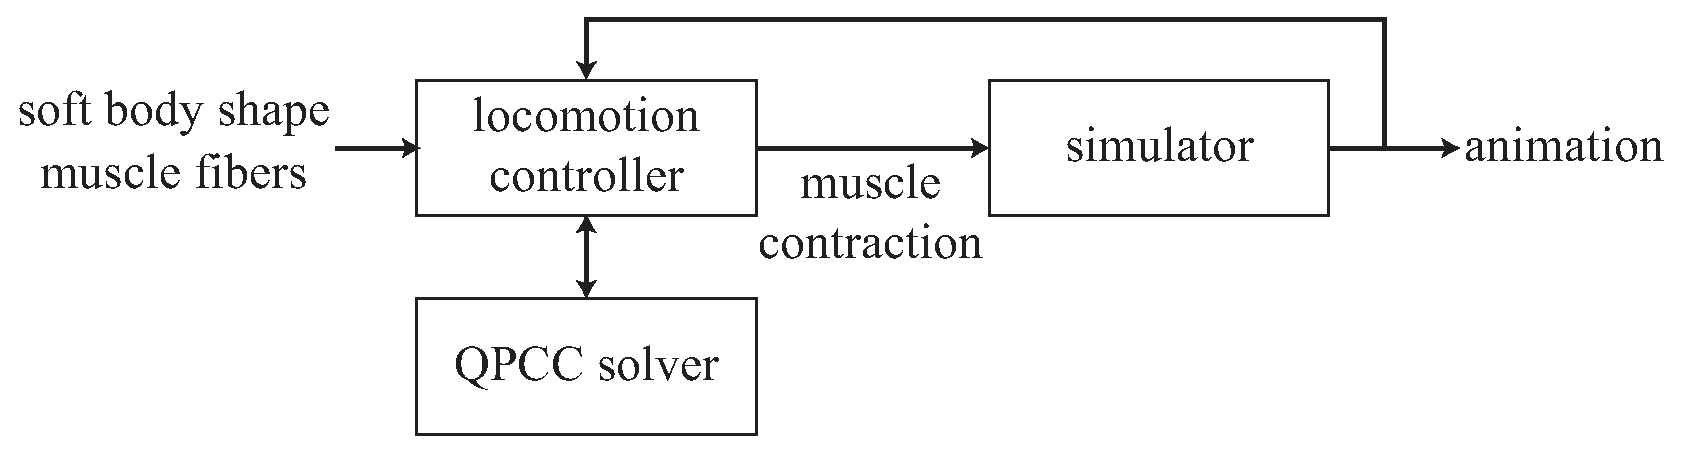
\includegraphics[width=5in]{figures/overview3}
  \caption{Overview of our system.}
  \label{fig:overview}
\end{figure}

We design a wide variety of locomotion controllers for soft bodies,
including balance, walking, crawling, jumping, sliding and rolling.
Given the geometry of a soft-body creature and the
arrangement of its muscle fibers, our controller computes required
muscle contraction to propel the creature to achieve desired
locomotion while maintaining balance. At each time step, the
controller formulates a quadratic program with complementarity
constraints (QPCC) to solve for the optimal muscle contraction under
discretized dynamic equations of motion and frictional contact
constraints. The objective function, assuming a convex quadratic form,
can be designed arbitrarily to address control goals of the desired
locomotion. The optimal muscle contraction is passed to a FEM
simulator to calculate the next state. Figure \ref{fig:overview}
illustrates the main components of our system.

\section{Soft Body Simulation and Modeling}
Before we introduce the control algorithms for locomotion, we first
describe the methods for simulating soft bodies and computing muscle
forces.

\subsection{Finite Element Simulation}
A soft body creature is represented as a tetrahedral mesh and
is simulated using a modified corotational linear FEM
\cite{Muller:2002}. We chose FEM instead of a mass-spring model
because it is difficult to enforce volume preservation for the material with mass-spring systems.
At each time step, the state of the creature,
$\vc{p}$, is computed through numerical integration of the dynamic
equations of motion:
\begin{equation}
\vc{M}\ddot{\vc{p}} = \vc{f}_{x} + \vc{f}_{e}+\vc{f}_{d}+\vc{f}_{m}
\label{eq:softDynamics}
\end{equation}
where $\vc{M}$ is the mass matrix of the discretized soft body and
$\vc{p}$ is the nodal position of the deformed shape. The forces on
the right hand side, $\vc{f}_{x}$, $\vc{f}_{e}$, $\vc{f}_{d}$, and
$\vc{f}_{m}$, indicate external, elastic, damping, and muscle forces
respectively. The external force $\vc{f}_{x}$ includes gravity,
contact force, and user perturbation force.

As notation, when we are specifying a quantity $\vc{q}$
for a single element, we will write this as $\hat{\vc{q}}$.
To compute the elastic force for each element, we adapted the method
suggested by Nesme \etal \cite{NPF05}:
\begin{equation}
\hat{\vc{f}}_e=-\hat{\vc{B}}^T\hat{\vc{D}}\hat{\vc{B}}(\hat{\vc{p}}-\hat{\vc{R}}\hat{\vc{x}})
\end{equation}
where $\hat{\vc{x}}$ indicates the nodal position in the rest shape
and $\hat{\vc{R}}$ transforms the element from the reference
coordinates to the deformed coordinates. $\hat{\vc{B}}$ is the
strain-displacement matrix in the deformed coordinates
and $\hat{\vc{D}}$ is the stress-strain matrix. We use the Poisson ratio 0.45 in $\hat{\vc{D}}$ to make the soft body
nearly incompressible while avoiding locking artifacts \cite{Irving:2007}. Although volume preservation is not enforced strictly, our experiments show that the volume change is below 15\% and is not visually noticeable.
This formulation linearizes the
elastic force around the current deformed shape, rather than around
the rest shape, as used in most FEM implementations. We chose this
formulation because it eliminates ``ghost torques'' caused by the
error of linearization around the rest shape~\cite{NPF05}. When the material is soft or when the deformation is
small, ghost torques do not cause visible artifacts. However, this
formulation is necessary for our case, because soft body locomotion
requires large deformation with relatively stiff materials to support
the weight of the creature.

We assemble the individual stiffness matrices $\hat{\vc{B}}^T\hat{\vc{D}}\hat{\vc{B}}$ for
each element into a large stiffness matrix $\vc{K}$ for the whole
system. The elastic force for all the FEM nodes can be expressed by
$\vc{f}_e=-\vc{K}(\vc{p}-\vc{R}\vc{x})$. For damping force, we use
simple Rayleigh damping model to compute its effect:
$\vc{f}_d=-\vc{C}\dot{\vc{p}}=-(\mu\vc{M}+\lambda\vc{K})\vc{\dot{p}}$. We
set $\mu = 0$ and $\lambda = 0.2$.

\subsection{Muscle Modeling}
We model muscle fibers as polygonal curves with a small number of
segments. Each muscle segment can contract along its current direction, but
it cannot extend or bend. Based on the arrangement of muscle fibers,
we can bundle them into muscle groups. There are three types of
muscles which lead to different control tasks. The \emph{longitudinal
muscles} are linear muscles that extend from one end of the body to the
other end. Their main function is to shorten or bend the body. The
\emph{radial muscles} are a set of short muscles that span a cross-section
of the body. When radial muscles contract, the volume-preserving
nature of the tissue causes the body to elongate. \emph{Helical
muscles} wrap around the body in a helical shape. When a helical muscle
contracts, the body twists.

\ignorethis{These three types of muscles are found in
a variety of soft body creatures and deformable body parts
\cite{Kier:1985}, including worms, elephant trunks, squid tentacles
and human's tongues.}

Muscle contraction induces muscle force on nearby FEM elements. Each
muscle segment is modeled as a spring with a changeable desired
length. The spring force caused by each segment is computed as: $f =
k(l_d - l)$, where $k$ is the stiffness of the muscle fiber, $l_d$ is
the current desired length, and $l$ is the current length of the
segment. We treat $f$ as a virtual force, which is realized by muscle
stress imposed on nearby elements. When a muscle segment contracts
with the virtual force $f$ in the direction of $\vc{d}$ in the
reference coordinates, the effect of contraction is as muscle
stress $\vc{F}$:
\begin{equation}
\vc{F}=\vc{U}\left[\begin{array}{ccc}
f & 0 & 0\\
0 & 0 & 0\\
0 & 0 & 0
\end{array}\right]\vc{U}^T
\end{equation}
where $\vc{U}$ is the matrix that rotates vector $(1, 0, 0)^T$ in the
reference coordinates to be aligned with $\vc{d}$.

Each FEM element may be affected by multiple muscles. The
accumulated muscle stress experienced by an element $i$ is a weighted
sum of all the muscle stresses that have an influence on the element
$i$, denoted in the deformed coordinates of element $i$ as:
\begin{equation}
\hat{\sigma}^i_m=\sum_j w_{ij}\hat{\vc{R}}\vc{F}_j\hat{\vc{R}}^T
\end{equation}
where $w_{ij}$ weighs the influence of muscle fiber $j$ on the element
$i$. The value of $w_{ij}$ is based on the shortest distance
$d_{ij}$, from the muscle fiber to the center of the element in the
reference coordinates. We use a Gaussian kernel as the attenuation
function, $h(d) = \exp(\frac{d^2}{\sigma^2})$, where $\sigma$ is the
variance of the Gaussian function. The influence weight $w_{ij}$ is
defined as
\begin{equation}
w_{ij}=\frac{h(d_{ij})}{\sum_{k\in group(j)}h(d_{ik})}
\label{eq:weight}
\end{equation}
The denominator in eq. (\ref{eq:weight}) normalizes the influence of
muscle fibers within the same group. This normalization allows
different muscle groups, typically with different functionalities,
to exert their influence on the soft body simultaneously.


Once we compute the muscle stress for each element $\hat{\sigma}_m$,
we calculate the force at each face of the element by multiplying
$\hat{\sigma}_m$ with the area-weighted face normal in the deformed
coordinates. Finally, we evenly distribute the force at each face to
the vertices to obtain $\vc{f}_m$ at each node. As a shorthand, we
define a muscle force matrix $\vc{A}$ to express the relation between
the muscle force on each node and the effect of muscle contraction.
\begin{equation}
\vc{f}_m = \vc{A}(\vc{l}_d-\vc{l})
\end{equation}
Note that $\vc{A}\in \mathbb{R}^{3n\times m}$ where $n$ is the number
of nodes in the FEM mesh and $m$ is the number of muscle segments,
which is also the dimension of our control variables.

\subsection{Numerical Integration}
To ensure the stability of our system with large time steps, we use an
implicit integrator to solve the dynamic equations. After substituting
each force terms into eq. (\ref{eq:softDynamics}), we arrive at the following
dynamic equation:
\begin{equation}
\vc{M\ddot{p}}=\vc{f}_x-\vc{K}(\vc{p} -\vc{R}\vc{x}) -
\vc{C}\dot{\vc{p}} +\vc{A}(\vc{l}_d - \vc{l})
\end{equation}
Applying the implicit integrator, we can rewrite the equation as,
\begin{align}
\label{eq:integration}
\widetilde{\vc{M}}\dot{\vc{p}}^{n+1} & = \vc{M}\dot{\vc{p}}^{n} +
\Delta t(\vc{f}^n_{x} - \vc{K}(\vc{p}^n-\vc{R}\vc{x}^n)
+\vc{A}(\vc{l}_d-\vc{l}^n)) \nonumber \\
 & = \widetilde{\vc{f}}^n + \vc{f}_c + \widetilde{\vc{A}} \vc{l}_d \\
 \vc{p}^{n+1}& = \vc{p}^{n}+\Delta t \dot{\vc{p}}^{n+1}
\label{eq:nextState}
\end{align}
where superscript $n$ indicates the discretized time index and $\Delta
t$ is the time step. We define $\widetilde{\vc{M}}=\vc{M}+\Delta t\vc{C}+\Delta t^2\vc{K}$ and $\widetilde{\vc{A}}=\Delta t\vc{A}$, and
single out the contact force as $\vc{f}_c$, which is part of
$\vc{f}_x$ and will be discussed in the next
section. $\widetilde{\vc{f}}^n$ accounts for the remaining terms on
the right hand side of eq. (\ref{eq:integration}).


\section{Locomotion Control}
\label{sec:softControl}

To create functional locomotion using the simulation framework described
in previous section, we need a control algorithm to compute the appropriate
muscle contractions. Our control algorithm formulates an optimization at
each time step to solve for the desired muscle contraction $\vc{l}_d$ that
achieves the control goals subject to physical constraints.

\subsection{Optimization}
We express the objective function in the optimization as a convex
quadratic function of the next state of the soft body: $G(\vc{p}^{n+1})$.
This general function form is sufficient to encode a wide variety of
control goals while retaining convexity of the optimization. Using
eq. (\ref{eq:integration}) and (\ref{eq:nextState}), the optimization
minimizes a reparameterized objective function which implicitly enforces
the equations of motion:
\begin{equation}
\min_{\vc{l}_d} \;\;G(\vc{p}^{n}+\Delta t \vc{\widetilde{M}}^{-1}(\vc{\widetilde{f}}^n +\vc{f}_c + \vc{\widetilde{A}} \vc{l}_d))
\label{eq:objectiveFunction}
\end{equation}
In addition to the objective function, the optimization must satisfy two
constraints. The first constraint enforces the range of muscle
contractions: $0.5 \vc{l}_0 \leq \vc{l}_d \leq \vc{l}_0$, where $\vc{l}_0$ denotes the muscle length at the rest pose. The second constraint enforces valid contact under Coulomb's friction model. We adapt an implicit time-stepping LCP method to regulate contact velocity and contact force, $\vc{f}_c = \vc{N} f_\perp + \vc{D}\vc{f}_\parallel$, where $\vc{N}$ is the unit normal vector, $\vc{D}$ is a set of tangential directions at the contact point, and $f_\perp$ and $\vc{f}_\parallel$ are the magnitudes of normal and tangent forces. The optimization with constraints can be written as
\begin{align}
\label{eqn:softOptimization}
 \min_{\vc{l}_d,\vc{f}_\perp,\vc{f}_\parallel,\lambda} G&(\vc{l}_d,\vc{f}_\perp,\vc{f}_\parallel)  \\
\nonumber  \mathrm{subject\;} &\mathrm{to} \\
\nonumber   &0.5\vc{l}_0 \leq \vc{l}_d \leq \vc{l}_0 \\
\nonumber  &\vc{0} \leq \left[ \begin{array}{c} \vc{f}_\perp \\ \vc{f}_\parallel \\ \lambda \end{array} \right] \perp
 \left[ \begin{array}{c} \vc{N}^T\dot{\vc{p}}^{n+1} \\ \vc{D}^T \dot{\vc{p}}^{n+1} + \vc{E} \lambda \\ \mu \vc{f}_\perp - \vc{E}^T \vc{f}_\parallel \end{array} \right] \geq \vc{0}
\end{align}
where $\vc{\mu}$ is the friction coefficient and $\vc{E}$ is a
block-diagonal matrix of $\vc{e}$, which is a vector of ones. The
complementarity constraints also introduce auxiliary variables
$\lambda$. The physical meaning of $\lambda$ is related to the tangent
velocity of a sliding contact. Please see Anitescu and Portra
\cite{Anitescu:1997} for a complete review of LCP formulation.

A quadratic program with linear complementarity constraints (QPCC) is
well known for its nonconvexity and disjunctive features, which cannot
be solved efficiently by standard nonconvex solvers. Previous work
simplified this problem by assuming that the current contacts will
remain static (the velocities of contact points remain zero) at the next time step. If this assumption is not
consistent with the simulated result, the controller will try to
correct it at the next time step. In soft body control, assuming
static contacts is too restrictive and significantly reduces the
effectiveness of the controller. As a result, we cannot drop the
complementarity constraints in the optimization. We will introduce a
new iterative solver to QPCC for contact modeling in Chapter
\ref{sec:QPCC}.

\subsection{Low-level Controllers}
\label{sec:controller}
We develop three types of low-level control mechanisms by formulating different
objective functions $G(\vc{l}_d, \vc{f}_\perp, \vc{f}_\parallel)$ in
eq. (\ref{eqn:softOptimization}). In Chapter \ref{sec:softResults}, we
demonstrate that these three basic mechanisms can be combined to
design fundamentally different locomotion controllers.

\paragraph{Momentum control.}
Regulating momentum is of paramount importance for biped balance and
locomotion. Previous work \cite{Macchietto:2009} has
demonstrated that controlling the linear momentum relative to the
contact support is a simple but very effective balance strategy. We
use the following objective function to regulate the linear momentum, $\vc{L}$.
\begin{equation}
G(\vc{l}_d, \vc{f}_\perp, \vc{f}_\parallel) = \| \dot{\vc{L}}(\dot{\vc{p}}^{n+1}, \dot{\vc{p}}^n) - \bar{\dot{\vc{L}}} \|^2
\end{equation}
The desired change of linear momentum $\bar{\dot{\vc{L}}}$ is defined as
\begin{equation}
\bar{\dot{\vc{L}}} = m K_p (\bar{\vc{c}} - \vc{c}^n) - K_d \vc{L}^n
\end{equation}
where $m$ is the mass of the creature and $\vc{c}$ is the center of
mass (COM) position. $K_p$ and $K_d$ are the stiffness and damping
coefficients for the feedback control. For balance control, the
desired COM position $\bar{\vc{c}}$ is computed based on the center of
the contact support area.

Angular momentum also plays an important role in balance. For soft
body creatures, controlling angular momentum is also essential to
rolling motion.
\begin{equation}
G(\vc{l}_d, \vc{f}_\perp, \vc{f}_\parallel) = \| \dot{\vc{H}}(\dot{\vc{p}}^{n+1}, \dot{\vc{p}}^n, \vc{p}^n) - \bar{\dot{\vc{H}}} \|^2
\label{eqn:angular}
\end{equation}
where $\bar{\dot{\vc{H}}}$ denotes the target value for the change of
angular momentum and $\dot{\vc{H}}$ computes the change of angular
momentum at the next state.

\paragraph{Base control.}
In addition to controlling the momentum, we can increase the contact area
to provide a wider range of support to the COM. This balance strategy
is particularly interesting for soft bodies. By squashing and
stretching its entire body, a soft body creature can adjust its base
area at will to maintain balance. We define an objective function that
controls the projected base area $A$ by matching its change rate to
a desired rate $\bar{\dot{A}}$:
\begin{equation}
G(\vc{l}_d, \vc{f}_\perp, \vc{f}_\parallel) =
\| \dot{A}(\dot{\vc{p}}^{n+1}, \vc{p}^n)  - \bar{\dot{A}}\|^2
\end{equation}
We compute $A$ by projecting a defined base area to the ground surface with
normal vector $\vc{n}$:
\begin{equation}
A = \frac{1}{2} \sum_i \left( (b_i - a_i) \times (c_i - a_i) \right)^T \vc{n}
\end{equation}
where index $i$ loops over all triangles in the base area, and $a_i$,
$b_i$, and $c_i$ are the vertices of the $i$th triangle. When
computing $\dot{A}$, we evaluate the velocity terms at
$\dot{\vc{p}}^{n+1}$ and the position terms at $\vc{p}^n$. This
approximation has negligible effect on accuracy, but keeps our
objective function convex.

\paragraph{Position and velocity tracking.}
Direct control of a Cartesian position or velocity is also an effective
way to regulate locomotion. For example, tracking the trajectory of a foot
is essential for producing a walking gait. The following objective function minimizes the distance between a particular body point at the next time step and a target Cartesian point $\bar{\vc{p}}$
\begin{equation}
G(\vc{l}_d, \vc{f}_\perp, \vc{f}_\parallel) = \| f(\vc{p}^{n+1}) - \bar{\vc{p}} \|^2
\label{eqn:positionTracking}
\end{equation}
where $f$ is a function that selects a node from $\vc{p}^{n+1}$. If we redefine $f$ as a function that computes the COM, eq. (\ref{eqn:positionTracking}) can be used to track the COM. Likewise, we can track the relative position of two body points by replacing $f(\vc{p}^{n+1})$ with $f_1(\vc{p}^{n+1}) - f_2(\vc{p}^{n+1})$, where $f_1$ selects the first node and $f_2$ selects the second node from $\vc{p}^{n+1}$. We can also use a similar objective function to track velocity.
\begin{equation}
G(\vc{l}_d, \vc{f}_\perp, \vc{f}_\parallel) = \| f(\dot{\vc{p}}^{n+1}) - \bar{\dot{\vc{p}}} \|^2
\label{eqn:velocityTracking}
\end{equation}


\section{QPCC for contact modeling}
\label{sec:QPCC}

The control framework described in Chapter \ref{sec:softControl} requires
an efficient QPCC solver that can handle $50$ to $100$ complementarity
variables. Solving QPCC in general is difficult due to the presence of
the linear complementarity constraints. A na\"{\i}ve way to solve QPCC is
to evaluate all the valid combinations of the complementarity
constraints and output the minimizer. This exhaustive method is
guaranteed to find the global minimum. However, the computational time
grows exponentially with the number of variables involved in the
complementarity constraint. In our control problem, we have 10
variables for each contact point (one for $f_\perp$, eight for
$\vc{f}_\parallel$ and one for $\lambda$). Thus, a few contact points
alone will render the exhaustive method computational impractical.

We propose a more efficient way to solve a QPCC for contact problems, such as eq. (\ref{eqn:softOptimization}). Our iterative QPCC solver starts with an initial guess, which is a set of linear constraints that are compatible with the complementarity conditions. For the initial guess, we manually set some elements of $\vc{f}_\perp$, $\vc{f}_\parallel$, and $\lambda$ to be zero and their complementary pairs to be nonnegative, in a way that the state of those variables has a physical meaning. For example, if we assume all contact points are static, we arrive at the following convex QP:
\begin{align}
\min_{\vc{l}_d,\vc{f}_\perp,\vc{f}_\parallel,\lambda} G&(\vc{l}_d,\vc{f}_\perp,\vc{f}_\parallel) & \label{eqn:initialGuess} \\
\mathrm{subject\;} &\mathrm{to} & \nonumber\\
 & 0.5\vc{l}_0 \leq \vc{l}_d \leq \vc{l}_0 & \nonumber \\
 & \vc{0} \leq \vc{f}_\perp, & \vc{N}^T\dot{\vc{p}}^{n+1} = \vc{0} \label{eqn:initialGuess1}\\
 & \vc{0} \leq \vc{f}_\parallel, &  \vc{D}^T \dot{\vc{p}}^{n+1} + \vc{E} \lambda = \vc{0} \label{eqn:initialGuess2}\\
 & \vc{0} = \lambda, & \mu \vc{f}_\perp - \vc{E}^T \vc{f}_\parallel \geq \vc{0} \label{eqn:initialGuess3} \\
 \nonumber
\end{align}


After solving the above QP, we examine the complementarity conditions
at the minimizer. We identify those inequality constraints that reach
their boundary at the minimizer as candidates for pivoting. Our
algorithm pivots one of those candidates at a time. That is, we set
the candidate to equality constraint and flip its complementary
counterpart from equality to inequality. By pivoting the
complementarity constraints, we formulate a new QP with a set of different
linear constraints and we solve for the minimizer for this new
QP. We repeat this process until all the candidates reach the local
minimum of the QPCC, \ie until we encounter a minimizer that lies in the
interior of the feasible region. The candidate that yields the best
local minimum is returned as the solution of the QPCC. Our QPCC solver
explores the nonconvex feasible region based on the following
heuristics: Each pair of the complementarity constraints defines a
feasible region formed by two intersecting half-hyperplanes. If a minimizer hits the boundary of the half-hyperplane, exploring the other
half-hyperplane might give a better minimizer. Figure \ref{fig:QPCC}
shows a two dimensional example.

\begin{figure}[!b]
  \centering
  \includegraphics[width=5in]{figures/QPCC.eps}
  \caption{A simple 2D QPCC example. The complementarity constraints are $0\leq x \perp x-y-2 \geq 0$. (a) The feasible region lies in two intersecting half-hyperplanes, shown as two black line segments. (b) With the initial guess of $x=0$ and $x-y-2\geq 0$, the minimizer, shown as an orange dot, is located at the boundary of the inequality constraint. (c) After pivoting the constraint, setting $x\geq 0$ and $x-y-2=0$, we find a better minimizer (global minimizer in this simple case).}
  \label{fig:QPCC}
\end{figure}

Our algorithm further exploits the structure of a contact problem to
improve the performance. Instead of arbitrarily selecting a candidate
to pivot, we can group the complementarity constraints according to
their physical meaning and pivot a whole group together. There are
three different situations for each contact point: static, sliding and
contact breakage. Pivoting constraints in eq.
(\ref{eqn:initialGuess1}) indicates a switch between a static (or a
sliding) contact and contact breakage.  Pivoting constraints in
eq. (\ref{eqn:initialGuess2}) and (\ref{eqn:initialGuess3})
indicates a switch between static and sliding contact. For example, if
$\vc{f}_{\perp}(i)=0$ is the result of solving the QP (eq.
(\ref{eqn:initialGuess})), it implies that breaking $i$th contact point
might lead to a better minimizer for the QPCC. The solver will pivot
the corresponding constraints: $\vc{f}_{\perp}(i) \geq 0 \rightarrow
\vc{f}_{\perp}(i) = 0$ and $(\vc{N}^T\dot{\vc{p}}^{n+1})(i) = 0
\rightarrow (\vc{N}^T\dot{\vc{p}}^{n+1})(i) \geq 0$. The new QP will
be solved subsequently. Conversely, when a free point restores a static
contact, we apply the opposite pivoting.

If a friction cone condition (eq. (\ref{eqn:initialGuess3})) for the
$i$th contact point needs to be pivoted, this implies that the $i$th contact point is about to slide and switching it from static to sliding might lead to a better minimizer. The solver then changes the inequality constraint $(\mu \vc{f}_{\perp} - \vc{E}^T \vc{f}_{\parallel})(i)\geq 0$ to equality and changes the corresponding equality constraint $\lambda(i)=0$ to inequality. In addition, we need to pivot some constraints in eq. (\ref{eqn:initialGuess2}) to specify the direction of the sliding contact, which can be estimated using the static friction from the current minimizer. We project this static friction force to each of the tangential direction of the $i$th contact point $\vc{D}(i)$ and find the two directions (the $m$th and $n$th direction in $\vc{D}(i)$) that have the largest magnitude. The sliding force direction is estimated to be along the convex combination of $m$th and $n$th directions. We pivot the constraints in the following way,
\begin{align}
& \vc{f}_{\parallel}(i, m)\geq 0, \;\;\; (\vc{D}^T \dot{\vc{p}}^{n+1} + \vc{E} \lambda)(i, m) = 0 \nonumber \\
& \vc{f}_{\parallel}(i, n)\geq 0, \;\;\; (\vc{D}^T \dot{\vc{p}}^{n+1} + \vc{E} \lambda)(i, n) = 0\nonumber \\
& \vc{f}_{\parallel}(i, j) = 0, \;\;\;(\vc{D}^T \dot{\vc{p}}^{n+1} + \vc{E} \lambda)(i, j) \geq 0, ~~\forall j \neq m, n\nonumber
%(\vc{D}^T \dot{\vc{p}}^{n+1} + \vc{E} \lambda)(i, m) = 0 &
%(\vc{D}^T \dot{\vc{p}}^{n+1} + \vc{E} \lambda)(i, n) = 0 & \nonumber \\
%(\vc{D}^T \dot{\vc{p}}^{n+1} + \vc{E} \lambda)(i, j) \geq 0, & ~~\forall j \neq m, n \nonumber\\
\label{eqn:staticSlidePivot}
\end{align}
where $\vc{f}_{\parallel}(i, j)$ is the magnitude of the friction force
along the $j$th direction for the $i$th contact
point\footnote{$\vc{f}_{\parallel}(i, j)$ is actually the $(i\cdot N+j)$th
element of $\vc{f}_{\parallel}$ assuming that $N$ tangential directions
are used for the linearized friction cone for each contact point.}. For
the special case, where the friction force is exactly along the $m$th (or
$n$th) direction, we only pivot the complementarity constraints involving
the $m$th (or $n$th) direction. For a switch between sliding to static
contact, we use the same pivoting mechanism but pivot the constraints the
opposite way.

Instead of searching exhaustively in the feasible region of the QPCC, our
solver systematically explores the feasible region based on the above
mentioned heuristics. Although the objective value is not guaranteed to
decrease monotonically, our experiments show that the objective value
decreases drastically within a small number of iterations. The minimizer
found by our solver is, in all the experiments, significantly closer to
optimal than the one solved under the static contact assumption. We report the
results of the experiments in Chapter \ref{sec:softEvaluation}.

\paragraph{Implementation.}
Our solver requires a feasible initial guess. We can use the trivial solution under static contact assumption (eq. (\ref{eqn:initialGuess})) as an initial guess, or the solution from the previous QPCC when it is available (warm start). Occasionally, they might result in an infeasible QP. For those cases, we assume the same muscle activation as in last time step, remove the objective function and muscle length constraints from eq. (\ref{eqn:softOptimization}) and solve a pure LCP. The contact situation from the LCP solution is then used as the initial guess for the QPCC.

We implement the QPCC solver using a graph expansion algorithm (See Appendix \ref{chapter:AppendixA} for details). Each
QP with linear constraints is a node in the graph. We visit each node
twice, starting from the initial guess as the root. In the first
visit, we solve the QP, assign the objective value to the
node, and store the set of candidates to be pivoted. After first
visit, we push the node into a priority queue based on its objective
function value. A node is visited the second time when it is at the
top of the queue. In the second visit, we pivot the constraints from
its candidate set. Each pivot generates a child node. We discard the
child node if it already exists in the current graph. If the child
node is new, we visit the node for the first time and push it into the
queue. The second visit is completed when all the constraints in the
candidate set are pivoted. We then pop the next node in the queue and
repeat this process. The algorithm terminates when the priority queue
is empty or the number of visited nodes exceeds a threshold. The final
solution is the best minimizer found so far by the QPCC solver.

\section{Results}

\label{sec:softResults}
\begin{figure*}[ht]
\centering
\includegraphics[width=\textwidth]{figures/HSwing.eps}
\caption{An H-shaped soft body character does its morning exercises by swinging its body from one side to the other.}
\label{fig:HSwing}
\end{figure*}

\begin{figure*}[ht]
\centering
\includegraphics[width=\textwidth]{figures/IBalance.eps}
\caption{An I-shaped soft body character tries to maintain balance under
perturbation by regulating its momenta, widening its base and lowering its center of mass.}
\label{fig:IBalance}
\end{figure*}

In this section we describe the results of our soft body locomotion
controllers. Please see the video\footnote{http://dl.dropbox.com/u/36899427/softbodylocomotion.mp4} to watch the locomotion
animations. Our system is implemented in C++, and we generated the
tetrahedral mesh for FEM simulation using TETGEN \cite{Si:2006}. We
used the GPU to create layered depth figures for collision detection,
and we used contact patches (multi-resolution volume contact)
\cite{Allard:2010} instead of points as the contact primitives. For
each contact patch, we use eight tangential directions to linearize
the friction cone, which provides sufficient accuracy while keeping the QPCC tractable. The examples were run on a workstation with a
2.26GHz CPU and 4GB of memory. All the data of our locomotion
examples are summarized in Table~\ref{table:data}.

\begin{table}[!b]
  \centering
   \caption{Parameters and performance of examples. \# tets: the number of
  elements in the FEM simulation. \# dofs: the number of muscle degrees of
  freedom for the soft body. Sim time, opt time and total time are the average simulation,
  optimization and total time (in second) per frame.}
\begin{tabular}{|c|c|c|c|c|c|c|}
\hline
examples & \# tets & \# dofs  & \# contact     & sim  & opt & total\\
         & & & patches & time & time & time\\
 \hline
exercise(H) & 1901 & 52  & 4 & 0.54 & 0.05 & 0.59\\
balance(I)  & 1066 & 48  & 4 & 0.31 & 0.28 & 0.59\\
slide(F)    & 705  & 48  & 4 & 0.25 & 0.23 & 0.48 \\
jump(I)     & 1066 & 104 & 4 & 0.33 & 0.48 & 0.81 \\
jump(T)     & 1219 & 51  & 4 & 0.63 & 0.30 & 0.93 \\
roll(O)     & 911  & 40  & 6 & 0.26 & 0.18 & 0.44\\
crawl(I)    & 620  & 26  & 8 & 0.18 & 0.24 & 0.42\\
walk(X)     & 1128 & 112 & 4 & 0.54 & 0.70 & 1.24\\
\hline
 \end{tabular}
 \label{table:data}
 \end{table}

We design many different shapes of the soft body characters, all of
which are chosen from the English alphabet. Figure~\ref{fig:HSwing} shows
an H-shaped character doing morning exercises. The character is designed
with four longitudinal muscles and one radial muscle for each
leg (Figure~\ref{fig:muscles}a). It is animated by specifying the
trajectory of the desired center of mass (COM), which is moved left/right
by a sine function. We use the position and velocity tracking controller
from Chapter \ref{sec:controller} to track the desired COM. Note that when
the ``H'' swings left, its right side elongates and gets thinner while the
left side shortens and becomes fatter due to the volume preservation. This
animation clearly exemplifies the principle of \emph{squash and stretch}.

\paragraph{Balance.} We design an I-shaped character
(Figure~\ref{fig:IBalance}) to demonstrate static balance.  We gave
the character four longitudinal muscles that allow it to bend in any
direction.
This character is perturbed by a large force exerting at
its head, and it attempts to recover its balance. Static balance of
the ``I'' turns out to be one of the most difficult task among all our
examples. The geometry of the letter ``I'' does not have limbs or
other appendages to help it regulate the linear and angular
momentum. The squishy body and lack of skeletal support make the task
even more challenging. In addition to momentum control for balance,
which is not enough to prevent the ``I'' from falling, we exploit the
advantage of its flexible body shape.  We include a term in the
objective function that encourages it to widen its support base.  With
this wider base, the contact area is increased and the COM is lowered,
which helps with the balance task. Without our QPCC solver, base widening would be difficult
to achieve, because it requires frequent switching from static to sliding contacts.
In addition, we observe that right
after the perturbation, half of the base is lifted from the ground and
the contact area concentrates on the rim of the base to provide the maximum
amount of angular momentum to combat the perturbation. It is similar
to a human lifting his or her heels and using only toes to balance
when pushed from behind. This natural contact strategy
emerges automatically from our QPCC solution.  To compare our
QPCC solver and a more commonly used QP solver with linear
constraints, we produced two animation sequences of the ``I''
balancing, one with each solver.  QPCC produced natural and effective
balance motions, including changing contact situation, lowering the
COM, widening the base and regulating momentum. In contrast, the QP
solver (which only allows for static contact constraints) resulted in a falling motion.

\begin{figure*}[t]
\centering
\includegraphics[width=\textwidth]{figures/FBalance.eps}
\caption{An F-shaped soft body character maintains balance under a persistent and continuously increasing pulling force on a slippery surface. It actively leans backward to avoid tipping over.}
\label{fig:FBalance}
\end{figure*}

\begin{figure*}[t]
\centering
\includegraphics[width=\textwidth]{figures/IJump.eps}
\caption{An I-shaped soft body character squashes and stretches its whole body to jump forward.}
\label{fig:IJump}
\end{figure*}


\begin{wrapfigure}{r}{0.2\textwidth}
\center
%\vspace{-30pt}
\hspace{-30pt}
\includegraphics[width=0.2\textwidth]{figures/SlideController.eps}
\end{wrapfigure}

\paragraph{Sliding.} In the example of Figure~\ref{fig:FBalance},
instead of applying a perturbation force that lasts for a short time,
we exert an continuously increasing pulling force on the ``F'' standing on
a slippery surface. We design a sliding balance controller for this
special balance task. The controller estimates the optimal relative
position between the center of base (COB) and the COM such that the
total angular momentum is zero. We use the position and tracking controller to track the optimal COB. The sliding balance controller also benefits from our QPCC
solution since planning the movement of the COB involves planing the
change of contact situation (from static to sliding).  We instrument the vertical stroke of the ``F'' with four
longitudinal muscles. Even though no muscle resides in the horizontal
parts of this character, the two horizontal strokes are still
influenced by the muscles in the main body. The first sequence of
sliding balance in the video shows that the ``F'' leans left while it is
dragged towards the right.  As the drag force increases, the ``F'' leans more
and more to prevent from tipping over. The second sequence shows the
sliding motion when it is dragged to the left. The sliding motion is
different from the first one due to the asymmetry of the body
shape. The elongation and oscillation of the top stroke of the ``F''
demonstrates the animation principle of \emph{follow through}. In the
third sequence, we applied the sliding balance controller 0.3 second
after the start of dragging to delay the character's
response time. The slow response of the ``F'' makes it difficult to
maintain the optimal COB-COM relative position. It struggles to keep
balance by constantly switching between sliding and breaking contact
(small jumps), and eventually it manages to balance.  These changes of
contact, due to the QPCC solver, makes the controller more robust and
the soft body character more lifelike.

\begin{figure*}[t]
\centering
\includegraphics[width=\textwidth]{figures/TTwist.eps}
\caption{A T-shaped soft body character twists using helical muscles when jumping.}
\label{fig:TJump}
\end{figure*}

\begin{figure*}[t]
\centering
\includegraphics[width=\textwidth]{figures/XWalk.eps}
\caption{An X-shaped soft body quadraped walks by slowly lifting and moving one foot at a time.}
\label{fig:XWalk}
\end{figure*}


\begin{figure}[!b]
\centering
\includegraphics[width=3in]{figures/muscles2.eps}
\caption{Examples of the muscle fiber designs for various soft body characters. Each curve inside the character represents a muscle fiber, which consists of a number of independently contracting degrees of freedom.}
\label{fig:muscles}
\end{figure}

\paragraph{Jumping.} Jumping is an visually interesting form of
locomotion for soft body characters as it is often seen in cartoons
and animations. Our jumping controller consists of three separate
controllers for takeoff phase, airborne phase, and landing
phase. During the takeoff phase, we use the position and velocity
tracking controller to follow a desired trajectory of the COM. We also
set $\bar{\dot{H}}=\vc{0}$ to the angular momentum controller, which
prevents large rotation at takeoff.  During the airborne phase, we control the relative
position between the COB and COM. Extending the COB towards the
direction of jumping helps the character balance after landing. Upon
landing, we switch to the static balance controller.
Figure~\ref{fig:IJump} shows a forward jumping motion of the same
character ``I'' with a slightly different fiber arrangement.
We add four more longitudinal muscles and one radial muscle to help it with this highly dynamic motion.
Another sequence in the video shows successive jumps in place.
Figure~\ref{fig:TJump} demonstrates
a twist jump and the use of helical muscles
(Figure~\ref{fig:muscles}b).  Before the ``T'' takes off, we set
$\bar{\dot{H}}=(0, 600, 0)^T$ to make it twist its body.

\paragraph{Rolling.} In the video, we also demonstrate
locomotion by rolling. We designed an O-shaped character with two
loops of muscle fibers arranged as two concentric circles
(Figure~\ref{fig:muscles}c). Each fiber consists of 20 independent segments, which allow
the ``O'' to control its shape locally. The rolling motion is initiated by moving the COM in front of the contact patches. We use the angular momentum control to
make it roll. In the first animation, we set the desired
change of angular momentum $\bar{\dot{H}}$ to be $(0, 0, -200)^T$ in
the first 90 frames. We observe that the character actively changes its
shape by shifting its weight to the right in order to roll. After the character starts rolling,
we disable the controller
and simulate the passive rolling. The character recovers to its
original symmetric rounded shape and the rolling stops after a while
due to friction. In the second animation, we compare our result with
the motion solved by a QP using the static contact assumption.  When we only
allow static contact, the ``O'' never begins rolling because this
motion requires the character to break contact, which is prohibited by the static contact assumption (eq.~(\ref{eqn:initialGuess1})).  The third sequence
shows that the ``O'' starts to roll right, deaccelerates, stops
and rolls to the left by applying a time varying $\bar{\dot{H}}$ to
the controller.

\paragraph{Crawling.} Crawling is often used by soft body creatures in
nature, such as earthworms.  To demonstrate crawling motion, we
flatten the ``I'' and lay it down on the ground. In addition to the
four longitudinal muscles run along four sides of the body, we add
another radial muscle in the middle of its body to facilitate the
elongation of the body. We specify the trajectory of its four
corners for the crawling motion; the back of the character moves while
it is contracting, and the front moves when it elongates.  We use the
position and velocity tracking controllers to match the trajectory. As
Miller noted, such creatures have oriented scales that result in
anisotropic friction~\cite{Miller:1988}.  We incorporate just such an
anisotropic friction into our contact model by modifying the contact
force to $\vc{f}_c=\vc{N}f_\perp+\vc{DS}\vc{f}_\parallel$, where
$\vc{S}$ is a diagonal scaling matrix that modulates the frictional
force according to the direction of motion. We set the friction
coefficient in the backward direction to be 10 times larger than all
other directions. In the video, we demonstrate the
earthworm style of crawling. The whole body of the character lies flat
on the ground at all times and it moves forward by repeatedly
shortening and elongating its body. The contact strategy of this form
of crawling is complex. During shortening, the front end of the body
is in static contact while the rear end is sliding forward. During
elongating, the front end switches to sliding contact while the rear
end switches to static contact. It is challenge to capture this
complex contact strategy using the traditional control mechanism, but
it emerges automatically by solving QPCC.

We also demonstrates an inchworm style of crawling, using the same
body geometry and muscles as the earthworm. For this style of motion,
the body bends upward periodically at the middle and the contacts
mostly concentrate at the two ends of the body. We achieve this effect
using the same controller as in the earthworm style crawling with an
additional constraint that the upper longitudinal muscle cannot
contract.  While other muscles contract to tracking the trajectory,
the asymmetric muscle contractions bend the body upwards naturally.

\paragraph{Walking.} Figure~\ref{fig:XWalk} demonstrates the walking
motion of an X-shaped quadruped. We instrument four longitudinal
muscles and two radial muscles for each limb of the ``X''
(Figure~\ref{fig:muscles}d) and specify the trajectories for all of
its four feet. We apply the position and velocity tracking controller, to track this the walking motion.
The first sequence in the video shows a careful and slow gait that moves only one
foot at a time. The second walking sequence shows a faster walking
gait by simultaneously lifting and moving two feet at a time. The
breaking of contact when a foot lifts from the ground is handled
automatically by the QPCC solver.

\section{Discussion}
\label{sec:softEvaluation}

We have presented a system for animating soft body characters, with a
particular emphasis on locomotion.  Key aspects of our approach include
the coordinated deformation of groups of finite elements using virtual
muscle fibers, the specification of high-level goals by the animator, and
the use of a new solver that handles static, sliding and breaking contact
cases.  Our system allows us to create soft body characters that
demonstrate a variety of locomotion behaviors, including crawling,
hopping, walking, sliding and rolling.  Our characters move in an organic
manner, and they follow the animation principles of anticipation,
squash-and-stretch, and follow through.

One important contribution of this chapter is the formulation of QPCC and its solver.
QPCC is an NP-hard problem \cite{Braun:2005} and our method provides an effective heuristic.
To evaluate our QPCC solver, we tested it on $10$
QPCC problems with 98 variables and 40 pairs of linear complementarity
constraints. We compared our solutions (QPCC in Table~\ref{tab:qpcc}) with the ground truth, as well
as with the solutions based on the static contact assumption (QP in Table~\ref{tab:qpcc}). The
ground truth is computed by an exhaustive search, \ie, solving a QP
for every combination of complementarity variables and selecting the one
with the lowest objective value. We evaluated our results using a ``gap
ratio'', defined as the ratio of difference in the optimal value between
our solver and the ground truth, to the difference in the optimal value
between the static contact assumption and the ground truth. On average
of $10$ problems, the gap ratio is $6.29$, indicating that our solver
yields solutions $6.29$ times closer to the ground truth than the
solutions based static contact assumption. We also selected the best
case and the worst case according to the gap ratio and reported them
in Table \ref{tab:qpcc}.
\begin{table*}
  \centering
   \caption{The results of the numerical experiments of the QPCC solver. }
\begin{tabular}{|l|r|r|r|r|r|r|r|r|r|r|}
\hline
&\multicolumn{3}{|c|}{QPCC} & \multicolumn{3}{|c|}{QP}  & \multicolumn{3}{|c|}{Ground Truth} \\ \hline
& Avg & Best & Worst & Avg & Best & Worst & Avg & Best & Worst \\ \hline
Obj Value & 1483.2 & 21.8 & 697.9 & 5222.8 & 2072.0& 1246.9 & 772.9 & 0.0 & 0.0 \\ \hline
\#Iterations & 17 & 3 & 31 & 1 & 1 & 1 & 10000 & 10000 & 10000 \\
\hline
\end{tabular}
 \label{tab:qpcc}
\end{table*}
Although the empirical results showed that our QPCC solver can
effectively solve contact resolution problem and balance between the
quality of solution and computational time, the QPCC solver does not
guarantee finding the minimizer in polynomial time. In the
worst case, it takes the same amount of time as the exhaustive search
to find the global minimizer.

Our system has a few limitations.  The
optimization scheme described in Chapter \ref{sec:softControl} only
optimizes the control variables for the next time step. This type of
greedy algorithm sometimes leads to unnaturally large muscle contraction or
discontinuities in motion. For example, the rolling ``O'' demo in the
video exhibits some unnatural vibration. Furthermore, the greedy algorithm prevents us
from simulating anticipatory behaviors in motion. For example, we were
not able to develop a ``cartwheel'' controller for the I-shaped
character because a natural and stable cartwheel motion requires
optimizing a long-window of trajectory. This issue can potentially be
solved by implementing long-horizon optimization or model predictive
control methods.

One of the issues that we hope to explore in the future is to expand
our solution techniques to handle longer-term goals that cannot be
reached using our current optimization method. In this work, all muscles are manually designed. We would like to develop an automatic muscle design algorithm to incorporate more sophisticated muscle structures.
We would also like to
investigate muscle design for chunkier creatures. For example, it is
not immediately obvious how muscle fibers should be arranged for the
Stanford Bunny. Another possibility is to note that in our current
system, we only use contracting muscle fibers in order to change the
shape of our characters.  It would be interesting to explore other
forms of shape control, such as elongating muscles or sheets of
virtual muscles.  Another possible direction would be to explore the
animation of soft body characters in water, since many real soft-body
creatures live in an aquatic environment.  Finally, our current
animator controls are provided as program modules, and an easier way
to use them would be to plug them together using a graphical user
interface.

\chapter{Locomotion with a Passive Mechanical Device}
\section{Motivation}

The bicycle was voted as the best invention since the 19th century \cite{BBC2005} because it is an inexpensive, fast, healthy and environmentally friendly mode of transportation. However, riding a bicycle is nontrivial due to its inherently unstable dynamics: The bike will fall without forward momentum and the appropriate human control. Getting onto the bike, balancing, steering and riding on bumpy roads all impose different challenges to the rider. As one important child development milestone, learning to ride a bicycle often requires weeks of practice. We are interested to find whether it is possible to use a computer to mirror this learning process. In addition to the basic maneuvers, the most skillful riders can jump over obstacles, lift one wheel and balance on the other, and perform a large variety of risky but spectacular bicycle stunts. Performing stunts requires fast reaction, precise control, years of experience and most importantly, courage, which challenges most people. Can we design an algorithm that allows computers to automatically learn these challenging but visually exciting bicycle stunts?

Designing an algorithm to learn to ride a bicycle presents unique challenges. Riding a bicycle involves complex interactions between a human rider and a bicycle. While the rider can actively control each joint, the bicycle is a passive system that can only be controlled by the human rider. To control a single degree of freedom (DOF) of a bicycle, coordinated motions of multiple DOFs of the rider are required. Moreover, the main difficulty in locomotion is to control an under-actuated system by exploiting external contact forces. Manipulating contact forces on a bicycle is indirect. All of the rider's control forces need to first go through the bicycle dynamics to affect the ground reaction forces and vice versa. This extra layer of bicycle dynamics between the human control and the contact forces adds another layer of complexity to the locomotion control. Balance on a bicycle is challenging and it is different from balance when standing or walking. While a human can stand stably due to the large contact area of the feet, a static bicycle cannot stay upright due to its narrow tires. Humans can balance during walking by planning and changing their foot placement. In contrast, the bike rider cannot abruptly change the contact position, which can only be changed gradually through steering. The limited range of human motion on a bicycle makes balance even harder. When the character's hands are constrained to hold the handlebar and their feet are on the pedals, the character loses much of the freedom to move various body parts. He or she cannot employ ankle or hip postural strategies or wave their arms to effectively regulate the linear and the angular momenta.

Balance during bicycle stunts is far more challenging than normal riding. As a stunt example that illustrates the balance issues we plan to tackle, consider a bicycle endo (bottom-left image of Figure~\ref{fig:teaser3}), in which the rider lifts the rear wheel of the bicycle and keeps balance on the front wheel. In this pose, the rider encounters both the longitudinal and lateral instabilities. The small contact region of one wheel and the lifted center of mass (COM) due to the forward leaning configuration exacerbate the balance problem. Furthermore, the off-the-ground driving wheel makes any balance strategies that involve acceleration impossible. The unstable configurations and the restricted actions significantly increase the difficulty of balance during a stunt.

This paper describes a complete system for controlling a human character that is riding a bicycle in a physically simulated environment. The system consists of two main components: simulating the motion and optimizing the control policy. We simulate the bicycle and the rider as an articulated rigid body system, which is augmented with specialized constraints for bicycle dynamics. The second component provides an automatic way to learn control policies for a wide range of bicycle maneuvers. In contrast to many optimal control algorithms that leverage the dynamics equations to compute the control signals, we made a deliberate choice not to exploit the dynamics equations in our design of the control algorithm. We believe that learning to ride a bicycle involves little reasoning about physics for most people. A four-year-old can ride a bicycle without understanding any physical equations. Physiological studies show that learning to ride a bicycle is a typical example of implicit motor learning \cite{Chambaron2009}, in which procedural memory guides our performance without the need for conscious attention. Procedural memory is formed and consolidated through repetitive practice and continuous evolution of neural processes. Inspired by the human learning process, we formulate a partially observable Markov decision process (POMDP) and use policy search to learn a direct mapping from perception to reaction (procedural memory).

Both prior knowledge of bicycle stunts and an effective searching algorithm are essential to the success of policy search. After studying a variety of stunts, we classify them into two types. We apply feed-forward controllers for the \emph{momentum-driven} motions and feedback controllers for the \emph{balance-driven} ones. We study videos of stunt experts to understand their reactions under different situations and used this information to design the \emph{states} and the \emph{actions} of our controllers. We employ a neural network evolution method to simultaneously optimize both the parametrization and the parameters of the feedback controllers. The way we incorporate the prior knowledge into our system and the effective evolutionary method are both essential to the success of policy search.

We evaluate our system by demonstrating a human character riding different types of bicycles and performing a wide variety of stunts (Figure \ref{fig:teaser3}). We also evaluate the importance of optimizing the parametrization of a policy. We share our experiences with different reinforcement learning algorithms that we have tried throughout this research project.


\section{Overview}
\begin{figure}[!t]
  \centering
  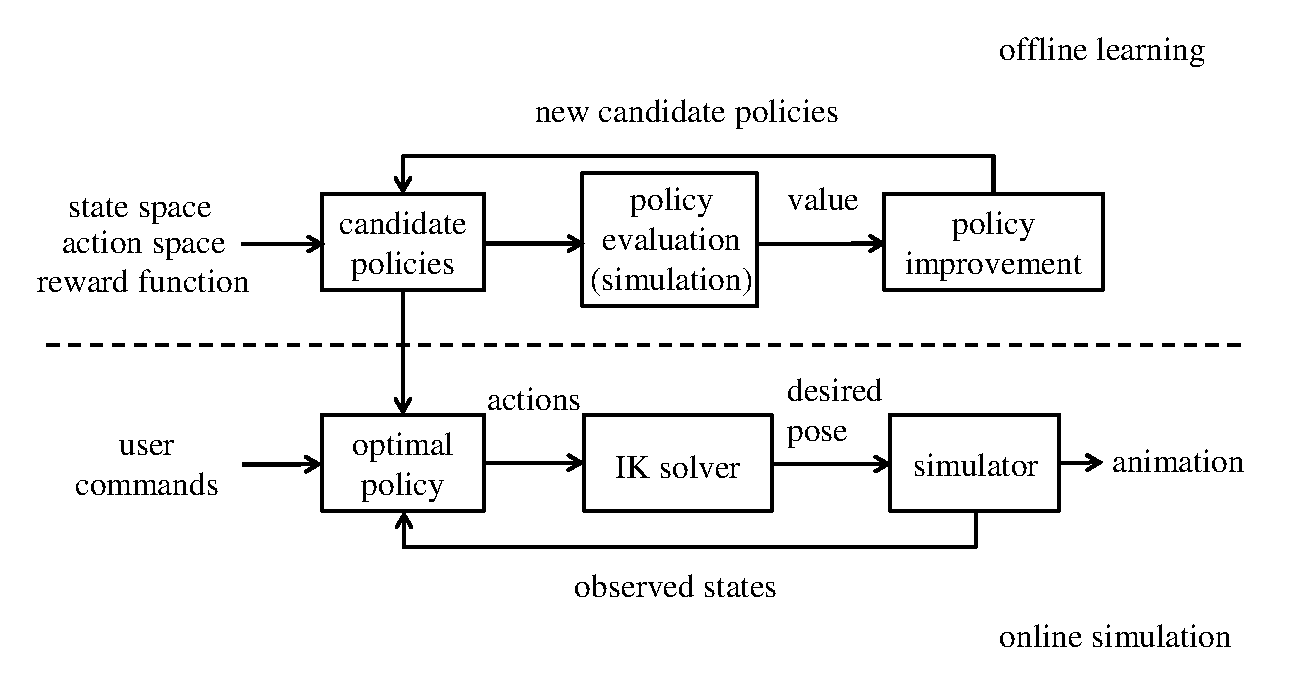
\includegraphics[width=3.4in]{figures/overview}
  \caption{Overview of our algorithm.}
  \label{fig:overview}
\end{figure}

We have designed a system that allows a virtual human character to learn to ride a bicycle and perform a wide variety of stunts. The goal of our system is to learn a control policy that initiates a particular action at any state. Given the state space, the action space and the reward function for each bicycle task, the offline learning subsystem starts with an initial set of candidate policies, iteratively evaluates (using simulation) and evolves them (using CMA or NEAT) until the optimal policy is found. This optimal policy allows the user to interact with the bicycle simulation in real time by giving commands such as steering to the left. The online simulation subsystem first extracts the observable states, such as the tilt angle, the falling speed, and the actual and the user-specified handlebar angle. It then queries the policy to determine appropriate actions, such as turning the handlebar at a certain speed to fulfill the user's command while still maintain the balance of the bicycle. Executing actions, such as turning the handlebar, requires a coordinated full-body motion of the rider. An Inverse Kinematics (IK) solver maps the compact set of actions to the rider's full-body pose. The simulator tracks this desired pose and at the same time simulates the dynamics of both the human rider and the bicycle. Figure \ref{fig:overview} illustrates the main components of our system.

\section{Bicycle and Rider Simulation}
Our simulator is based on Open Dynamic Engine (ODE) \cite{ode:2008},
but we augmented it with additional constraints to simulate both the
bicycle and the human rider. We treat the bicycle and the rider as a
system of articulated rigid bodies. Since the dynamics is represented
in the maximal coordinates, each rigid body has six DOFs and its
dynamic equation is
\begin{equation}
\left[\begin{array}{cc}
\vc{M} & \vc{0} \\
\vc{0} & \vc{I}
\end{array}\right]
\left[\begin{array}{c}
\dot{\vc{v}} \\
\dot{\vc{\omega}}
\end{array}\right]=
\left[\begin{array}{c}
m\vc{g} \\
-\dot{\vc{I}}\vc{\omega}
\end{array}\right]
+\vc{J}^T
\left[\begin{array}{c}
\vc{f}\\
\vc{\tau}
\end{array}\right]
\label{eq:dynamics}
\end{equation}
where $\vc{M}$ is the mass matrix, $\vc{I}$ is the inertia tensor, $\vc{v}$ and $\vc{\omega}$ are the linear and angular velocities, $\vc{f}$ and $\vc{\tau}$ are the constraint forces and torques, which come from the bicycle chains, the joints, the actuators and the contacts. $\vc{J}^T$ is the transposed Jacobian matrix that maps the constraint forces and torques to the body.

Chains transfer power from the pedals to the rear wheel on a bicycle. We use a linear equality constraint to realize the effect of a bicycle chain.
\begin{equation}
\vc{n}^T(\alpha\vc{\omega}_A-\vc{\omega}_B)=0
\label{eq:chainConstraint}
\end{equation}
where bodies $A$ and $B$ are the pedals and the rear wheel. $\vc{n}$ is the common direction of their rotational axes and $\alpha$ represents the gear ratio, which is the ratio between the number of teeth on the chain-ring and the number on the rear sprocket. Note that Equation~(\ref{eq:chainConstraint}) models a fixed-gear bicycle. In some tasks, we disabled this constraint to mimic the effect of the free wheel, allowing the rider to glide without pedaling.

The other constraints are standard from the implementation of ODE. For completeness of presentation, we include a brief description of such constraints in the supplementary material. Note that we use the actuator constraints instead of the traditional PD servos to track a desired pose. We have found that using the actuator constraints enables us to simulate at large time steps (0.01s), which significantly speeds up the computation.

We made several simplifications in the simulation. We used ball joints to attach the rider's feet to the pedals. This treatment is similar to wearing toe clips in the real world. We also used ball joints to connect the rider's hands with the handlebar. For some tasks in which the rider is seated, we further constrained the relative position and orientation between the rider's pelvis and the bicycle seat.


\section{Learning to Ride a Bicycle}
\label{sec:control}

\subsection{Markov Decision Process}
We formulate the bicycle control problem as a POMDP. A Markov decision process (MDP) is a tuple $(S, A, R, D, P_{sas'}, \gamma)$, where $S$ is the \emph{state} space; $A$ is the \emph{action} space; $R$ is the \emph{reward function}; $D$ is the distribution of the initial state $s_0$; $P_{sas'}$ is the transition probability; and $\gamma \in [0, 1]$ is the discount factor. For example, in the bicycle balance task, we choose the state space $S$ to include the tilt angle of the bike, the tilting speed and the handlebar angle. We choose the action $A$ to be turning the handlebar at a certain speed. We choose the reward function $R$ at the state $s$ to be
\begin{equation}
\begin{array}{ll}
R(s) = & \left\{ \begin{array}{ll}
1 & \textrm{if the bicycle remains upright,}\\
0 & \textrm{otherwise.}
\end{array} \right. \\
\end{array}
\label{eq:balanceReward}
\end{equation}
The initial state $s_0$ is drawn from a random perturbation near the upright orientation of the bicycle. The state transition is calculated using simulation, and we do not discount the rewards ($\gamma = 1$).

A \emph{policy} is a mapping from states to actions: $\pi : S \mapsto A$. The \emph{return} of a policy is the accumulated rewards along the state trajectory starting at $s_0$ by following the policy $\pi$ for $N$ steps.
\begin{displaymath}
V^\pi(s_0)=\sum_{i=0}^N{R(s_i)}
\end{displaymath}
The \emph{value} of a policy is the expected return with respect to the random initial state $s_0$ drawn from D.
\begin{equation}
V(\pi)=E_{s_0\sim D}[V^\pi(s_0)]
\label{eq:policyValue}
\end{equation}
The optimal solution of an MDP is the policy that has the maximum value $\pi^*=\arg\max_\pi V(\pi)$. The optimal policy in the bicycle balance example decides how to turn the handlebar under different situations so that the bicycle can stay upright for the longest time.

Our MDP is partially observable because we choose to observe only a selected subset of all the simulation states. We have found that focusing on a small number of relevant states for each task results in a more efficient learning process. The actions are also selected based on our prior knowledge of the task. Table~\ref{table:states} and~\ref{table:actions} summarize all the states and actions used across our different examples. The 25 states in Table~\ref{table:states} may seem exhaustive, but we only use a subset of them (typically not more than eight states) for each task.

\begin{table}[!t]
\centering
\begin{tabular}{|l|l|}
\hline
state & description \\
\hline
$t$    & time (used in the feed-forward controllers)\\
$\theta$ & handlebar angle \\
$\alpha$    & roll angle of the bike (tilt left/right)   \\
$\dot{\alpha}$     & roll speed  \\
$\beta$     & pitch angle of the bike  \\
$\dot{\beta}$     & pitch speed  \\
$\gamma$     & yaw angle of the bike \\
$\dot{\gamma}$ & yaw speed \\
$v_r$ & rear wheel linear speed \\
$v_f$    & front wheel linear speed  \\
$h_r$     & rear tire height above the ground  \\
$h_f$     & front tire height above the ground  \\
$x$    & pelvis position along x-axis\\
$y$    & pelvis position along y-axis\\
$z$    & pelvis position along z-axis\\
$\phi$    & torso orientation in the Sagittal plane\\
$\psi$    & torso orientation in the Coronal plane\\
$\chi$   & torso orientation in the Transverse plane\\
$\dot{\phi}$    & torso angular speed in the Sagittal plane\\
$\dot{\psi}$    & torso angular speed in the Coronal plane \\
$\dot{\chi}$   & torso angular speed in the Transverse plane\\
$\Delta\theta $ & difference between actual and desired handlebar angle \\
$\Delta\beta$    & difference between actual and desired pitch angle\\
$\Delta v_r $ & difference between actual and desired rear wheel speed \\
$\Delta v_f $ & difference between actual and desired front wheel speed \\
\hline
 \end{tabular}
 \caption{States and their descriptions. The rider's pelvis position, torso orientation and angular velocity are calculated in the bicycle frame's coordinates.}
 \vspace{-0.1in}
 \label{table:states}
 \end{table}

\begin{table}[!t]
  \centering
\begin{tabular}{|l|l|}
\hline
action & description \\
\hline
$\dot{\theta}$ & steering\\
$\dot{v}_r $ & accelerating or braking\\
$\dot{v}_f $ & accelerating or braking on a front-wheel-driven bicycle\\
$\tau_f$    & front braking   \\
$\dot{x}$     & pelvis motion along x-axis\\
$\dot{y}$     & pelvis motion along y-axis\\
$\dot{z}$     & pelvis motion along z-axis\\
$\dot{\phi}$    & torso motion in the Sagittal plane\\
$\dot{\psi}$    & torso motion in the Coronal plane \\
$\dot{\chi}$   & torso motion in the Transverse plane\\
$\tilde{x}$     & desired pelvis position along x-axis\\
$\tilde{y}$     & desired pelvis position along y-axis\\
$\tilde{z}$     & desired pelvis position along z-axis\\
$\tilde{\phi}$    & desired torso orientation in the Sagittal plane\\
\hline
\end{tabular}
\caption{Actions and their descriptions. The rider's pelvis and torso movements are relative to the bicycle frame's coordinates.}
\vspace{-0.1in}
\label{table:actions}
\end{table}


\subsection{Policy Search}
We apply policy search to optimize the control policies. Unlike value iteration, policy search can be easily applied to MDPs in high dimension and with continuous state and action spaces. This algorithm searches for the optimal policy within a parameterized functional space $\pi^*\in\Pi$. During policy search, one or more random policies are generated as an initial guess. These candidates are evaluated and improved iteratively. Policy improvement can be guided using the policy gradient \cite{Ng:2000:PPS}, trajectory optimization \cite{Levine2013} or other optimization techniques \cite{Heidrich-Meisner:2008}. Policy search ends when the iteration converges or the maximum number of iterations is reached.

\begin{figure*}[!t]
\centering
\includegraphics[width=\textwidth]{figures/maneuver}
\caption{A character steers the road bike towards the green arrow.}
\label{fig:balance}
\end{figure*}

\begin{figure*}[!t]
\centering
\includegraphics[width=\textwidth]{figures/staircase}
\caption{A character rides down a set of stairs without falling over.}
\vspace{-0.1in}
\label{fig:stair}
\end{figure*}

\subsubsection{Policy Parametrization}
\label{sec:parametrization}

\begin{figure}[!t]
  \centering
  \includegraphics[width=3.4in]{figures/simpleNetwork}
  \caption{Left: A simple neural network with input and output layers that are directly connected. Right: A neural network learned using our algorithm for balancing on the front wheel. Blue arrows mean negative weights while red mean positive weights. The width of the arrows encodes the magnitude of the weights. }
  \vspace{-0.1in}
  \label{fig:simpleNetwork}
\end{figure}

We use two types of parametrizations for the bicycle control problem: splines for feed-forward control and neural networks for feedback control. We found that most of the stunts can be categorized into momentum-driven, balance-driven or a combination of the two. The momentum-driven stunts involve vigorous full body motions to manipulate the bicycle to a desired orientation. Coordinated full body motions with large magnitude are essential, but the short duration of this type of stunts makes balance easy to maintain. For this reason, we use feed-forward controllers and represent the action trajectories as cubic Hermite splines. Assuming that the number of control points is given, the parameters to optimize are the time and the value of the control points\footnote{We do not optimize the tangents at the control points and we set them to be zero.}.

Balance-driven stunts require that the rider carefully adjusts his or her COM and maintains a stunt pose for a longer period of time. Feedback balance control is vital to the duration of the performance, which determines the success or failure of the stunt. We use neural networks for their ability to approximate a wide range of functions. The inputs to a network are the observed states, and the outputs are the actions. Figure~\ref{fig:simpleNetwork} Left illustrates a simple neural network that directly connects the input and the output layers. The output of neuron $i$ is
\begin{displaymath}
v_i=\sigma(\sum_j w_{ij} v_j)
\end{displaymath}
where $w_{ij}$ is the connection weight between neuron $i$ and $j$, and $\sigma$ is the sigmoid function $\sigma(x) = 1/(1+e^{-x})$.

Parametrization determines the potential quality of the optimal policy. The network shown in Figure~\ref{fig:simpleNetwork} Left is too simple for representing a complex policy required by bicycle stunts. However, it is not clear how to manually design the network structure, given the control policies of unsuccessful stunts. For this reason, we use NEAT to search for both the structure of the neural network and its weights simultaneously, which finds far better policies than searching over a fixed network. Figure~\ref{fig:simpleNetwork} Right demonstrates the learned network for the balance task of a bicycle endo using NEAT. See Section~\ref{sec:improvement} for more details.

\subsubsection{Policy Evaluation}
To evaluate a policy, we formulate a reward function in the following form:
\begin{equation}
R(s)=R_t(s)+wR_r(s)
\end{equation}
where $R_t$ and $R_r$ are task-specific and regularization terms respectively. $w$ is the weight.

We use eq.(\ref{eq:balanceReward}) as the task-specific reward for balance-driven tasks. As the reward is accumulated over time, the return counts the number of frames that the bicycle stays upright. The task-specific reward varies for each momentum-driven stunt. For example, the reward for initiating an endo (lifting the rear wheel) is to maximize the negative pitch angle of the bike $R_t=-\beta$. We refer the readers to Section \ref{sec:results} and for more detailed descriptions of task-specific rewards.

Given the task-specific reward term alone, multiple optimal policies could exist. Taking the balance task as an example, a policy that rides in a straight line and another that oscillates in a sinusoidal path by periodically swinging the handlebar can both balance well and thus yield the same value. The regularization term is mainly used to eliminate this ambiguity. We use the regularization term $R_r=\frac{1}{|\theta|+\epsilon}$ to express our preference of riding straight. In our examples, all the regularizers are in the form of
\begin{displaymath}
R_r = \frac{1}{|X|+\epsilon}
\end{displaymath}
where $X$ can be substituted by $\alpha$ for the upright bicycle position, $\Delta \theta$ for the desired steering angle, $\Delta \beta$ for the desired pitch angle, $\Delta v$ for the desired speed, $(x, y, z)$ and $(\phi, \psi, \chi)$ for small changes of rider's pelvis position and torso orientation. A small number $\epsilon$ in the denominator is used to bound the reward.

We do not explicitly minimize the rider's effort in the reward function because it is difficult to balance the effort minimization objective and the task-specific objective for difficult stunt actions. However, we limit the maximum actuated joint torques of the rider in the simulation to ensure that the rider does not possess super-human strength.

We run multiple simulations with different initial configurations $s_0$, which are sampled from random perturbations of the default bicycle velocity and orientation, to evaluate the value of a policy. At each simulation step, our algorithm calculates the reward for the current state, and accumulates this until the bicycle falls or after 1000 time steps. The average return of all the simulations is the value of the policy.

\begin{figure*}[!t]
\centering
\includegraphics[width=\textwidth]{figures/Curb}
\caption{A character lifts the front wheel to ride over a curb.}
\label{fig:curb}
\end{figure*}

\begin{figure*}[!t]
\centering
\includegraphics[width=\textwidth]{figures/endo}
\caption{A character performs an endo and balance on the front wheel.}
\vspace{-0.1in}
\label{fig:endo}
\end{figure*}

\subsubsection{Policy Improvement}
\label{sec:improvement}

Many policy improvement methods utilize the policy gradient \cite{Peters:2008} to perform iterative ascending operations. However, our simulation of bicycle stunts involves frequent discrete events such as establishing and breaking contact, which invalidates the gradient information. For this reason, we use sample-based stochastic optimization techniques. We apply CMA to search for the feed-forward controllers since the parametrization of splines is fixed. We use NEAT to search for feedback controllers, including the structure and the weights of the neural network. NEAT has many similarities to genetic algorithms, but it is tailored to the creation of neural networks. We will describe NEAT briefly below. For further details we refer readers to the original paper \cite{Stanley:2002:ENN}.

NEAT iteratively performs evaluation, selection, crossover and mutation. To maximize the value of a policy, NEAT starts with a simple network structure, in which the input and the output layers are directly connected. A population of such networks with random weights is drawn as an initial guess. These candidate policies are evaluated and the top 20\% are selected to survive. Pairs of randomly-selected surviving policies are crossed over to produce a new generation (more on this below). Mutations (with low probability) can perturb connection weights, add a neuron or add a connection. Note that the addition of a neuron or a connection complexifies the network structure and enriches the class of functions that it can represent.

Crossover is nontrivial in NEAT because the parent neural networks can have different topologies. To overcome this difficulty, the newly-added neuron or connection is assigned a unique innovation number, which tells the history of the mutation and how to match up neurons or connections between parents during crossover. The neurons or connections that share the same innovation number across parents are from the same ancestor, which will be inherited randomly by the child sample. The neurons or connections that have no counterparts in the other parent are from different mutations. They will be inherited from the parent with the higher value.

The evolution ends when the policy values do not increase over a certain number of iterations or the maximum number of iterations is reached.

\section{Results}
\label{sec:results}

\begin{figure*}[ht]
\centering
\includegraphics[width=\textwidth]{figures/frontWheelPivot}
\caption{A character completes a quick 180-degree turn by pivoting the bicycle on the front wheel.}
\label{fig:pivot}
\end{figure*}


\begin{figure*}[ht]
\centering
\includegraphics[width=\textwidth]{figures/bunnyHop}
\caption{A character performs the American bunny hop over a clown lying on the ground.}
\vspace{-0.1in}
\label{fig:bunnyhop}
\end{figure*}

\begin{figure*}[ht]
\centering
\includegraphics[width=\textwidth]{figures/velocipede}
\caption{A character rides a high wheeler and performs a stunt in which he rides backward on a single wheel.}
\label{fig:highwheeler}
\end{figure*}

\begin{figure*}[ht]
\centering
\includegraphics[width=\textwidth]{figures/unicycle}
\caption{A clown rides a unicycle.}
\vspace{-0.1in}
\label{fig:unicycle}
\end{figure*}

In this section we describe the results of our system. Please watch the accompanying video for the bicycle riding and stunt
animations. Our system was implemented in C++, and we used ODE with additional chain constraints to simulate both the bicycle and the human rider. The simulator runs in real time on a desktop workstation with a 2.26GHz CPU and 4GB of memory. We generated 90 samples per iteration and 50 iterations for offline policy search. The computations were distributed across 16 CPU cores on a cluster. The learning time ranges from a few minutes to half an hour depending on the number of simulations used to estimate the expected return (eq.~\ref{eq:policyValue}). Table~\ref{table:stateActions} summarizes the choices of states and actions for each bicycle task.

We designed three different bicycles and a unicycle to test our controllers on a variety of tasks. \emph{Road bikes} (Figure~\ref{fig:balance}) are designed to travel at speed on paved roads. They have very narrow tires to reduce the rolling resistance. The seats are mounted high so that the riders can bend their upper bodies down for less air resistance. We use a \emph{BMX bike} (Figure~\ref{fig:endo}) for stunts. BMX bikes are usually considerably smaller for nimble and agile handling. They have fat tires to facilitate balance and to increase traction. BMX bicycle parts can often be customized to meet the needs of different stunts. \emph{High wheelers} (Figure~\ref{fig:highwheeler}) are an old style of bicycle appearing in the late 19th century. They have a large front wheel and a much smaller rear wheel. This peculiar design makes high wheelers difficult to ride due to the center of mass being high and not far behind the front wheel. Any sudden stop could send the rider over the handlebars. A \emph{unicycle} (Figure~\ref{fig:unicycle}) has only one wheel and no handlebar. The rider needs to be concerned about the balance in both the longitudinal and the lateral directions. Different cycle designs greatly affect the handling characteristics and change the behavior of the riders. This variety puts the generality of our algorithm to the test. We modeled all the cycles and calculated their mass properties in SolidWorks.

\begin{table}[!b]
\vspace{-0.1in}
\centering
\begin{tabular}{|l|c|c|}
\hline
task & states & actions \\
\hline
momentum-driven & & \\
\hline
going over curbs      & $t, \beta$   & $\dot{v}_r, \tilde{\phi}$\\
endo (lifting)        & $t, \beta$  & $\tau_f, \tilde{y}, \tilde{z}$ \\
front wheel pivot     & $t, \dot{\gamma}$ & $\dot{\theta}, \tau_f, \tilde{y}, \tilde{z}$\\
bunny hop             & $t, h_f, h_r$ & $\tilde{y}, \tilde{z}$\\
\hline
balance-driven & & \\
\hline
balance and steering  & $\theta, \Delta \theta, \alpha, \dot{\alpha}$ & $\dot{\theta}$ \\
wheelie               & $\alpha, \dot{\alpha}, \beta, \dot{\beta}, \Delta \beta, v_r, \psi, \dot{\psi}$  & $\dot{v}_r, \dot{\psi}$ \\
endo (balance)        & $\theta, \alpha, \dot{\alpha}, \beta, \dot{\beta}, \Delta \beta$ & $\dot{\theta}, \tau_f$ \\
back hop              & $\alpha, \dot{\alpha}, \beta, \dot{\beta}, \Delta \beta, x, y, z$ & $\dot{x}, \dot{y}, \dot{z}$\\
high wheeler (stunt)  & $\beta, \dot{\beta}, \Delta \beta, \Delta v_f$ & $\dot{v}_f$\\
unicycle              & $\alpha, \dot{\alpha}, \beta, \dot{\beta}, v_r, \Delta v_r, \chi$ & $\dot{v}_r, \dot{\chi}$\\
\hline
 \end{tabular}
 \caption{Choices of states and actions for each bicycle task. Note that in the momentum-driven tasks, the actions only depend on time $t$ while the remaining states are used to compute the reward. }
 \label{table:stateActions}
 \end{table}

\paragraph{Balance and steering.} Riding a bicycle requires balance and steering. Balance can be maintained by steering toward the falling direction, which generates centrifugal force to push the bike upright. Figure~\ref{fig:balance} shows that our learned controller enables the rider to balance and steer the bike towards a user-specified direction. The bike follows the green arrow closely even when the user changes the desired direction abruptly. This agile steering behavior is achieved through ``counter-steering'': a momentarily steering in the opposition direction to initiate a sharp turn~\cite{Rankine1870}, which emerged automatically from the policy search. We also tested the robustness of our balance and steering controller on a bumpy terrain, which is represented as a noisy height field sampled from a uniform distribution $h\sim U(0, 0.05)$ (unit: meter). Even though the bicycle jumps and the handlebar is perturbed constantly, the rider still manages to balance and closely follows the desired direction. In addition, the accompanying video shows an initial starting motion, in which the rider's left foot is scripted to push the ground and move towards the pedal. Based on this single trajectory of foot and the learned balance policy, we used IK to generate the full-body motion of the starting phase.

\paragraph{Going down stairs.} Figure~\ref{fig:stair} shows the character riding down a series of stairs. Each step is 0.15m high and 0.8m wide. We used the same balance controller as in the previous example. This balance task is more challenging because the frequent loss of contact and the sudden collisions between the front tire and the ground narrow the window of effective control and introduce large perturbations. Initially, the rider needs to make large corrections with the handlebar to keep balance when the forward speed is low. As the bicycle travels faster, the corrections become smaller and steadier.
\vspace{-0.05in}

\paragraph{Going over curbs.} Riding over curbs (Figure~\ref{fig:curb}) can be performed by lifting the front wheel using feed-forward control only. We therefore parameterized the actions with two splines (Table~\ref{table:stateActions}) and trained the controller using CMA. We used a task-specific reward function to maximize the pitch of the bicycle $R_t = \beta$ during lifting. In the animation, as the bicycle approaches a curb (0.12m high), the rider first leans forward and then pushes her upper body backwards. When the arms are stretched out to the maximum length, the sudden deceleration of the upper body pitches the whole bike upwards. The pitch angle is further increased by pedaling faster. This sequence of highly coordinated movements is discovered automatically by the policy search algorithm. Once the front wheel goes over the curb, the balance controller takes over and keeps the bike upright when the rear wheel hits the curb.
\vspace{-0.05in}

\paragraph{Real time user interaction.} A user can interact with our bike simulation in real time. We video captured a sequence that shows a person using a joystick that is equipped with motion sensors to control the rider and the bicycle. The rider goes over a curb, survives a crosswind, goes down a set of stairs, and follows a curvy path to the goal. Note that the user only gives high level commands such as the desired steering angle and the timing of lifting the front wheel. The balance, the actual steering and the rider's motions are all controlled by the policy learned from the offline training process.
\vspace{-0.05in}

\paragraph{Wheelie.} A wheelie is a stunt maneuver in which the rider first lifts the front wheel and maintains balance on only the rear wheel. Lifting the front wheel on a BMX bike is considerably easier than on a road bike due to the shorter distance between the wheels. It can be achieved by increasing the speed of pedaling without any noticeable upper body movements. For this reason, we used only a feedback controller (Table~\ref{table:stateActions}) to perform a wheelie, including both the initial lift and the later balance. Once the front wheel leaves the ground, the rider adjusts the forward speed to keep the desired pitch angle. He leans his upper body to the left or to the right to correct any lateral instability.
\vspace{-0.05in}

\paragraph{Endo.} Figure~\ref{fig:endo} shows an endo. In contrast to a wheelie, an endo lifts the rear wheel and balances on the front wheel. In spite of its symmetry to a wheelie, an endo requires an entirely different set of skills and environments. Endos are usually performed on a gentle downward slope, which provides the needed forward momentum when the driving wheel is off the ground. We used a slope of 2.5 degrees in our example. We first search for a feed-forward controller that maximizes the negative pitch angle $R_t = -\beta$ to initiate the stunt. The resulting controller slowly moves the rider's pelvis to the back, and then quickly throws it to the front to lift the rear wheel.

The feed-forward controller is succeeded by a feedback balance controller. To maintain an endo, the rider continuously applies or releases the front brake for longitudinal balance and steers the handlebar towards the direction of leaning for lateral balance. This stunt is especially challenging. If the pitch angle is too large, when the COM is above or in front of the front tire contact, such a gentle slope cannot provide enough acceleration to prevent overturning. If the pitch angle is too shallow, to prevent the rear wheel from dropping to the ground, braking hard will quickly halt the bicycle and make the balance strategy of ``steering toward falling'' ineffective. This complicated coupling between the pitch angle, the speed and the lateral balance makes heavy demands on the policy search algorithm. NEAT successfully finds a policy that can maintain balance for an extensively long period of time. Figure~\ref{fig:simpleNetwork} Right illustrates the complex neural network required for this task.

In the accompanying video, we also demonstrate the learning process of an endo. The animation shows the resulting balance controller after one, five and ten iterations. As more iterations are finished, the rider gradually masters an endo and maintains balance for a longer period of time.

\paragraph{Front wheel pivot.} A front wheel pivot (Figure~\ref{fig:pivot}) is a fast way to turn the bicycle 180 degrees by pivoting on the front wheel. We used a feed-forward controller and applied two separate task-specific rewards during two phases of this motion. The first reward function maximizes the angle of turning during the pivoting phase.
\begin {displaymath}
\begin{array}{ll}
R_{t_1} = & \left\{ \begin{array}{ll}
\dot{\gamma} \Delta t & \textrm{if }h_r > 0.01,\\
0 & \textrm{otherwise.}
\end{array} \right. \\
\end{array}
\end {displaymath}
After the rear wheel touches the ground, we switch to a learned balance controller and measure how long the bicycle can stay balanced: $R_{t_2}=1$ if the bicycle remains upright. Without the second reward function, the ``optimal'' policy can produce a large roll during the pivoting phase, after which the rider cannot recover balance. In the animation, the rider performs an endo after turning the handlebar sharply to the left. As a result, the rider and the bike pivot around the front wheel and the 180-degree turn finishes within three seconds.
\vspace{-0.05in}

\paragraph {Back hop.} The back hop is another way to balance on the rear wheel. This feedback balance strategy uses small hops to change the relative position between the contact and the COM. In the animation, the rider and the bike start at an initial pose in which the COM is behind the contact point between the rear wheel and the ground. The bike will fall backwards if the rider does not correct for this. He bends his knees and then extends them to bring the rear wheel off the ground. He quickly pulls the handlebar towards himself in mid-air to adjust the pitch of the bicycle. When the rear wheel lands, the COM comes closer to the ground contact position. As a result, the rider can continue to hop and balance for a long time.
\vspace{-0.05in}

\paragraph{Bunny hop.} Figure~\ref{fig:bunnyhop} shows the rider performing a bunny hop on a BMX bike. A bunny hop is a stunt where the rider jumps with the bike over an obstacle or a trench. The task-specific reward function for the feed-forward controller is evaluated based on the height of both tires above the ground $R_t=h_fh_r$. Right before the hop, the rider first leans forward and then moves his pelvis rapidly towards the back of the bicycle. This vigorous motion tilts the bicycle upward. The rider then jumps with the bicycle over a clown lying on the ground. We were pleased to see that the optimal policy for the bunny hop motion includes a phase that tilts the bicycle up, which is essential to jumping for a greater height and distance. This style is known as the ``American bunny hop''.
\vspace{-0.05in}

\paragraph{Riding a high wheeler.} The peculiar design of a high wheeler makes ``headers'' a significant hazard, in which the rider gets pitch forward off the bicycle. We took on the challenge and designed a stunt that we had never seen performed on a high wheeler (Figure~\ref{fig:highwheeler}). During the stunt, the rider intentionally stops the bike to initiate a forward rotation. He then carefully changes pedaling speed to avoid taking a header and successfully rides backward on a single wheel. The rider can balance for a few seconds even without a lateral balance controller, probably due to the prominent gyroscopic effect from the large rotating front wheel. When the rider starts to lose balance, he accelerates to return to the normal riding mode, in which we used the same balance and steering controller as in the road bike examples.
\vspace{-0.05in}

\paragraph{Riding a unicycle.} The unicycle and the bicycle have many similarities. We have found that our algorithm is general enough to handle balance on a unicycle. Similar to some bicycle stunts, the longitudinal balance on a unicycle can be maintained via speeding-up or slowing-down, while the lateral balance can be maintained through steering toward falling. Unfortunately, unicycles do not have handlebars to steer. To steer the unicycle to the left, the rider needs to twist his upper body to the right. The unicycle will counter-rotate to the left due to the conservation of angular momentum. Figure~\ref{fig:unicycle} shows a clown riding a unicycle. To start riding, the clown first pedals backward, which leans the unicycle to the front. He then accelerates until the actual speed matches the user-specified desired speed. During riding, the clown repeatedly twists his waist to keep the lateral balance, which causes the unicycle to travel in a slightly sinusoidal path.



\section{Discussion and Limitations}
\label{sec:Evaluation}

\begin{table*}[ht]
\vspace{-0.1in}
\centering
\begin{tabular}{|l|c|c|c|c|c|c|c|c|c|}
\hline
task & wrist & elbow & scapula & shoulder & pelvis & hip & knee & ankle & ratio \\
\hline
\begin{tabular}{@{}l@{}}balance and \\steering (flat)\end{tabular} & 50 (5) & 150 (20) & 200 (30) & 550 (40) & 2000 (100) & 500 (150) & 500 (50) & 500 (50) & 0.9\\
\hline
unicycle & 10 (1) & 100 (5) & 100 (20) & 150 (10) & 2000 (30) & 100 (95) & 100 (90) & 60 (20) & 0.89\\
\hline
wheelie  & 10 (10) & 100 (30) & 100 (50) & 150 (80) & 2000 (100) & 500 (150) & 100 (100) & 60 (60) & 0.81\\
\hline
\begin{tabular}{@{}l@{}}going over \\curbs\end{tabular}& 50 (30) & 150 (50) & 200 (50) & 550 (80) & 2000 (100) & 500 (150) & 500 (100) & 500 (60) & 0.76\\
\hline
high wheeler & 50 (10) & 150 (50) & 200 (20) & 550 (200) & 2000 (300) & 500 (440) & 500 (360) & 500 (230) & 0.64\\
\hline
\begin{tabular}{@{}l@{}}balance and \\steering (bumpy)\end{tabular} & 50 (50) & 150 (100) & 200 (100) & 550 (350) & 2000 (400) & 500 (300) & 500 (350) & 500 (200) & 0.58\\
\hline
\begin{tabular}{@{}l@{}}front wheel \\pivot\end{tabular} & 250 (50) & 500 (150) & 500 (150) & 550 (400) & 2000 (600) & 500 (500) & 500 (280) & 500 (80) & 0.58\\
\hline
staircase & 50 (40) & 150 (100) & 200 (90) & 550 (350) & 2000 (400) & 500 (450) & 500 (450) & 500 (80) & 0.56 \\
\hline
bunny hop & 20 (15) & 50 (50) & 500 (150) & 550 (150) & 2000 (750) & 500 (400) & 500 (380) & 500 (220) & 0.44\\
\hline
endo & 50 (50) & 100 (100) & 100 (100) & 550 (400) & 2000 (600) & 500 (470) & 500 (485) & 500 (150) & 0.45\\
\hline
back hop & 250 (90) & 500 (400) & 500 (500) & 550 (545) & 2000 (900) & 500 (500) & 500 (450) & 500 (140) & 0.33\\
\hline
 \end{tabular}
 \caption{Torque limits (Unit: Nm) for different tasks. The values without the parenthesis are used for learning. The values within the parenthesis are the lowest torque limits that can be used in the simulation before the motion starts to fail. The amount of reduction is a measure of the robustness of the learned controllers. More reduction means a more robust controller. The last column reports the reduction ratios of average torque limits, which are sorted from high to low. This ranking is a possible indication of the difficulties (from low to high) that the learning algorithm think for each task. }
 \vspace{-0.1in}
 \label{table:torqueLimit}
 \end{table*}


Although the learning algorithms presented in this paper are general, the qualities of simulated motions vary with different tasks. We notice that some of the stunt motions do not look as compliant as those performed by real human riders due to three possible reasons. First, we chose large torque limits to allow robust control for various challenging maneuvers (Table~\ref{table:torqueLimit}). We used the same torque limits both in offline learning and online simulation to generate the results shown in the accompanying videos. To investigate whether we can achieve more compliant motions, we reduce the joint torque limits for simulation until the rider can no longer maintain balance (shown as the values in the parenthesis in Table~\ref{table:torqueLimit}). Although our controllers are robust when executed with smaller amount of torques, the resulting human motion appear very similar. The second possible reason is that we did not minimize rider's effort during offline learning. We found that it is difficult to weigh the effort minimization term because it competes with the task-specific objective. One possible solution is to implement prioritized optimization \cite{delasa:2009} to incorporate the effort minimization objectives. The last reason is probably due to the use of actuator constraints in ODE. The actuator constraints usually result in more stable simulation. However, since the joint torques are solved together with all other constraint forces, this allows the character to react instantaneously. We believe that the lack of reaction latency contributes to the stiffness of the motion. Using traditional PD servos could mitigate this problem but could also significantly increase the time of learning and simulation.


\begin{figure}[ht]
  \centering
  \includegraphics[width=3.4in]{figures/TorquePlot}
  \caption{Torque trajectories over time of performing an endo and riding a bicycle on a flat ground. }
  \label{fig:torquePlot}
\end{figure}

We further examine the torque trajectories (Figure~\ref{fig:torquePlot}), and observe that the controllers learned different strategies to achieve different tasks. In the endo example, the torques switch abruptly between the two extreme values. It is similar to the ``bang-bang control'' that frequently arises in time-critical tasks, indicating that the task of endo might also be time-critical. In contrast, the torque trajectory of riding a bicycle on a flat terrain shows more smooth transitions, which implies that normal biking does not require instant reactions and is thus an easier task.

\begin{figure*}[ht]
  \centering
  \includegraphics[width=\textwidth]{figures/NeatCMAComp}
  \caption{A comparison between policy searches with a fixed and an evolving parametrization. Left: The policy value vs. the number of iterations for ten policy searches on a fixed parametrization using CMA. Middle: Results of ten policy searches on a fixed parametrization using neuroevolution without augmenting topology. Right: Results of ten policy searches on an evolving parametrization using NEAT. }
  \label{fig:compare}
\end{figure*}

We have demonstrated that searching for both the parametrization and the parameters of a policy creates robust controllers for a wide variety of bicycle balance tasks. Since many previous studies focused on optimizing the parameters alone, we evaluated the necessity of optimizing the parametrization.
Figure~\ref{fig:compare} Left and Right compares two policy search results with a fixed and with an evolving parametrization for the balance task of an endo. Both searches started with the same parametrization: a neural network with direct connections between the input and the output layers. We used CMA to search for only the weights while we used NEAT to evolve both the weights and the network structure. Both algorithms were run for 50 iterations with 90 samples per iteration. We ran each search ten times with different random seeds to reduce the stochastic bias. Figure~\ref{fig:compare} Left plots the curves of the policy value versus the number of iterations in the CMA search. Note that none of the searches reached a value of 3000. In comparison, eight out of ten NEAT searches found policies scored higher than 3000 (Figure ~\ref{fig:compare} Right). Three of them reached almost 7000. The average final policy value of NEAT was almost twice its CMA counterpart. A similar comparison was conducted between neuroevolution with and without augmenting topology, and this told the same story (Figure~\ref{fig:compare} Middle vs. Right). Even though we only reported the detailed comparison for this particular example, we observed the same trend for other bicycle stunts: policy search with an evolving parametrization significantly outperforms search with a fixed parametrization. The neural network structure for all the balance-driven tasks are shown in the supplementary material.

As illustrated in Section \ref{sec:results}, many bicycle stunts need balance in both the longitudinal and lateral directions. In our implementation, we decoupled the balance task in these two directions and learned the task in two steps. In the first step, we focused on longitudinal balance and chose only the relevant states and actions. We artificially increased the width of the tire to 20cm so that the controller did not need to be concerned about the loss of balance in the lateral direction. This is analogous to using training wheels in real life. Once the longitudinal controller had been learned, we fixed that part of the neural network, reduced the width of the tire back to normal\footnote{The tire width of the road bike and the high wheeler is 1.5cm while the tire width of the BMX bike and the unicycle is 3cm.} and then performed the second step of training for lateral balance. Although in theory, optimizing a controller for the longitudinal and the lateral balance simultaneously would have a better global optimum, in practice, searching for a policy in a higher dimensional space is subject to local minima and thus could produce inferior results. In all our examples, this two-step training found better policies than training both longitudinal and lateral balance simultaneously.

Our attempts at learning bicycle stunts using other reinforcement learning algorithms ended up unsuccessful, but these valuable experiences led us to our current solution. Our first attempt was to use standard value iteration method with a discretized state space. The high dimensional state space made the tabular representation infeasible. We encountered the convergence issue when the state space was parameterized by polynomial and Gaussian kernel bases. We also experimented with a few model-free learning algorithms. For example, SARSA($\lambda$) demonstrated some potential (\ie the normal cycling was successful), but the computation time was too long even for the simplest task. Although our final decision was to use policy search, the initial experiments were unsuccessful due to an overly simplified policy parametrization: a neural network without hidden layers. Using quadratic features to enrich the inputs of the network, we had some limited success with the optimal solutions solved by CMA. However, without a systematic way to perform feature selection, the likelihood of finding a successful local minimum is low due to the large number of quadratic features. Finally, we chose NEAT, a bottom-up approach that complexifies the parametrization from the simple network. This method consistently found policies that worked for all our examples.

NEAT provides an effective way to search for both the parametrization and the parameters, which frees us from laborious and unintuitive manual tuning of the network structure. However, to formulate an MDP, we still need to design the state space, the action space and the reward function. While designing the state space is often straightforward, choosing appropriate actions for a specific task requires domain knowledge. For example, knowing how to steer a unicycle is essential for the unicycle balance task. Likewise, designing a good reward function requires some trial-and-error experiments. Our reward functions initially contained only the task-specific terms. We found that the algorithm often discovered a policy that had a high value but resulted in undesired motions: The rider performed redundant movements as long as this did not affect the balance. We eliminated these undesired motions by adding regularization terms to the reward function. However, selecting states, actions and reward functions is unavoidable when formulating and solving MDPs. Inverse reinforcement learning \cite{Ng:2000} might be a promising approach, but this requires data generated from the optimal policy, such as motion capture data from real stunt bikers. Compared to manually designing a policy parametrization, learning the domain knowledge and tuning the reward function is more intuitive and fun.

Our system has a few limitations. We used ball joints to attach the feet to the pedals. These bilateral joint constraints simplify the simulation but render some motions less realistic: The brief moment in our bunny hop animation when the rear wheel pops off the ground just before the hop typically is not seen in the real stunt. Faithfully modeling the contact between the feet and the pedals could solve this problem. However, this will make the simulation more expensive and the learning more difficult. In the learning, we separated the feed-forward and feedback controllers. This treatment works well if the feed-forward controller is applied for a short period and then we switch to the feedback controller. However, in a real-life performance, stunt bikers exhibit both feed-forward and feedback controls at the same time, which allows them to perform longer and more difficult stunts. This might be one of the reasons that our algorithm cannot generate a 360-degree front wheel pivot. Our interactive simulation does not allow the user to arbitrarily concatenate the stunts. Successful stunts demand a stable initial pose, appropriate speed and sometimes a favorable terrain. All these requirements together prevents us from concatenating stunt controllers arbitrarily. Learning additional intermediate controllers between stunts might be a possible solution.

\section{Conclusion}

We have presented an algorithm for animating bicycle stunts.  Key aspects of our approach include a fast and stable physical simulation,
policy search for POMDP, and
the use of a sample-based optimization solver that searches for both the structure and the weights of a neural network.
Our system allows us to control a human character that
performs a variety of bicycle stunts, including wheelie, endo, bunny hop, front wheel pivot and back hop.
Our characters can learn to master the most demanding balance tasks in minutes, which challenges most people and takes months of practice to learn.

Policy search is a powerful method for learning optimal controllers. However, manually designing parametrization of the policies could be challenging for difficult tasks. Combining policy search with NEAT makes it easy to use and unleashes its full power. We believe that its success will not be limited to the bicycle control tasks. It has the potential to solve other challenging control problems, such as gymnastics, skateboarding, surfing and dancing.

There are a number of interesting avenues for future work. Deep learning \cite{Hinton:2007} and deeper neural networks could be explored for even more difficult stunts. Our work has concentrated on controllers for individual stunts. It would be interesting to investigate a sequence of stunts that traverse a bicycle course with obstacles. Finally, it would be fascinating to manufacture a mini bicycle and a robotic rider and apply our controllers to make them perform stunts in the real world.

\chapter{Locomotion Controller Transfer from Virtual To Real World}
\section{Motivation}
Robotics and character animation share a common goal, to design locomotion controllers, the algorithmic ``brain'' that allow animated characters and robots to move naturally, robustly and efficiently in a complex dynamic environment. Despite this commonality, there is a gap between the state-of-the-art of these two fields. While in character animation, we have demonstrated that it is possible to control a full humanoid character to perform challenging locomotion tasks in a physically simulated environment, we have not yet seen any robots that have comparable capabilities. For example, controlling human walking is considered as a solved problem in character animation, but it is still an open research in robotics. In addition, we have demonstrated in the previous Chapters that with the powerful computational tools, controller can be optimized autonomously in a virtual environment. However, in robotics, designing controllers is still a challenging, trial-and-error process that is limited only to highly-specialized engineers. Can we extend the computational tools developed for character animations to robotics to close the gap between these two fields?

One major challenge to directly applying the methods we have developed to control robots is the Reality Gap: Controllers that work effectively for a virtual character in the simulation may perform poorly on a robot in the real environment. The most important factors that lead to the Reality Gap include hardware limitation, unmodelled dynamics, inaccurate physical properties, noise and latency. For example, the torque limits of the servos on the robot are seldom considered in animation applications. We also do not model the dynamics of the servos. Even though we often can acquire the physical properties, such as mass, center of mass and inertia, of a robot from its CAD files, they are usually inaccurate given the manufacturing error, assembly error and the cables that are not considered in CAD files. Furthermore, the noise in the environment and the latency in hardware communication also contribute to the Reality Gap.

To cross the Reality Gap and to design robotic controllers autonomously, we develop a system with three components, physical simulation, controller optimization and simulation calibration. We first build a physical simulation of articulated rigid bodies to model the dynamics of the robot and its environment. Different from the simulators used in animation, we incorporate the torque limits, servo dynamics, noise and latency measured from the robot experiments into our simulator. We then optimize a controller for a specific locomotion task in the physical simulation. However, if we apply this optimal controller directly to the robot, it will fail the task in the real world due to the Reality Gap. To solve this problem, we collect the real performance data, and use it to calibrate our physical simulator. We optimize a set of simulation parameters, including the mass, inertia, center of mass and actuator gains of the robot, to minimize the discrepancy between the simulation results and the collected real data. Through calibration, the simulator can capture the real world dynamics more faithfully. This calibrated simulator is used again in controller optimization to improve the quality of the controller. Depending on the task, it could take several iterations of simulation calibration and controller optimization to transfer the controller to the real robot. 

We evaluate our system in three locomotion tasks, rising from a leaning, sitting, or kneeling position to an erect stance. These motions are widely used in our daily life. Although most of us can perform them with ease, it is a big challenge for some elderly persons and patients with hamspring injuries. We choose to study these motions and synthesize them on robots due to these important health-care applications. One simple solution to achieve these tasks is to use static balance. The robot increases the area of the contact polygon by establishing more contact points, and then rises its body slowly while maintaining the COM within the contact polygon. We choose not to use this strategy because in real life, we human can perform these motions in a more agile fashion, and we hope that our controller can enable robots to demonstrate comparable agility. For this reason, our controllers will utilize impulsive actions and take advantage of the dynamic motion to rise. In addition, since one main contribution of our method is simulation calibration, to best test its effectiveness, we only use feedforward controllers in our evaluations. In contrast, if feedback controllers are used, the stability region of the task would be drastically increased, which makes the simulation accuracy less critical. Our results show that simulation calibration is effective. In most cases, only one iteration of calibration is needed to transfer the controller successfully to the real robot. Our system is able to design locomotion controllers autonomously, which work successfully both in the simulation and in the real world. 

\section{Overview}

\begin{figure}[!t]
  \centering
  \includegraphics[width=6in]{figures/controllerTransfer}
  \caption{Overview of our algorithm.}
  \label{fig:controllerTransferOverview}
\end{figure}

We have designed a system that can automatically design locomotion controllers for robots (Figure~\ref{fig:controllerTransferOverview}). Given the specification of the robot, including its body shape, the physical properties of each body, and the types of joints, we build a physical simulation using Dynamic Animation and Robotics Toolkit (DART) \cite{dart:2012}, an open source articulated rigid body simulator. In addition, we also take into consideration the torque limits, servo gains, noise and latency, which are not modeled in DART. The controller optimization subsystem runs thousands of simulations to search for the optimal controller to minimize the task-related objective function. We then test this optimal controller on the robot. If the robot successfully completes the task, a working robotic controller is found and our algorithm terminates. Otherwise, we record the robot performance data and feed it into the simulation calibration subsystem. Simulation calibration runs another optimization, which searches for the optimal simulation parameters to minimize the discrepancy between the performance data from the simulation and that from the robot experiments. The loop of controller optimization and simulation calibration is performed iteratively until the controller works successfully on the real robot. In the next three sections, we will delve into the details of these main components of our system, physical simulation, controller optimization and system calibration.

\section{Physical Simulation}
\section{Controller Optimization}
\section{System Calibration}
\section{Results}
\section{Discussion}

\chapter{Conclusion and Future Work}

\section{Conclusion}
In this dissertation, we have presented a principled way to synthesize locomotion of humans and animals. Our algorithms can control characters of different morphologies to move efficiently and robustly in complex physically-simulated environments and to achieve challenging tasks. The key components of our algorithms are a set of powerful computational tools, including physical simulation and controller optimization. Although combining simulation and optimization is not a novel idea in motion synthesis, in contrast to prior work, we examine and identify those commonly-used simplifications that can affect the quality of the motions. We eliminate these simplifications by designing new simulation and optimization techniques. Our simulators are faster, more stable and more accurate. Our optimizator can search a higher-dimensional space with both continuous and discrete variables, which may lead to better optimal solutions. These computational tools make it possible to study a more diverse set of motions in nature than were previous possible in the character animation literature.

Chapter 3 described computational tools to study the diversity of swimming motions for aquatic creatures with different body shapes. This is made possible by an accurate swimming simulation and a powerful evolutionary optimization. Compared to the simplified fluid model, our swimming simulation solves the Navier-Stokes equations. It can capture important features of water, including incompressibility and vortices, that affect swimming strategies. In contrast to the traditional alternating two-way coupling technique, our simulation solves the dynamic equations of fluids and articulated rigid bodies simultaneously. This increases the numerical stability and drastically speed up the computation. Simulating the hydrodynamic environment with Navier-Stokes equations introduce new challenges to the classical optimization algorithms. We demonstrated that CMA works well in this scenario. As a result, our algorithms can discover the most efficient swimming gait for a given creature automatically, without any human intervention. Our results showed that the synthesized swimming motions agree well with those employed by real aquatic animals.

Chapter 4 presented computational tools to study locomotion of soft body characters without skeleton support. We developed a muscle model that worked seamlessly with the state-of-the-art FEM simulation for soft materials. This muscle model is inspired by muscle structures found in real soft body animals. It lowers the dimensionality of the control space and ensures that the overall motion is coordinated. We demonstrated how to use finite-horizon trajectory optimization to control the locomotion. The key to our success is to identify that the widely-used simplification that separates contact planning with controller optimization is not good enough to achieve a stable locomotion. To solve this problem, we formulated a QPCC and developed an efficient solver. Consequently, effective control strategies and natural locomotion emerge automatically from the optimization solution.

Chapter 5 demonstrated computational tools to study agile human motions on a bicycle. We developed the first reinforcement learning algorithm that allows a virtual human character to learn bicycle stunts in a physically simulated environment. The algorithm is so efficient that most of stunt actions are learned in hours, which is even faster than the best human stunt bikers. An important lesson we have learned in this work is that it is difficult to design a good controller parametrization manually, especially for challenging locomotion tasks. The common practice of using a fixed policy parametrization tuned by users can severely limit the power of policy search algorithms. We eliminated this restriction by using NEAT, an algorithm that can simultaneously optimize both the parametrization and the parameters of a neural network. Eventually, the virtual character learned to perform a wide variety of stunts automatically, without the tedious manual tuning of controller parametrizations.

Chapter 6 explored an efficient method to develop humanoid robot controllers for the tasks of rising from a leaning/sitting/kneeling position to an erect stance. We built an accurate physical simulation, optimized controllers in the simulation and transferred the controller to a real robot. We investigated several factors that lead to the Reality Gap and demonstrated in several cases that this gap may be crossed with an improved physical simulation. We perform iterative simulation calibration using data collected from robot experiments. After a small number of iterations, the controller designed in a simulation can be successfully transferred to the robot. This work shows that it is possible to apply the computational tools that were developed for character animations to design robotic controllers. This is an important milestone towards a fully automatic computational framework that can design the next-generation robots with extensive agility and manoeuvrability.

\section{Future Work}
\label{sec:future}
The work presented in this dissertation opens the door to many promising directions for future work. Some of these future directions might be accomplished in the short term by combining existing algorithms to study locomotion that is not investigated in this dissertation. For example, one interesting direction is to study swimming motions of soft body animals. Studying soft body locomotion in water may have more fundamental impacts than articulated swimming creatures (Chapter 3) or soft body locomotion on land (Chapter 4). Most of the soft body animals on our planet, such as squid, octopus, sea slug and jellyfish, reside in oceans and they present more diversity in terms of swimming gaits. Their flexible body shapes could enable more efficient propulsion mechanisms than those of animals with rigid skeletons. For example, a jellyfish was found as ocean's most efficient swimmer \cite{Gemmell:2013}. In addition, the surface of aquatic animals with skeletons is still highly deformable due to the presence of skins, ligament and muscles. It is more appropriate to model them as soft bodies rather than as articulated rigid bodies, as we did in Chapter 3. I believe that it would be promising to combine the approaches in Chapter 3 and 4 to synthesize swimming motions for soft body characters.

A medium term future project is to use deep neural networks in reinforcement learning. Although NEAT frees us from laborious manual tuning of neural network structure in Chapter 5, we still need to specify the state and the action space for each task. For example, to keep balance on a bicycle, states should include the center of mass or the bicycle leaning angle. However, they may not carry over to a different task. Manually designing states and actions would not scale to more sophisticated characters, more complicated environments, or more challenging tasks. The way that we use these hand-engineered states and actions in reinforcement learning today is analogue to using HoG or SIFT features in computer vision a few years ago. Recent advance in computer vision has shown promising results, which use deep neural networks, such as autoencoder \cite{Vincent:2008} or Restricted Boltzmann machine \cite{Hinton:2012}, to learn features automatically. I believe that an important next step for reinforcement learning in character animation is to employ similar techniques to automatically discover important features for different locomotion tasks.

In the long run, the fast development of numerical algorithms and computational power will enable radical increase in efficiency and accuracy of physical simulations. The improved simulations will shrink the the Reality Gap rapidly, which will make it much easier to transfer controllers from the simulation to the real world. As a result, we envision that the two separate research fields of character animation and robotics will eventually merge and the computational tools will be shared in both fields. This will inevitably trigger a fundamental revolution in robotics in the near future, which will rely heavily on the computational tools in controller design. Chapter 6 is an important step towards realizing this vision. Although it has shown promising results, we have not yet put it into a comprehensive test with more challenging tasks. One possible stress test is to use this method to transfer bicycle stunt controllers developed in Chapter 5 to a real robot. This test will provide us insights about the causes of the Reality Gap and help us to eventually cross it.




\appendix
\chapter{QPCC Solver}
\label{chapter:AppendixA}

\section{QPCC for Contact}

The QPCC problem for contact modeling is:

\begin{align}
\label{eqn:optimization}
 \min_{\dot{\vc{p}}^{n+1}, \vc{u},\vc{f}_\perp,\vc{f}_\parallel,\lambda}& G(\dot{\vc{p}}^{n+1}, \vc{u})  \\
\nonumber  \mathrm{subject\;} \mathrm{to} &\\
\nonumber &\vc{u}_{lb} \leq \vc{u} \leq \vc{u}_{ub}\\
\label{eqn:dynamicConstraint} &\widetilde{\vc{M}}\dot{\vc{p}}^{n+1} = \vc{f}_c + \vc{A}\vc{u} + \widetilde{\vc{f}}^n\\
\label{eqn:contactConstraint} &\vc{0} \leq \left[ \begin{array}{c} \vc{f}_\perp \\ \vc{f}_\parallel \\ \lambda \end{array} \right] \perp
 \left[ \begin{array}{c} \vc{N}^T\dot{\vc{p}}^{n+1} \\ \vc{D}^T \dot{\vc{p}}^{n+1} + \vc{E} \lambda \\ \mu \vc{f}_\perp - \vc{E}^T \vc{f}_\parallel \end{array} \right] \geq \vc{0}
\end{align}
where $G(\dot{\vc{p}}^{n+1}, \vc{u})$ is a convex quadratic objective function of next velocities $\dot{\vc{p}}^{n+1}$ and control variables $\vc{u}$, which are bounded by $\vc{u}_{lb}$ and $\vc{u}_{ub}$.

Equation \ref{eqn:dynamicConstraint} is the discretized dynamic equation (Equation 8 in the paper), where $\widetilde{\vc{M}}$ is the mass matrix with terms from implicit integrator, $\vc{f}_c$ and $\vc{Au}$ are the contact force and control force (scaled by the time step) respectively, and $\widetilde{\vc{f}}^n$ accounts for all other terms in the dynamic equation.

Equation \ref{eqn:contactConstraint} is the LCP formulation to regulate contact velocity and contact force, $\vc{f}_c=\vc{N}f_{\perp}+\vc{Df}_{\parallel}$, where $\vc{N}$ is the unit normal vector, $\vc{D}$ is a set of tangential directions at the contact point, and $f_{\perp}$ and $\vc{f}_{\parallel}$ are the magnitudes of normal and tangent forces. $\mu$ is the friction coefficient and $\lambda$ is an auxiliary variable whose physical meaning is related to the tangent velocity of a sliding contact. This form is slightly more general than the QPCC formulation (Equation 11) in the paper.

\section{Implementation of QPCC Solver for Contact}

\begin{algorithm}[ht]
($\vc{x}^*$, $f^*$) = Solve(QPCC)\\
\Begin
{
    ithIter = 0\;
    $f^* \leftarrow \infty$\;
    $\vc{x}^* \leftarrow$ null\;
    priority\_queue $\leftarrow$ []\;
    visitedQP\_set $\leftarrow$ \{\}\;
    CCSpec $\leftarrow$ GenerateInitialGuess()\;
    QP $\leftarrow$ GenerateQP(QPCC, CCSpec)\;
    (QP.minimizer, QP.fval) $\leftarrow$ QP.Solve()\;
    priority\_queue.Enqueue(QP)\;

    \While{visitedQP\_set.Size() $<$ maxNumVisitedQP and priority\_queue.Empty() $=$ False}
    {
        QP $\leftarrow$ priority\_queue.Dequeue()\;
        visitedQP\_set.Add(QP)\;
        \If{QP.fval $< f^*$}
        {
            $f^* \leftarrow$ QP.fval\;
            $\vc{x}^* \leftarrow$ QP.minimizer\;
        }
        childQP\_list $\leftarrow$ GenerateChildQP(QPCC, QP, CCSpec)\;

        \ForEach{childQP in childQP\_list}
        {
            \If{visitedQP\_set.Find(childQP)}
            {
                continue\;
            }
            (childQP.minimizer, childQP.fval) $\leftarrow$ childQP.Solve()\;
            priority\_queue.Enqueue(childQP)\;
        }
        ithIter $\leftarrow$ ithIter + 1\;
    }
    \Return{($\vc{x}^*$, $f^*$)}\;
}
\caption{Pseudo-code of the QPCC solver.} \label{alg:main}
\end{algorithm}


Algorithm \ref{alg:main} summarizes the implementation of our QPCC solver. The solver takes the QPCC (Equation \ref{eqn:optimization}-\ref{eqn:contactConstraint}) as input and outputs the minimizer $\vc{x}^*$ and minimum objective function value $f^*$. Our iterative QPCC solver starts with an initial guess of the contact situation, which is a set of linear constraints that are compatible with the complementarity conditions. Function \emph{GenerateInitialGuess} in Line 8 generates such an initial guess. We usually choose static contact situation as the initial guess:
\begin{align}
\nonumber & \vc{0} \leq \vc{f}_\perp, & \vc{N}^T\dot{\vc{p}}^{n+1} = \vc{0}\\
\nonumber & \vc{0} \leq \vc{f}_\parallel, &  \vc{D}^T \dot{\vc{p}}^{n+1} + \vc{E} \lambda = \vc{0}\\
\nonumber & \vc{0} = \lambda, & \mu \vc{f}_\perp - \vc{E}^T \vc{f}_\parallel \geq \vc{0} \\
 \nonumber
\end{align}
Occasionally, this initial guess is inconsistent with the dynamic constraints (Equation \ref{eqn:dynamicConstraint}), resulting in an infeasible problem. In
such a case, we solve the Mixed LCP problem (Equation \ref{eqn:dynamicConstraint} and \ref{eqn:contactConstraint}), assuming $\vc{u}=\vc{0}$, to obtain a feasible initial guess. The output of \emph{GenerateInitialGuess} is a boolean array \emph{CCSpec} that specifies a set of linear constraints from the complementarity conditions. If the $i$th entry of \emph{CCSpec} is True, we choose the linear constraints $Cond_1 = 0$ and $Cond_2 \geq 0$ for the $i$th pair of complementarity conditions $0\leq Cond_1 \perp Cond_2 \geq 0$. If it is False, we choose $Cond_1 \geq 0$ and $Cond_2 = 0$.

Function \emph{GenerateQP} in Line 9 generates a QP by replacing the complementarity conditions of QPCC with the linear constraints specified in \emph{CCSpec}.
In Line 10, we solve the initial QP and record its minimizer and minimal function value. We add this QP to an priority queue, which sorts the QP's by their function values in an increasing order. Line 12 starts the iteration, which terminates until the number of explored QP's exceeds a threshold or the priority queue is empty.

In each iteration, we retrieve the QP at the head of the queue (Line 13), add it to the set of explored QP's and update $f^*$ and $\vc{x}^*$ if necessary (Line 14-17). Function \emph{GenerateChildQP} generates a list of new QP's by pivoting complementarity conditions (Line 18), which we will discuss
in the next paragraph. For each new QP in the list, if it has been already explored, we discard it (Line 20-21). Otherwise, we solve the new QP and add it to the queue (Line 22-23). When the algorithm terminates, we output the best minimizer and function value that we found during the iterations (Line 25).

\begin{algorithm}[!b]
QP\_list = GenerateChildQP(QPCC, QP, CCSpec)\\
\Begin
{
    \ForEach{ i in Contacts.Size()}
    {
        ($\dot{\vc{p}}$, $f_{\perp}^{i}$, $\vc{f}_{\parallel}^{i}$, $\lambda^{i}$) $\leftarrow$ ExtractFromMinimizer(QP.minimizer)\;
        newCCSpec $\leftarrow$ CCSpec\;
        id $\leftarrow$ IdInCC($0 \leq f_{\perp}^{i} \perp (\vc{N}^{i})^T\dot{\vc{p}} \geq 0$)\;
        \If{CCSpec[id] $=$ True and $(\vc{N}^{i})^T\dot{\vc{p}} $=$ 0$}
        {
            newCCSpec[id] $\leftarrow$ False\;
            newQP $\leftarrow$ GenerateQP(QPCC, newCCSpec)\;
            QP\_list.Add(newQP)\;
        }
        \ElseIf{CCSpec[id] $=$ False and $f_{\perp}^i $=$ 0$}
        {
            newCCSpec[id] $\leftarrow$ True\;
            newQP $\leftarrow$ GenerateQP(QPCC, newCCSpec)\;
            QP\_list.Add(newQP)\;
        }


        id $\leftarrow$ IdInCC($0 \leq \lambda_{\perp}^{i} \perp \mu f_{\perp}^i-(\vc{E}^{i})^T\vc{f}_{\parallel}^i \geq 0$)\;
        id\_list $\leftarrow$ IdInCC($\vc{0}\leq\vc{f}_{\parallel}^i\perp (\vc{D}^i)^T\dot{\vc{p}}+\vc{E}^i\lambda^i \geq \vc{0}$)\;

        \If{CCSpec[id] $=$ True and $\mu f_{\perp}^i-(\vc{E}^{i})^T\vc{f}_{\parallel}^i = 0$}
        {
            newCCSpec[id] $=$ False\;
            \ForEach{id1 in id\_list}
            {
                newCCSpec[id1] $\leftarrow$ True\;
            }
            $\vc{f} \leftarrow \vc{D}^i \vc{f}_{\parallel}^i$\;
            j $\leftarrow \argmax_{k} \vc{f}^T (\vc{D}^i$.Col(k)$)$\;
            newCCSpec[j] $\leftarrow$ False\;
            newQP $\leftarrow$ GenerateQP(QPCC, newCCSpec)\;
            QP\_list.Add(newQP)\;
        }
        \ElseIf{CCSpec[id] $=$ False and $\lambda^i = 0$}
        {
            newCCSpec[id] $\leftarrow$ True\;
            \ForEach{id1 in id\_list}
            {
                newCCSpec[id1] $\leftarrow$ False\;
            }
            newQP $\leftarrow$ GenerateQP(QPCC, newCCSpec)\;
            QP\_list.Add(newQP)\;
        }

    }
    \Return{QP\_list}\;
}

\caption{Generate a list of new QP's based on the minimizer of the current QP} \label{alg:childQP}
\end{algorithm}

We summarize the detail of \emph{GenerateChildQP} in Algorithm \ref{alg:childQP}. The input of \emph{GenerateChildQP} includes QPCC, current QP and its constraint specification for complementarity conditions: \emph{CCSpec}. In Line 4, we extract the solution for each contact from the minimizer of the QP. Function \emph{ExtractFromMinimizer} selects the correct components associated with a specific contact point from the minimizer. In Line 6, we identify the index of the normal force-velocity condition pair for the $i$th contact, where \emph{IdInCC} returns the index of a specific pair among all complementarity conditions. Line 7 identifies the case of contact establishment and performs the corresponding pivoting (Line 8). Line 11 checks whether the contact is about to break and pivots the constraint accordingly, which enables the contact breakage (Line 12). Line 15-16 identify the indices of friction cone and friction direction conditions associated with the $i$th contact. If the static friction force has reached the boundary of friction cone, we switch the contact situation from static to sliding (Line 17-18) and estimate the sliding friction direction using the static friction direction (Line 19-23). We apply the opposite pivoting (from sliding to static) when the
sliding velocity reaches zero (Line 26-29). A new QP is generated under the new contact situation and added into the list of new QP's (Line 9-10, 13-14, 24-25 and 30-31) whenever pivoting happens. After processing through all the contact points, the function returns the new QP list.

\section{Test Case}
It is nontrivial to test and debug an implementation of a QPCC solver. We propose the following test case problem: A particle with mass $m$ lies on the ground and it wants to jump up. The particle can only control a jumping force $f\vc{N}$, where $\vc{N}=(0, 1, 0)$ is the up direction. The magnitude of the jumping force is bounded by $0\leq f\leq f_{ub}$. What is the optimal jumping force if the goal is to jump as high as possible? The answer is trivially using maximal force possible. However, the solution is not necessarily $f_{ub}$ under some contact configuration. Our hope is that the QPCC solver can find the optimal contact configuration such that the optimal solution reaches $f_{ub}$.

One formulation of the above problem is:
\begin{align}
\label{eqn:testCase}
\nonumber \min_{\dot{\vc{p}}, f,f_\perp,\vc{f}_\parallel,\lambda}& -f^2  \\
\nonumber  \mathrm{subject\;} \mathrm{to} &\\
\nonumber &0 \leq f \leq f_{ub}\\
\nonumber &m\dot{\vc{p}} = \Delta t(m\vc{g}+\vc{N}f_{\perp}+\vc{Df}_{\parallel}+\vc{N}f) \\
\nonumber &\vc{0} \leq \left[ \begin{array}{c} f_\perp \\ \vc{f}_\parallel \\ \lambda \end{array} \right] \perp
 \left[ \begin{array}{c} \vc{N}^T\dot{\vc{p}} \\ \vc{D}^T \dot{\vc{p}} + \vc{E} \lambda \\ \mu f_\perp - \vc{E}^T \vc{f}_\parallel \end{array} \right] \geq \vc{0}
\end{align}
where $\Delta t$ is the time step used in the simulation and $\vc{g}$ is gravity.

It is easy to verify that the minimizer is
\begin{displaymath}
(\dot{\vc{p}},f,f_\perp,\vc{f}_\parallel,\lambda)=(\frac{\Delta t}{m}(m\vc{g}+\vc{N}f_{ub}), f_{ub}, 0, \vc{0}, 0)
\end{displaymath}
and the optimal function value is $-f_{ub}^2$. A correctly implemented QPCC solver based on Algorithm \ref{alg:main} and \ref{alg:childQP} should converge to this optimal solution in two iterations. In the first iteration, an initial QP using static contact situation is generated and solved. The solution should be
\begin{displaymath}
(\dot{\vc{p}},f,f_\perp,\vc{f}_\parallel,\lambda)=(0, |m\vc{g}|, 0, \vc{0}, 0)
\end{displaymath}
The function \emph{GenerateChildQP} will pivot the constraint to switch from static contact to contact breakage and generate a new QP. In the second iteration, the solution of this new QP is exactly the optimal solution of the QPCC problem.

Once the implementation passes this simple test case, more challenging cases should be tested. For example, control a single rigid body, an articulated rigid-body system, or a soft body with the presence of contact.

\chapter{Constraints in ODE}
\label{chapter:AppendixB}
We are going to describe how various constraints are formulated in ODE for completeness of presentation.

\paragraph{Joint constraints} Joints that connect two rigid bodies constrain their relative motions.
The hinge, universal and ball joints impose five, four and three constraints respectively, each of which is a linear equality constraint.
\begin{equation}
\vc{J}_A
\left[\begin{array}{c}
\vc{v}_A \\
\vc{\omega}_A
\end{array}\right]-
\vc{J}_B
\left[\begin{array}{c}
\vc{v}_B \\
\vc{\omega}_B
\end{array}\right]
=0
\label{eq:jointConstraint}
\end{equation}
where $\vc{J}_A$ is a row in the Jacobian matrix that maps the velocities of body $A$ to one component of the linear velocity at the joint position or the angular velocity perpendicular to the joint axes.

\paragraph{Actuator constraints}
An actuator is attached to each joint of the human character to enable it to actively control its joint motion. The actuators generate internal torques to track the desired pose given by the IK solver (See Figure 2 in the paper). The following linear equality constraint should be satisfied for each actuated degree of freedom (DOF).
\begin{equation}
\vc{n}^T(\vc{\omega}_A-\vc{\omega}_B)-\tilde{\dot{q}}=0
\label{eq:actuatorConstraint}
\end{equation}
where $\vc{n}$ is the axis of the actuated DOF. $\tilde{\dot{q}}$ is the desired actuator angular speed, which is the difference between the desired and current DOF value, divided by the time step.

\paragraph{Contact constraints}
ODE uses the standard friction pyramid to model the contact forces between the bicycle and the ground. Let $f_\perp$, $f_{\parallel}^1$ and $f_{\parallel}^2$ be the normal and two tangential components of the contact force $\vc{f}_c$.
\begin{displaymath}
\vc{f}_c = f_\perp\vc{n}+f_{\parallel}^1\vc{t}_1+f_{\parallel}^2\vc{t}_2
\end{displaymath}
where $\vc{n}$ is the ground normal, $\vc{t}_1$ and $\vc{t}_2$ are the two orthogonal tangential bases of the ground.

Along the normal direction, the contact velocity and contact force satisfy the following linear complementarity constraints.
\begin{equation}
v_\perp\geq 0, \; f_\perp \geq 0, \; v_\perp f_\perp =0
\label{eq:normalContactConstraint}
\end{equation}
The normal contact velocity $v_\perp$ can be calculated by multiplying the Jacobian at the contact location with the body velocities and then projected along the normal direction.
\begin{equation}
v_\perp=\vc{n}^T\vc{J}\left[\begin{array}{c}
\vc{v} \\
\vc{\omega}
\end{array}\right]
\label{eq:normalVelocity}
\end{equation}
Along the tangential direction, one of the following friction cone conditions must be satisfied.
\begin{equation}
\begin{array}{ll}
v_{\parallel}^i > 0, & f_{\parallel}^i = -\mu f_\perp\\
v_{\parallel}^i < 0, & f_{\parallel}^i = \mu f_\perp\\
v_{\parallel}^i = 0, & -\mu f_\perp \leq f_{\parallel}^i \leq \mu f_\perp
\end{array}
\label{eq:tangentialContactConstraint}
\end{equation}
where $i\in\{1,2\}$ and $\mu$ is the friction coefficient. The tangential velocities $v_{\parallel}^i$ can be calculated similar to eq.~(\ref{eq:normalVelocity}).

The dynamics equation, together with all the constraints (\ref{eq:jointConstraint}), (\ref{eq:actuatorConstraint}), (\ref{eq:normalContactConstraint}) and (\ref{eq:tangentialContactConstraint}), form a mixed linear complementarity program, which can be efficiently solved using a variant of Dantzig's algorithm \cite{ode:2008}.

\chapter{Implementation Details of Learning Bicycle Stunts}
\label{chapter:AppendixC}
\begin{figure}[t]
\centering
\includegraphics[width=\textwidth]{figures/bicycleNeuralNetwork.eps}
  \caption{Balance-driven tasks and the neural network structures of their corresponding controllers: (a) balance and steering, (b) wheelie, (c) back hop, (d) riding a high wheeler (stunt) and (e) riding a unicycle. Red edges have positive weights and blue edges have negative weights. The thickness of the edges shows the relative magnitudes of the weights.}
  \label{fig:neuralnet}
\end{figure}

\section{Neural Network Structures}
We used NEAT to search for both the topologies and the weights of neural networks for balance-driven tasks. In addition to the endo balance controller, which is shown in the paper, we demonstrate other learned neural networks in Figure~\ref{fig:neuralnet}. Note that NEAT performs feature selection (removing connections) for the controllers of balance and steering and back hop. It also performs structural complexification (adding nodes and connections) in the examples of the wheelie and riding a unicycle. We found that it is unintuitive to interpret these network structures, and this is a common problem of using neural networks.

\section{Reward Functions}
We summarize the reward functions that are used to learn different bicycle tasks in Table~\ref{table:rewardFunction}. We accumulate the rewards for 1000 time steps or until the bicycle loses its balance $|\alpha|>0.5$ or when the stunt fails $|\Delta \beta|>0.5$.
\begin{table}[ht]
\vspace{-0.1in}
\centering
 \caption{Reward functions for different tasks. }
\begin{tabular}{|l|l|}
\hline
task & reward function\\
\hline
momentum-driven & \\
\hline
going over curbs      & $\beta$ \\
endo (lifting)        & $-\beta$ \\
front wheel pivot     & $ \left\{ \begin{array}{ll} \dot{\gamma} \Delta t & \textrm{if the pivoting phase has started,}\\ 1 & \textrm{if the pivoting phase has ended,} \\ 0 & \textrm{otherwise.} \end{array} \right. $\\
bunny hop             & $h_fh_r$\\
\hline
balance-driven & \\
\hline
balance and steering  & $1 + \frac{1}{\Delta \theta+1}$ \\
wheelie               & $1 + \frac{1}{\Delta \beta + 1} + \frac{1}{\psi + 0.1} + \frac{2}{\alpha + 0.1}$ \\
endo (balance)        & $1 + \frac{1}{\Delta \beta + 1} + \frac{1}{\Delta v_f + 0.1} + \frac{1}{\alpha + 1} + \frac{1}{\theta + 1}$ \\
back hop              & $1 + \frac{1}{y + 0.1} + \frac{1}{z + 0.1} + \frac{1}{x + 0.1}$\\
high wheeler (stunt)  & $1 + \frac{1}{\Delta \beta + 1} + \frac{1}{\Delta v_f + 1} $\\
unicycle              & $1 + \frac{1}{\Delta v_r + 1} + \frac{2}{\alpha + 0.1} + \frac{1}{\chi + 1}$\\
\hline
 \end{tabular}
 \vspace{-0.1in}
 \label{table:rewardFunction}
 \end{table}

\section{Bicycle Specifications}
We describe the physical specifications of the three bicycles and the unicycle in Table~\ref{table:specification}.

\begin{table}[!b]
\vspace{-0.1in}
\centering
\caption{Specifications of different bicycles and the unicycle. The mass unit is $kg$ and the length unit is $m$. The distance between wheels only accounts for the horizontal distance. }
\begin{tabular}{|l|c|c|c|c|}
\hline
specification & road & BMX  & high    & uni- \\
              & bike & bike & wheeler & cycle \\
\hline
mass of the frame & 7.0 & 5.6 & 8.0 & 2.0 \\
mass of the handlebar & 3.5 & 3.5 & 4.0 & NA \\
mass of the front wheel & 1.7 & 0.71 & 5.0 & NA \\
mass of the rear wheel &  1.7 & 0.71 & 0.5 & 2.3 \\
radius of the front wheel & 0.32 & 0.25 & 0.45 & NA  \\
radius of the rear wheel & 0.32 & 0.25 & 0.11 & 0.32  \\
width of the tires & 0.015 & 0.03 & 0.015 & 0.03 \\
distance between wheels & 1.03 & 0.85 & 0.58 & NA\\
\hline
\end{tabular}
\label{table:specification}
\end{table}

\section{Simulation and Optimization Parameters}
We used Open Dynamic Engine as our physical simulator. Table~\ref{table:simParameters} summarizes the simulation parameters used in our examples.

\begin{table}[ht]
\vspace{-0.1in}
\centering
\caption{Simulation parameters. }
\begin{tabular}{|l|l|}
\hline
parameter & value \\
\hline
time step & 0.01s \\
constraint force mixing (CFM) & $10^{-10}$ \\
error reduction parameter (ERP) & 0.99 \\
friction coefficient (BMX bike examples) & 2.0 \\
friction coefficient (other examples) & 1.0  \\
\hline
\end{tabular}
\label{table:simParameters}
\end{table}

We applied CMA to search for the splines for the momentum-driven tasks. We used 90 samples per iteration, maximum of 50 iterations and the default values for other parameters \cite{Hensen:2006}.

We applied NEAT to search for the neural networks for the balance-driven tasks. The implementation can be found at Stanley \cite{Stanley:2002}. Table~\ref{table:NEATParameters} summarizes the parameters used in our NEAT optimization.

\begin{table}[ht]
\vspace{-0.1in}
\centering
\caption{NEAT parameters. }
\begin{tabular}{|l|l|}
\hline
parameter & value \\
\hline
max number of iterations & 50\\
population size & 90 \\
survival rate & 0.2\\
crossover rate & 0.7 \\
mutation rate & 0.2\\
chance of adding a link & 0.05\\
chance of adding a node	& 0.05\\
chance of replacing a weight & 0.1\\
max weight perturbation & 0.5\\
\hline
\end{tabular}
\label{table:NEATParameters}
\end{table}


\begin{postliminary}
\references
\end{postliminary}
\end{document}
